% Chapter Template

\chapter{Datos: Sólo datos.} % Main chapter title

\label{Cap_Data} % Change X to a consecutive number; for referencing this chapter elsewhere, use \ref{ChapterX}

%----------------------------------------------------------------------------------------
%	SECTION 1
%----------------------------------------------------------------------------------------
\section{Explorando la ejecución de los participantes}

En este capítulo se presentan una serie de gráficos realizados con el fin de explorar los datos obtenidos en los experimentos y evaluar su ejecución, antes de correr cualquier tipo de análisis estadístico formal. Esta primer fase en la revisión de los datos, se considera pertinente en tanto que permite explorar la pertinencia del experimento planteado y los datos obtenidos. 

\subsection{Control 1: ¿Los participantes estaban poniendo atención a la tarea?}

En el caso de la tarea principal, una tarea de decisión  binaria donde los participantes registraban sus respuestas a la tarea de detección proyectada en pantalla presionando una de dos posibles teclas. 

En el caso de la escala de confianza presentada tras el registro del juicio de detección, donde los participantes indicaron qué tan seguros se encontraban de su respuesta, interesa revisar que los participantes estuvieran dedicando suficiente atención a esta segunda tarea lo suficiente como para utilizar todas las opciones de respuesta.  Las Figuras~\ref{fig:Rating_E2} muestran, a lo largo de la tarea, cada uno de los valores de confianza .\\




%%%%%%%%%%%%%%%%%%%%%%%%%%%%%%%%%%%%%%%%%%%%%%%%%%%%%%%%%%%%%%
%%%%%%%%%  Respuesta (Y/N) en los ensayos
% Experimento 2
%%%%%%%%%%%%%%%%%%%%%%%%%%%%%%%%%%%%%%%%%%%%%%%%%%%%%%%%%%%%%%%
\begin{figure}[th]
\centering
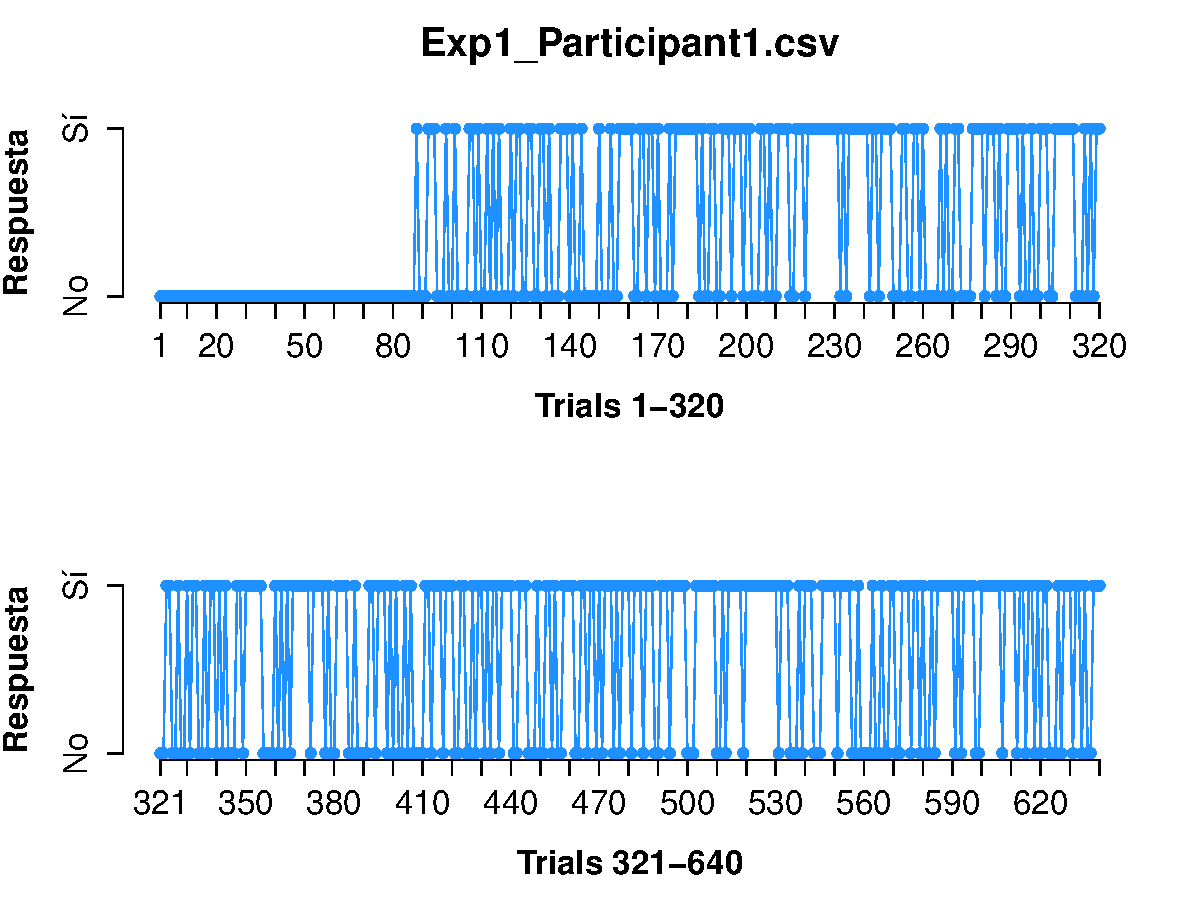
\includegraphics[width=0.30\textwidth]{Figures/Response_Exp1_P1} 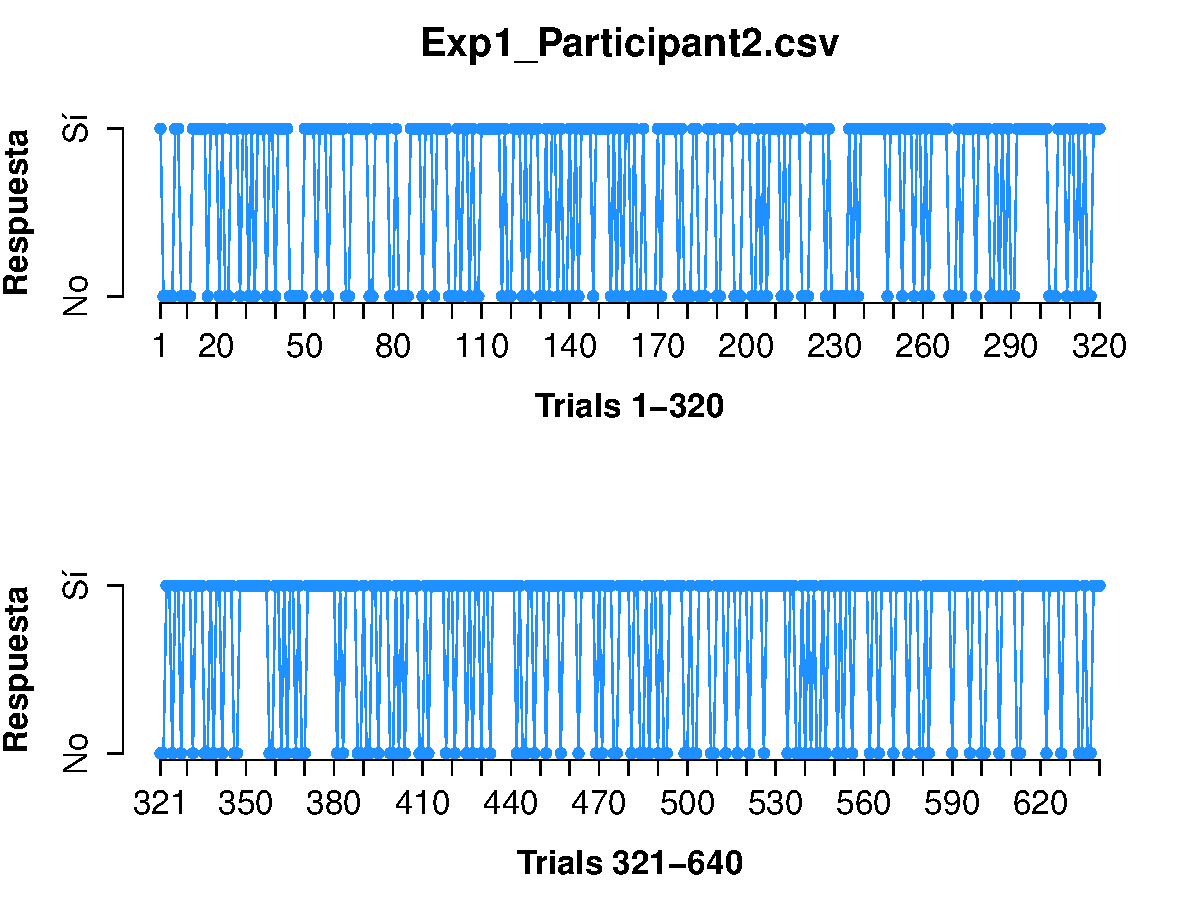
\includegraphics[width=0.30\textwidth]{Figures/Response_Exp1_P2} 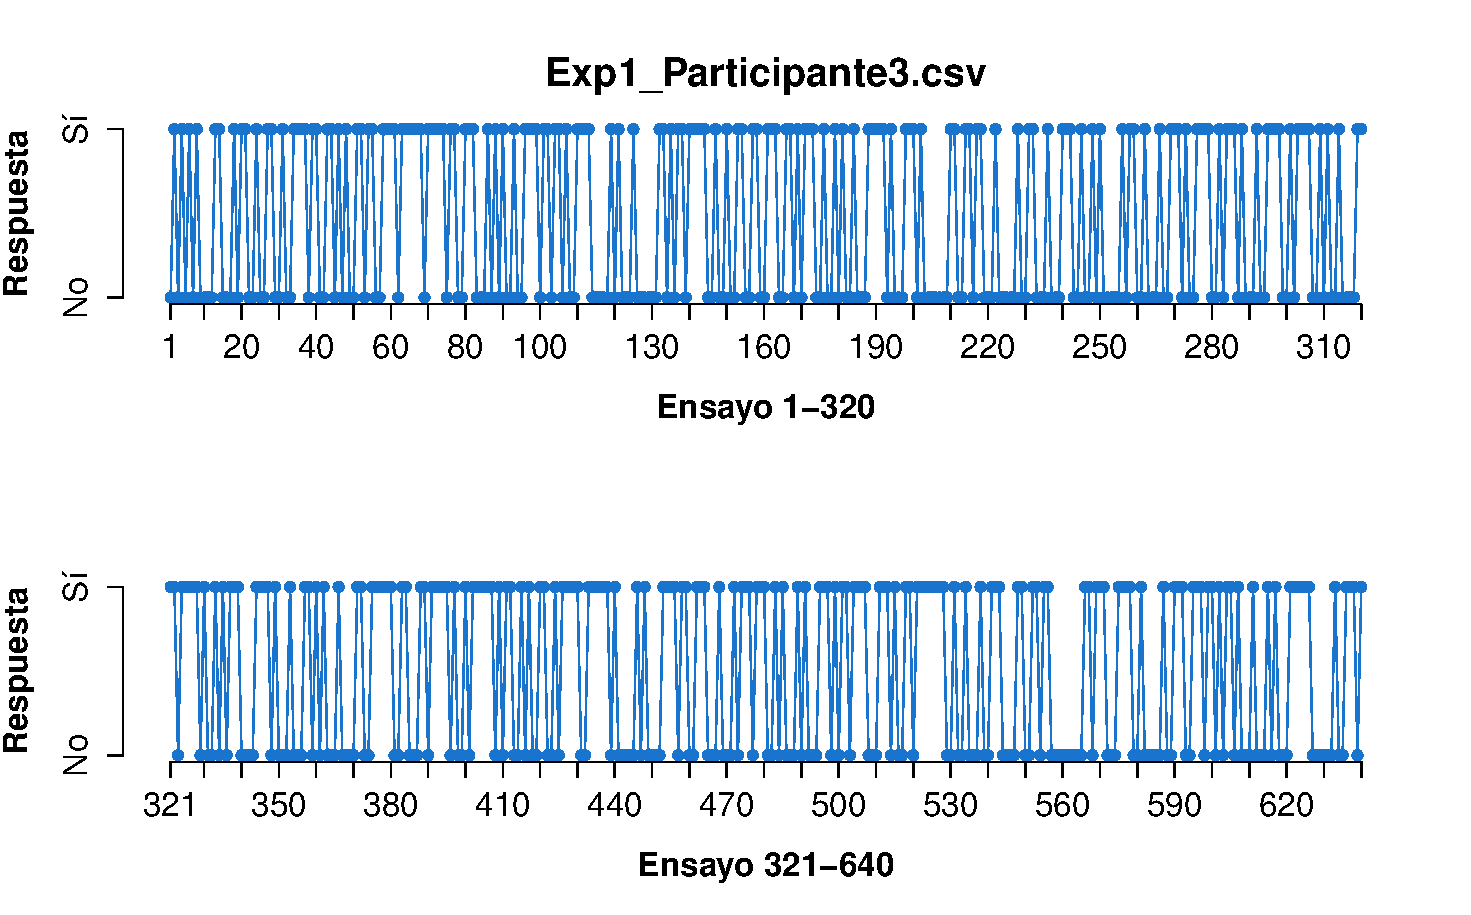
\includegraphics[width=0.30\textwidth]{Figures/Response_Exp1_P3}
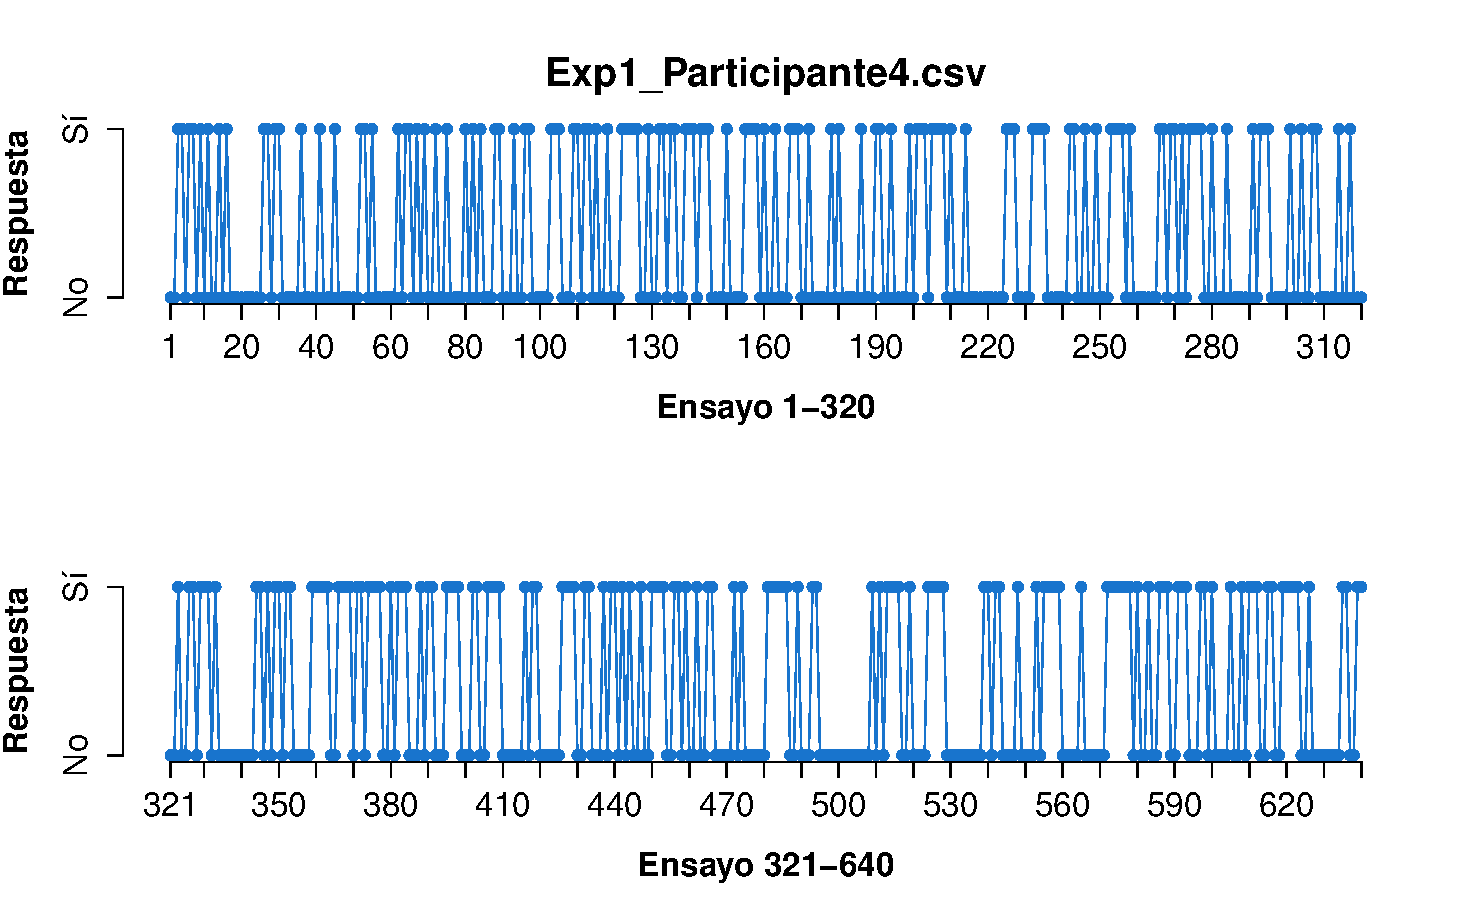
\includegraphics[width=0.30\textwidth]{Figures/Response_Exp1_P4} 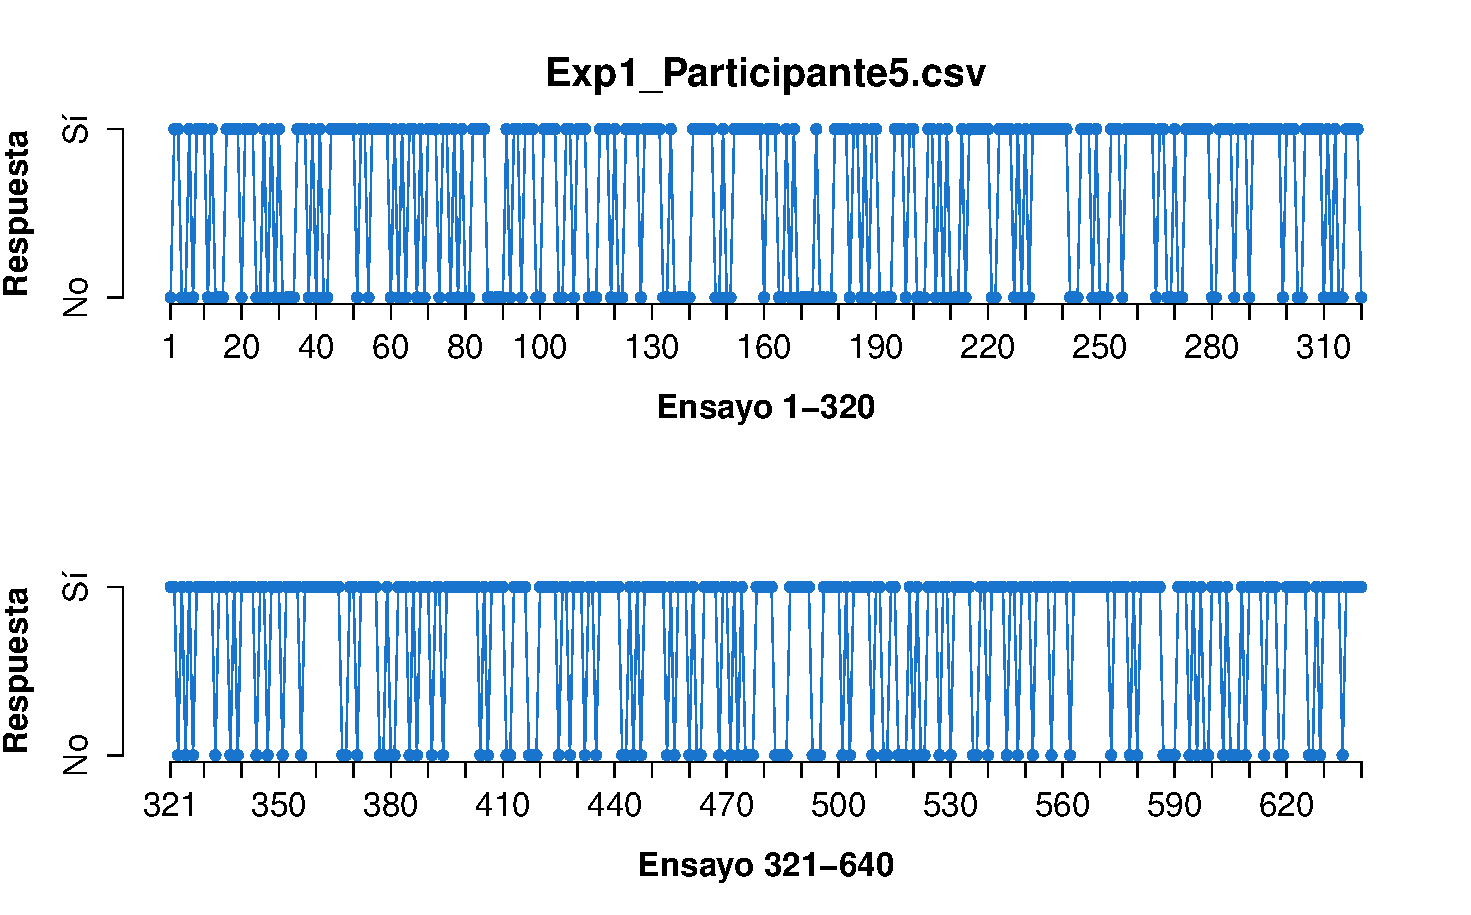
\includegraphics[width=0.30\textwidth]{Figures/Response_Exp1_P5} 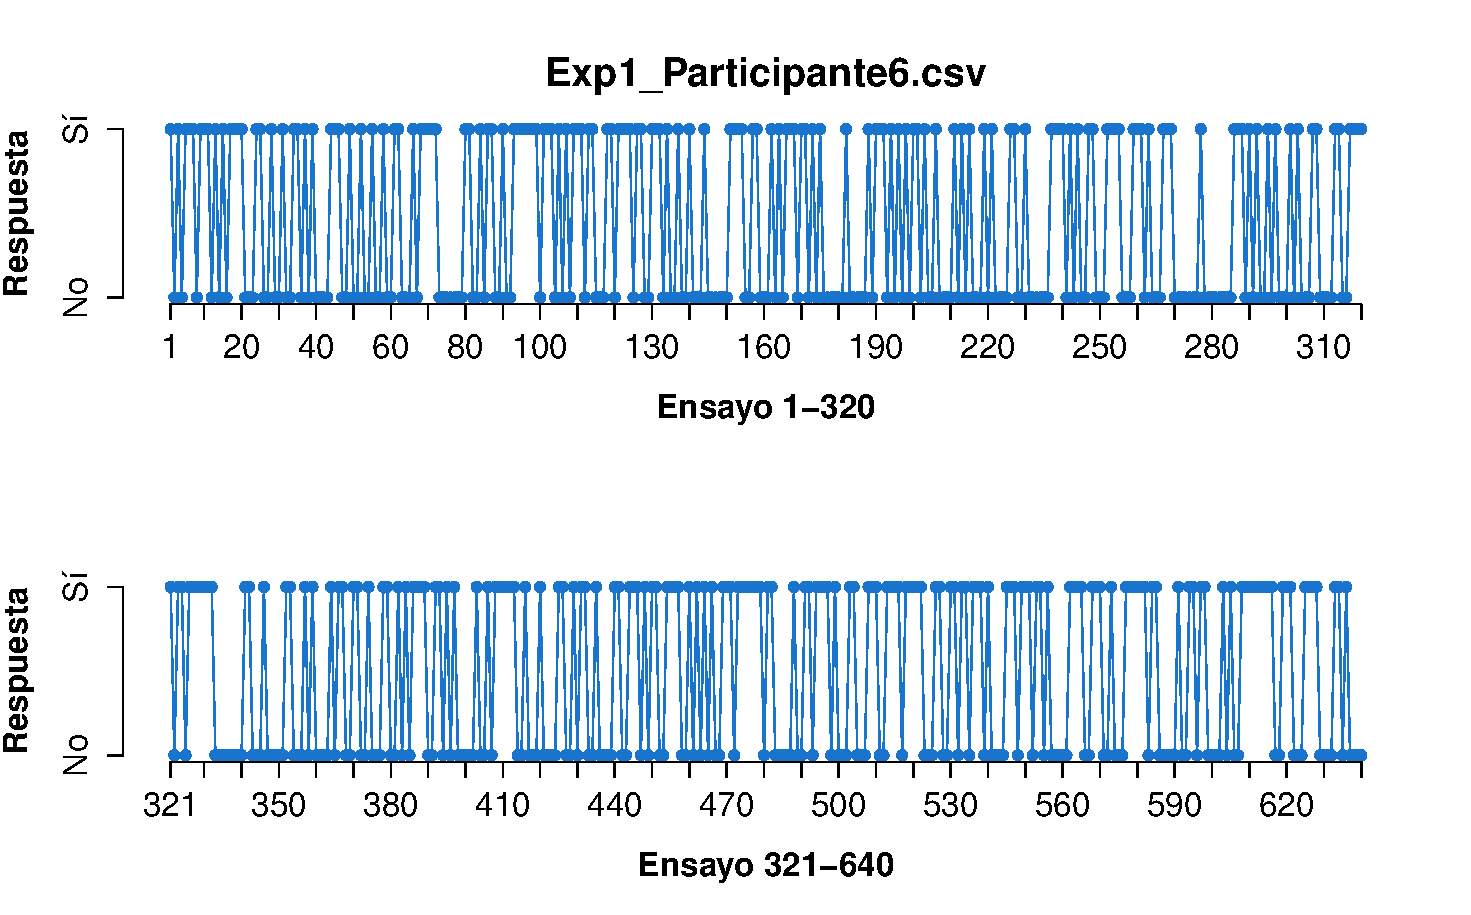
\includegraphics[width=0.30\textwidth]{Figures/Response_Exp1_P6}
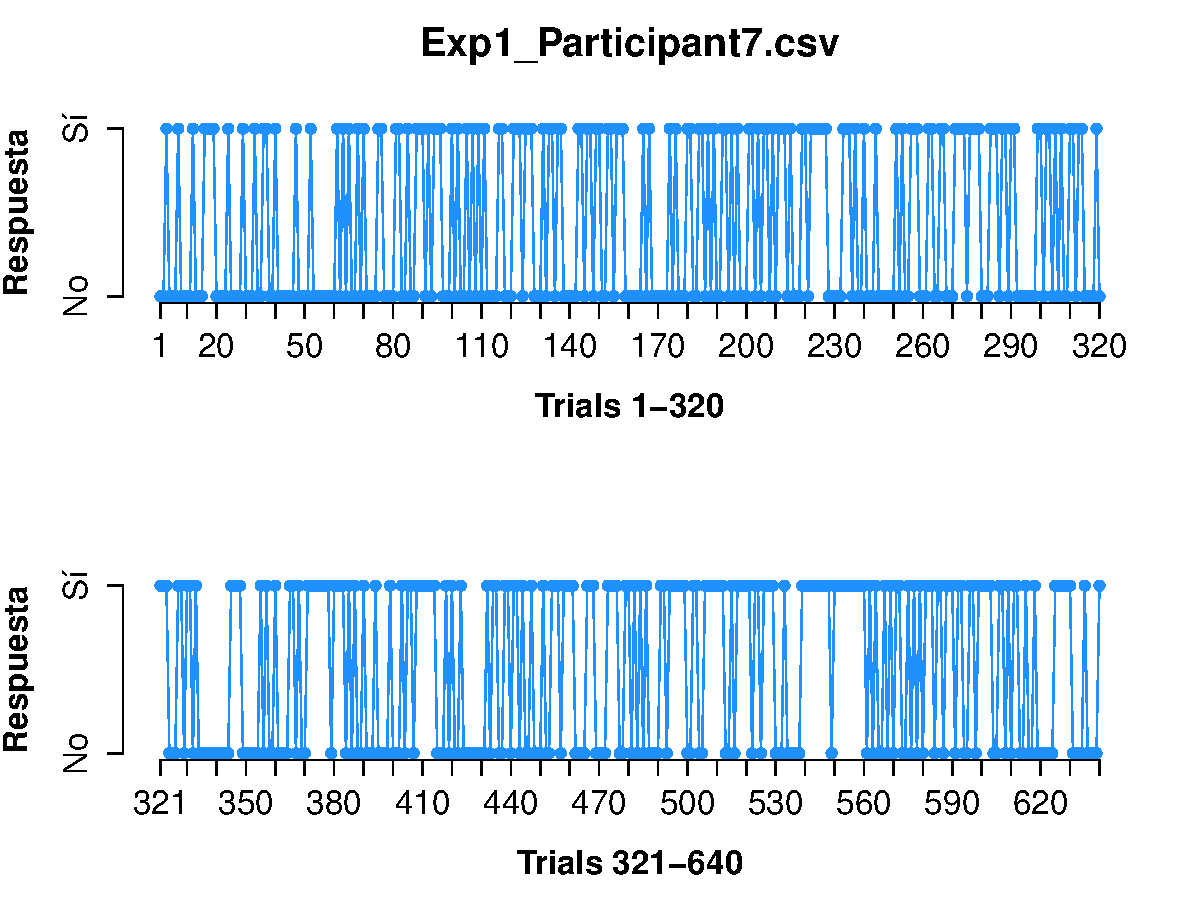
\includegraphics[width=0.30\textwidth]{Figures/Response_Exp1_P7} 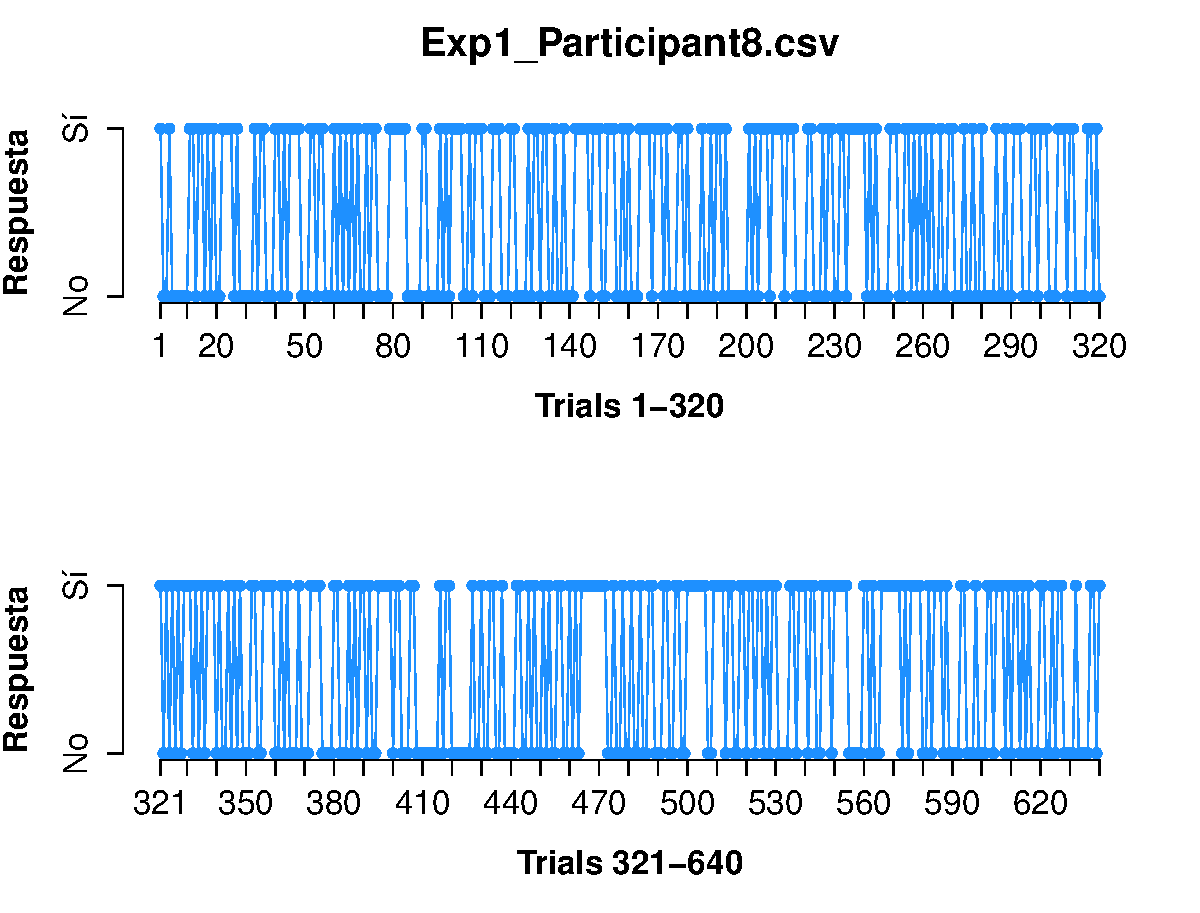
\includegraphics[width=0.30\textwidth]{Figures/Response_Exp1_P8} 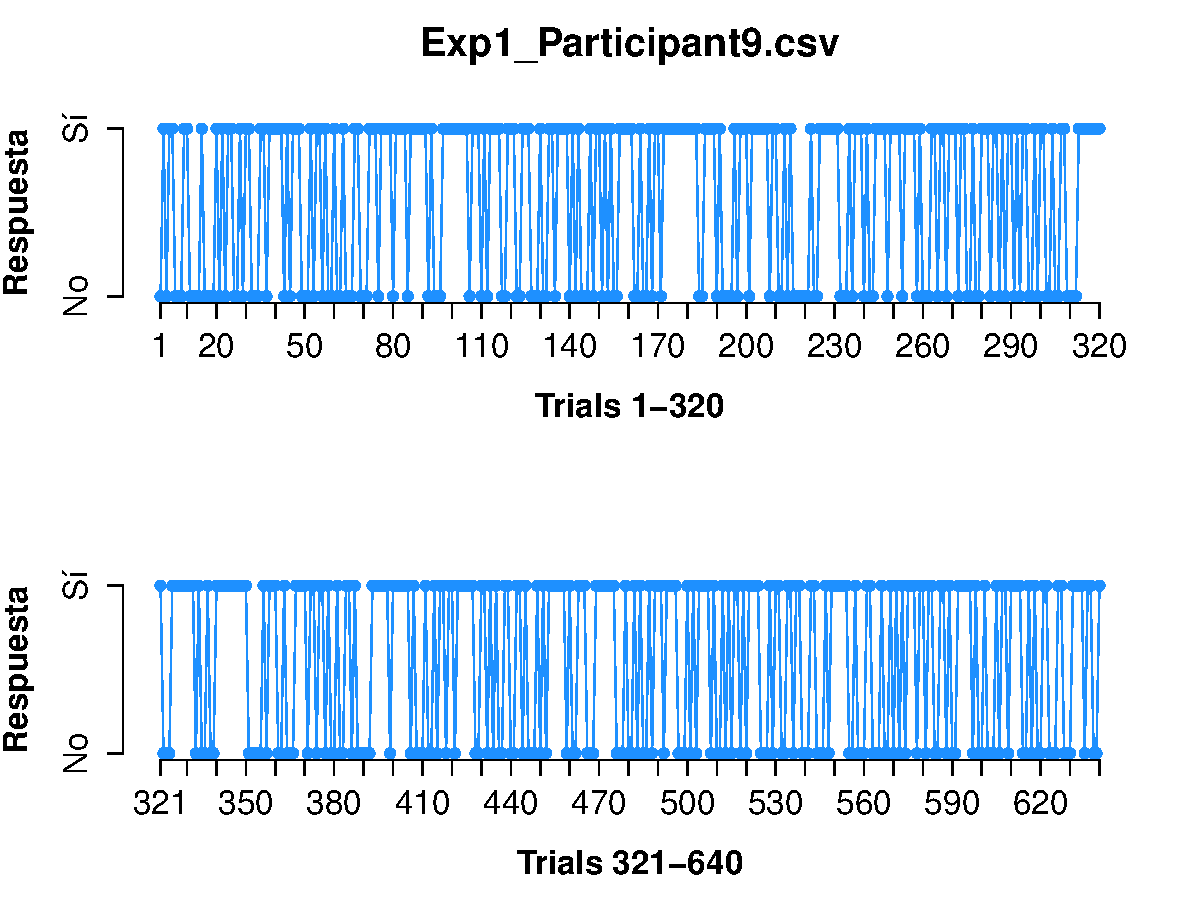
\includegraphics[width=0.30\textwidth]{Figures/Response_Exp1_P9}
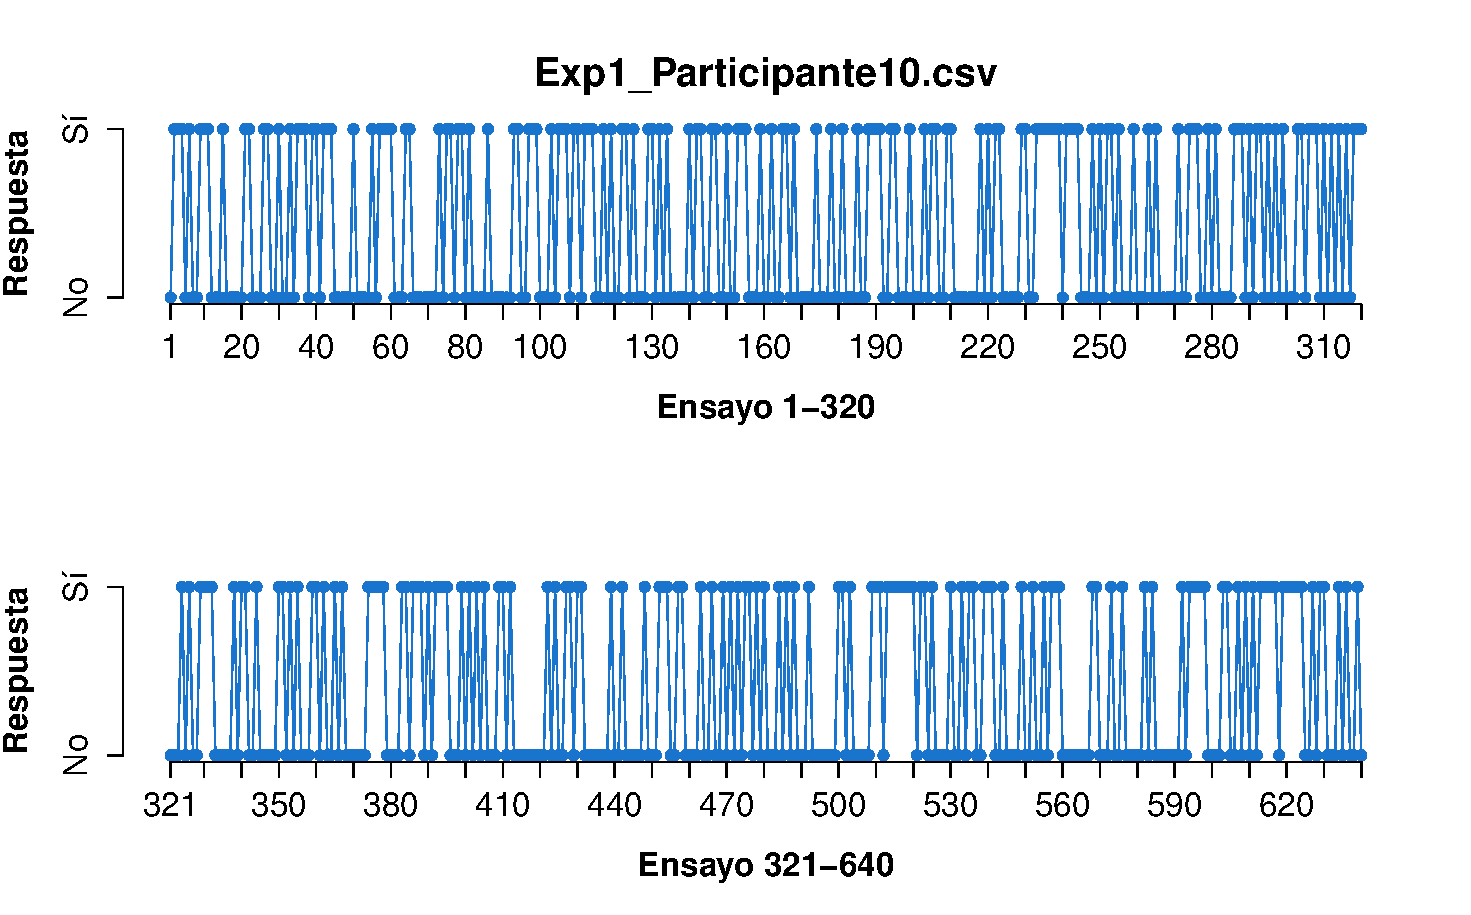
\includegraphics[width=0.30\textwidth]{Figures/Response_Exp1_P10} 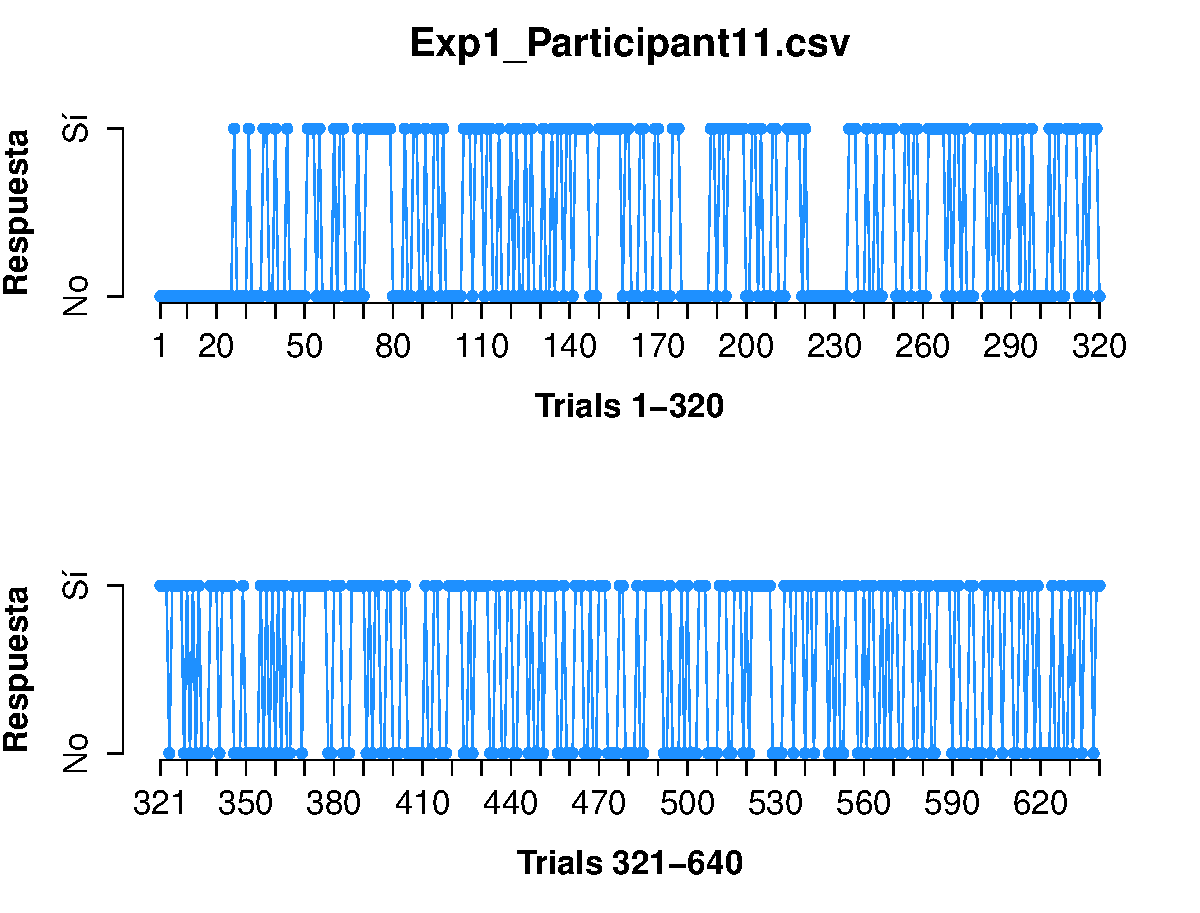
\includegraphics[width=0.30\textwidth]{Figures/Response_Exp1_P11} 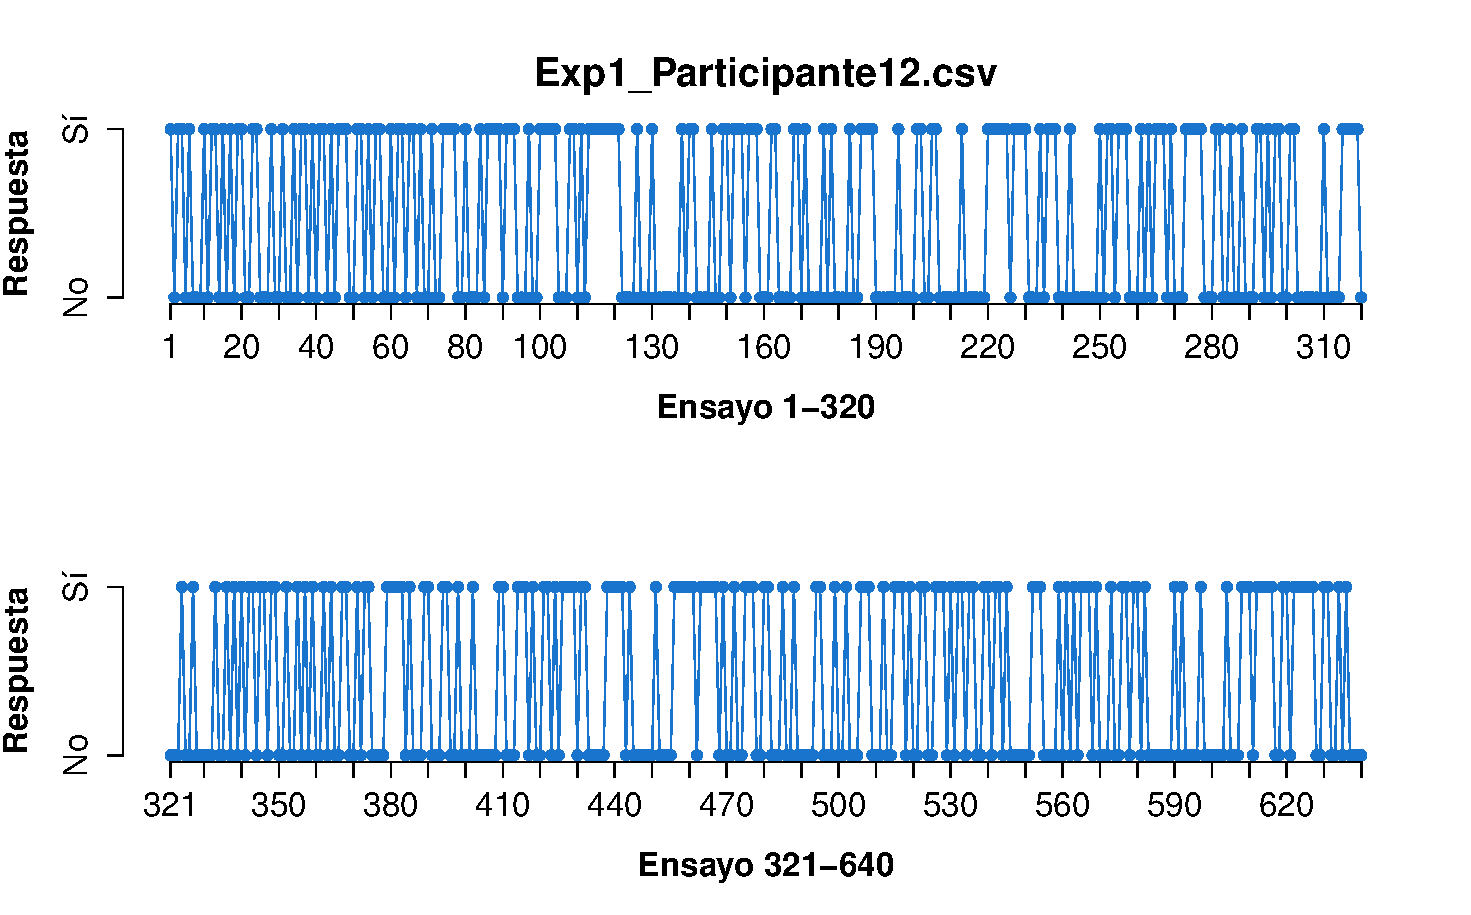
\includegraphics[width=0.30\textwidth]{Figures/Response_Exp1_P12}
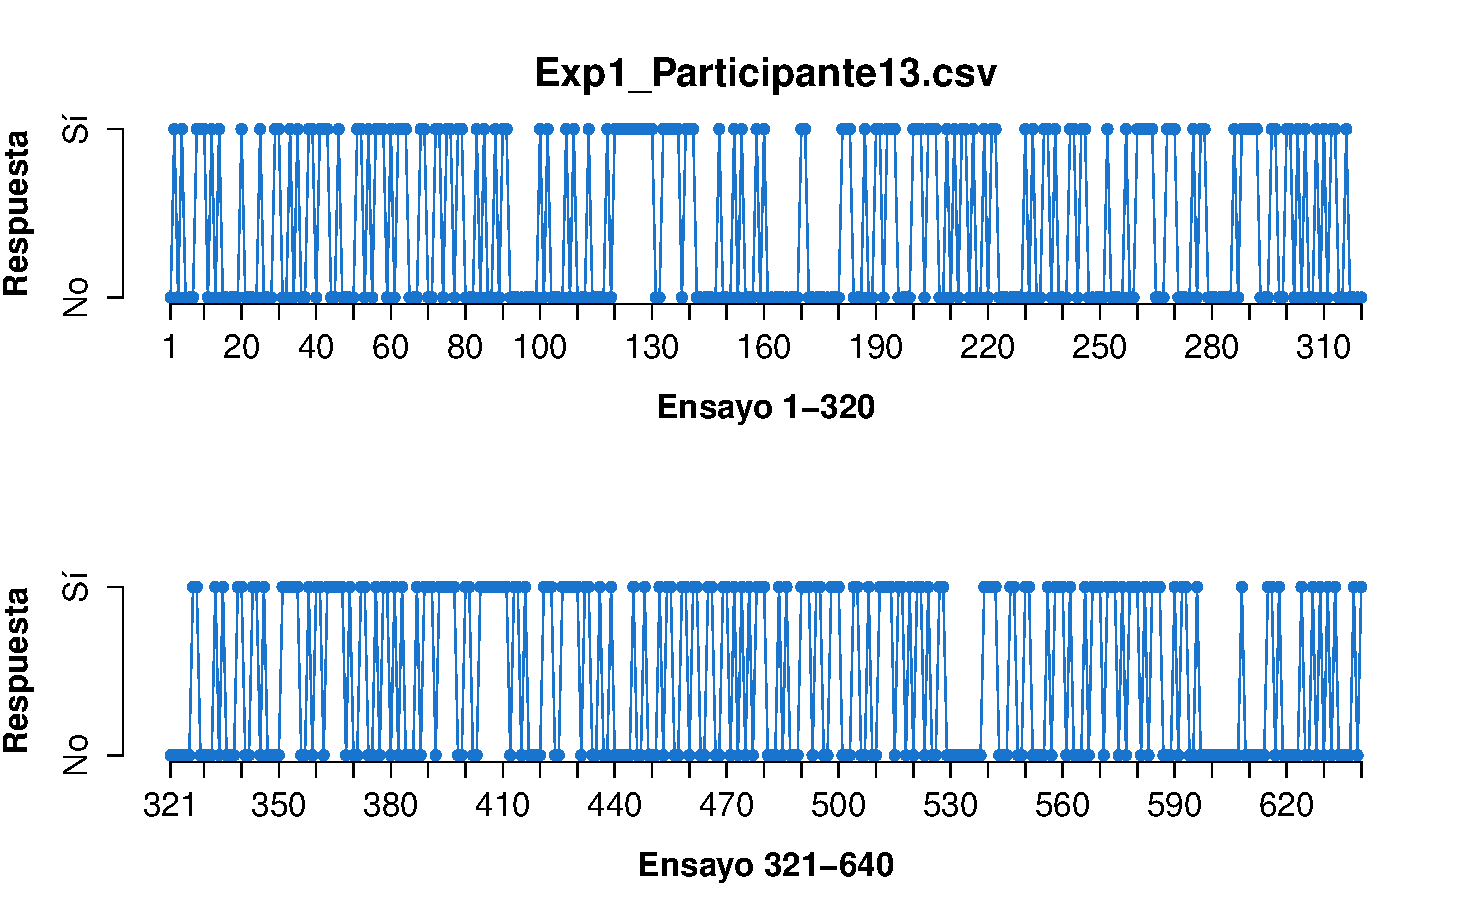
\includegraphics[width=0.30\textwidth]{Figures/Response_Exp1_P13} 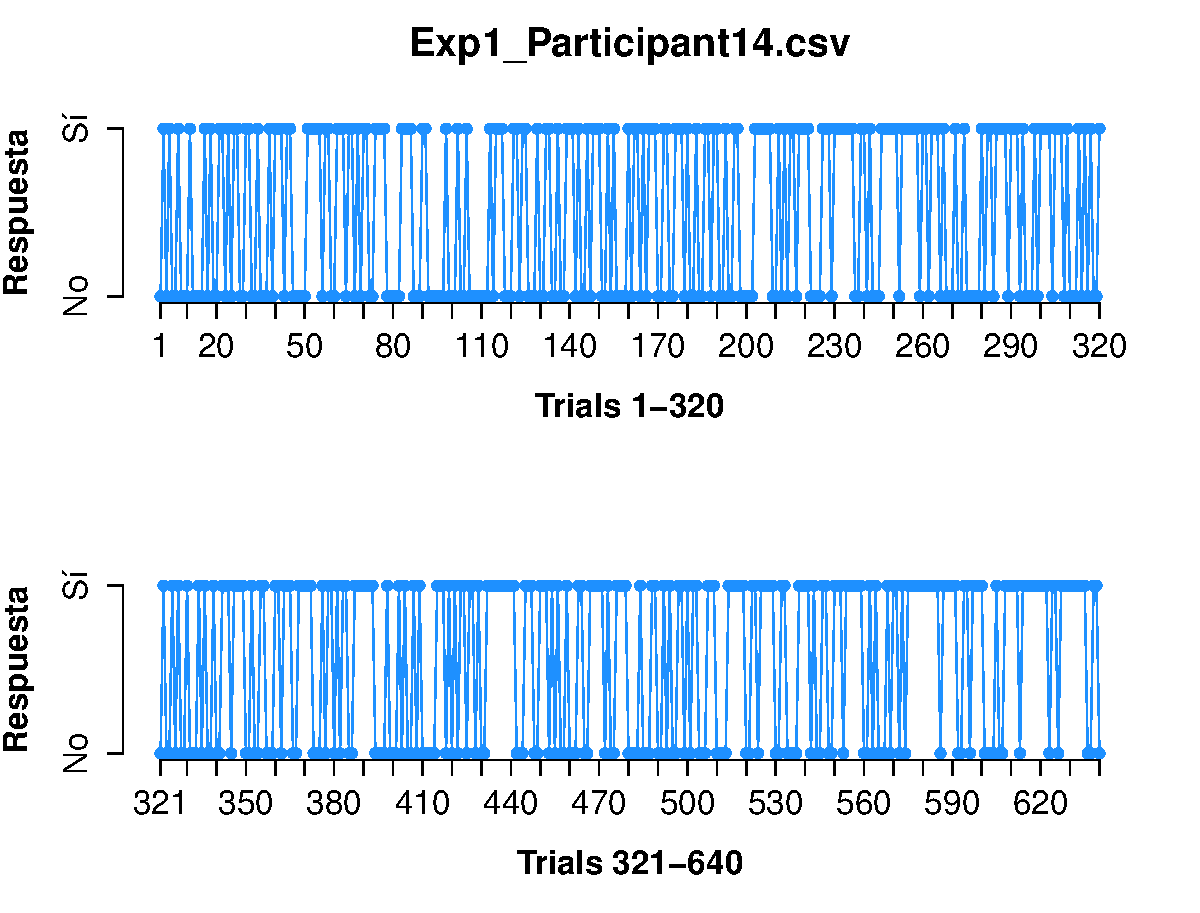
\includegraphics[width=0.30\textwidth]{Figures/Response_Exp1_P14} 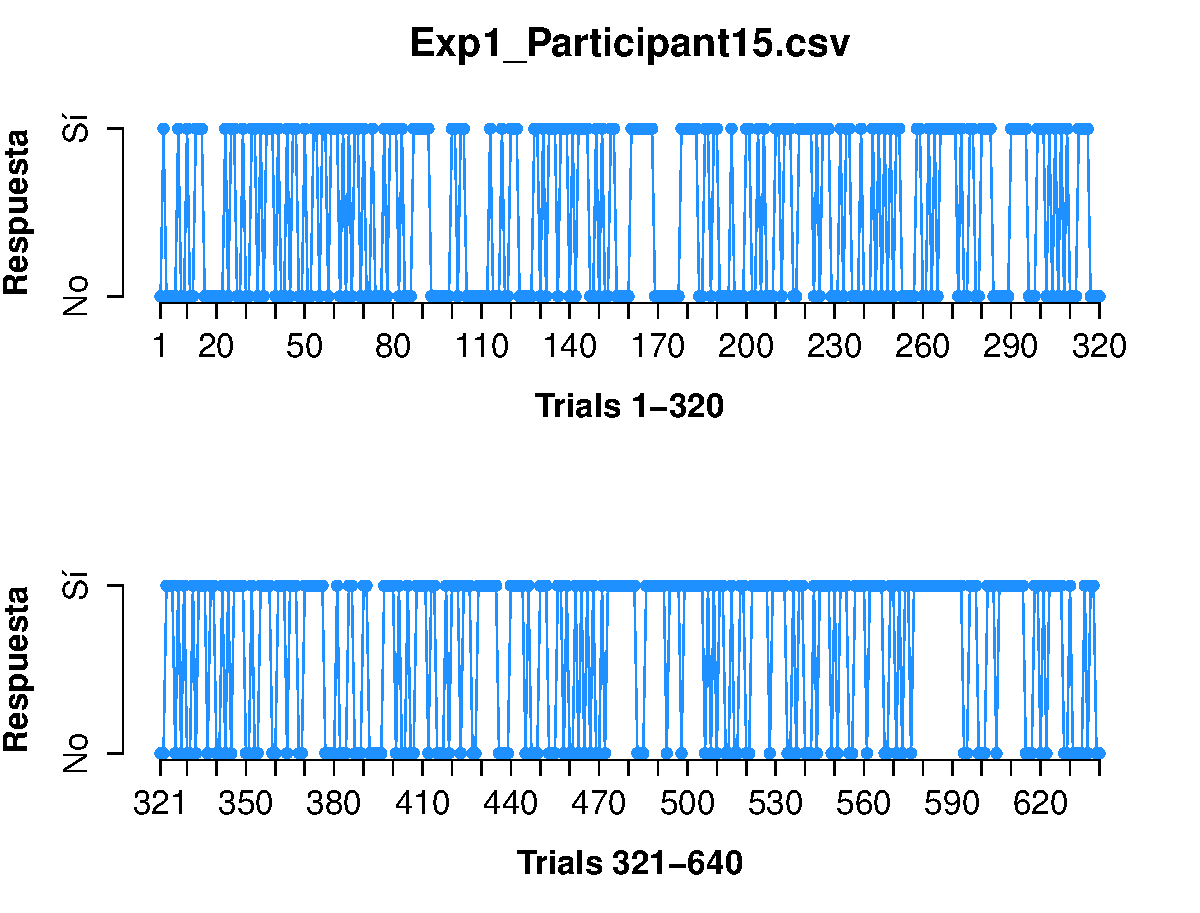
\includegraphics[width=0.30\textwidth]{Figures/Response_Exp1_P15}
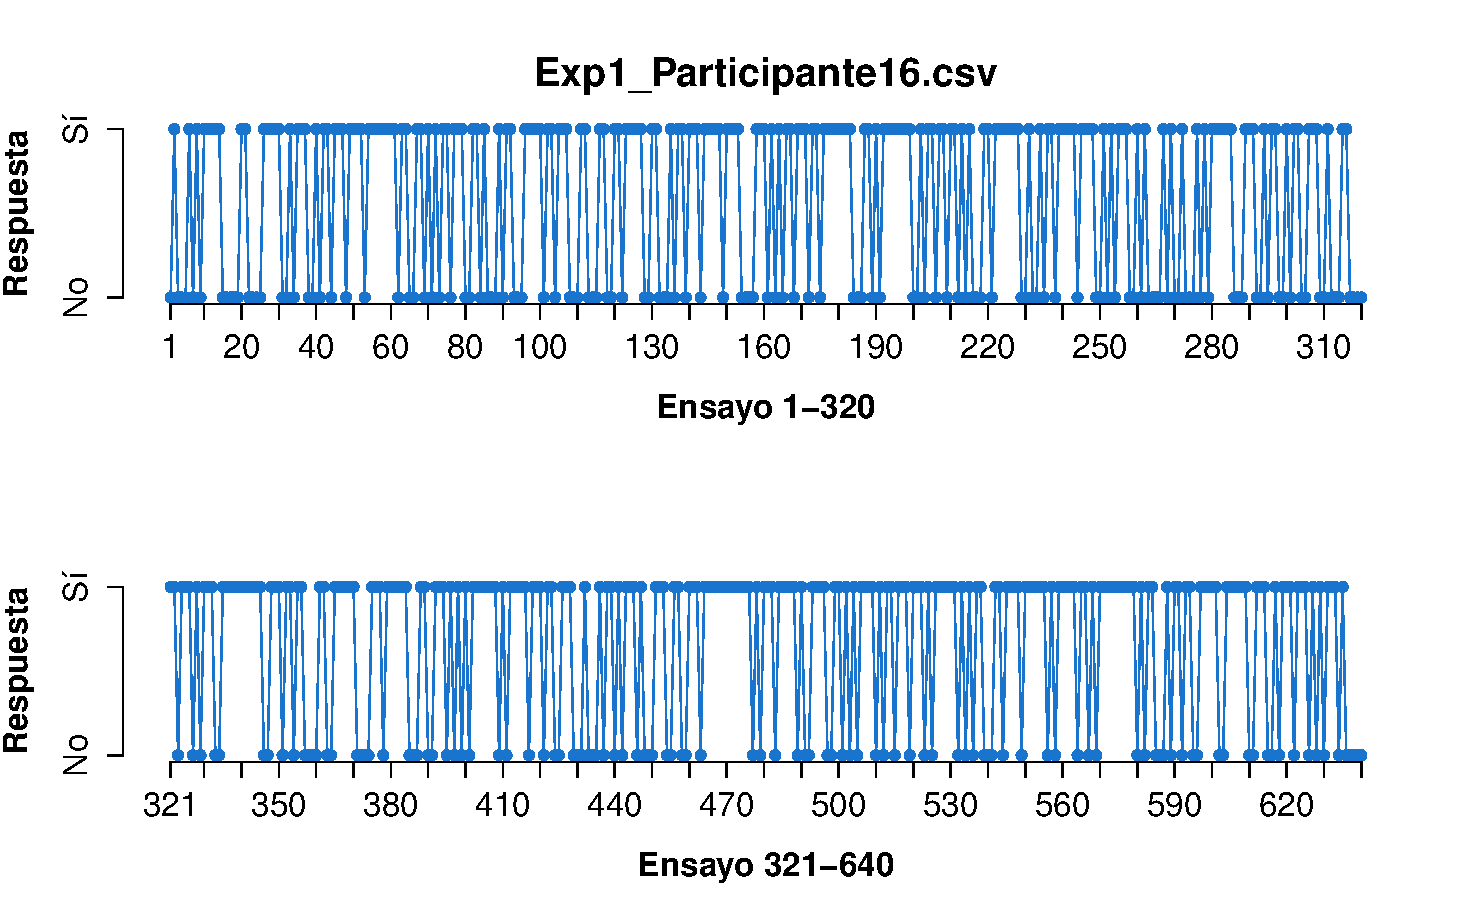
\includegraphics[width=0.30\textwidth]{Figures/Response_Exp1_P16} 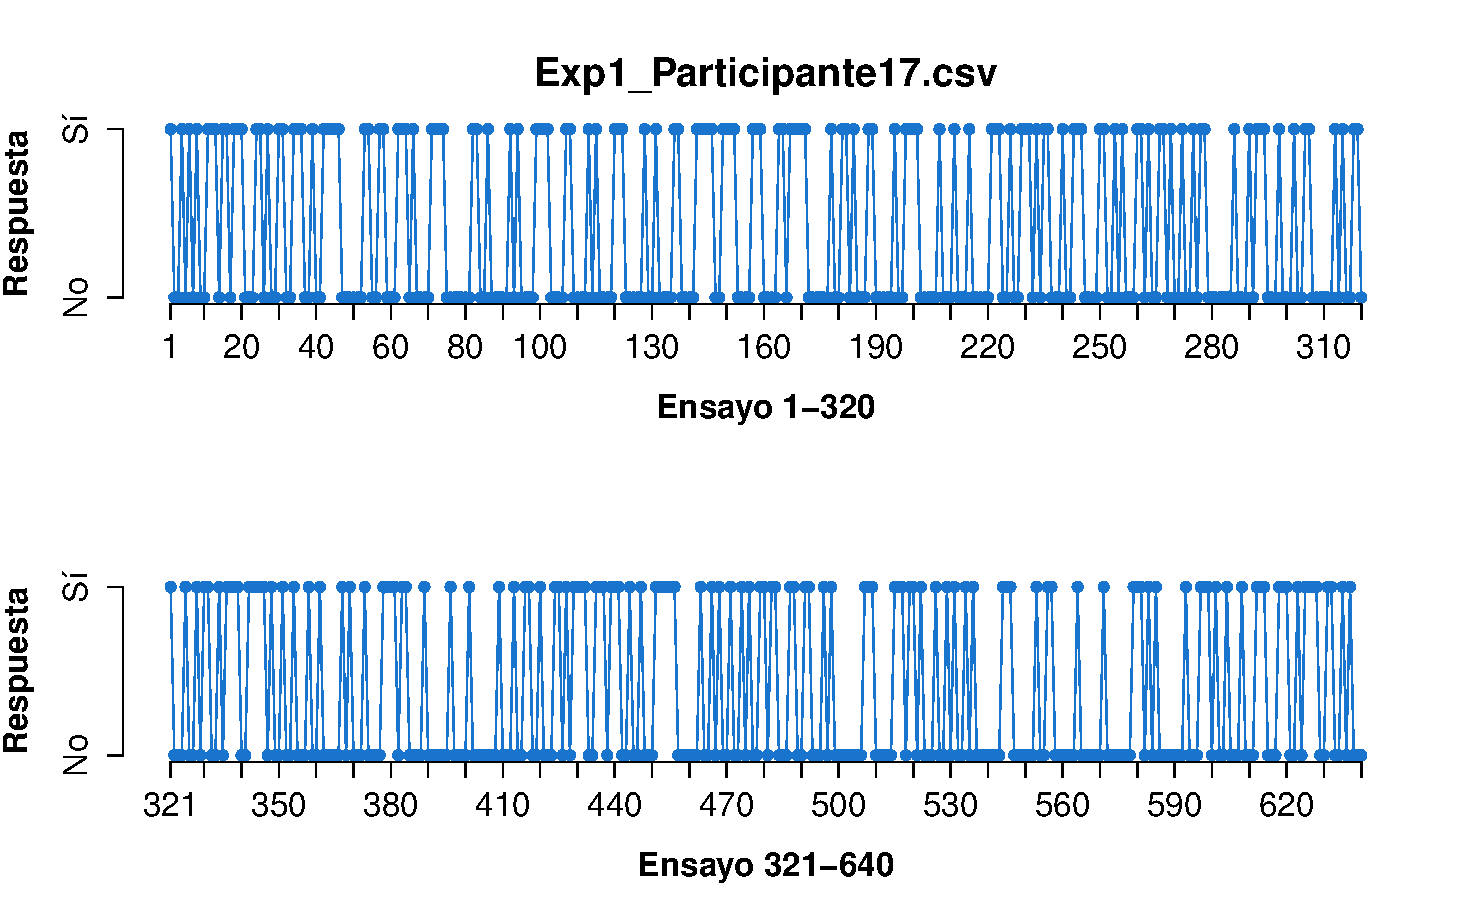
\includegraphics[width=0.30\textwidth]{Figures/Response_Exp1_P17} 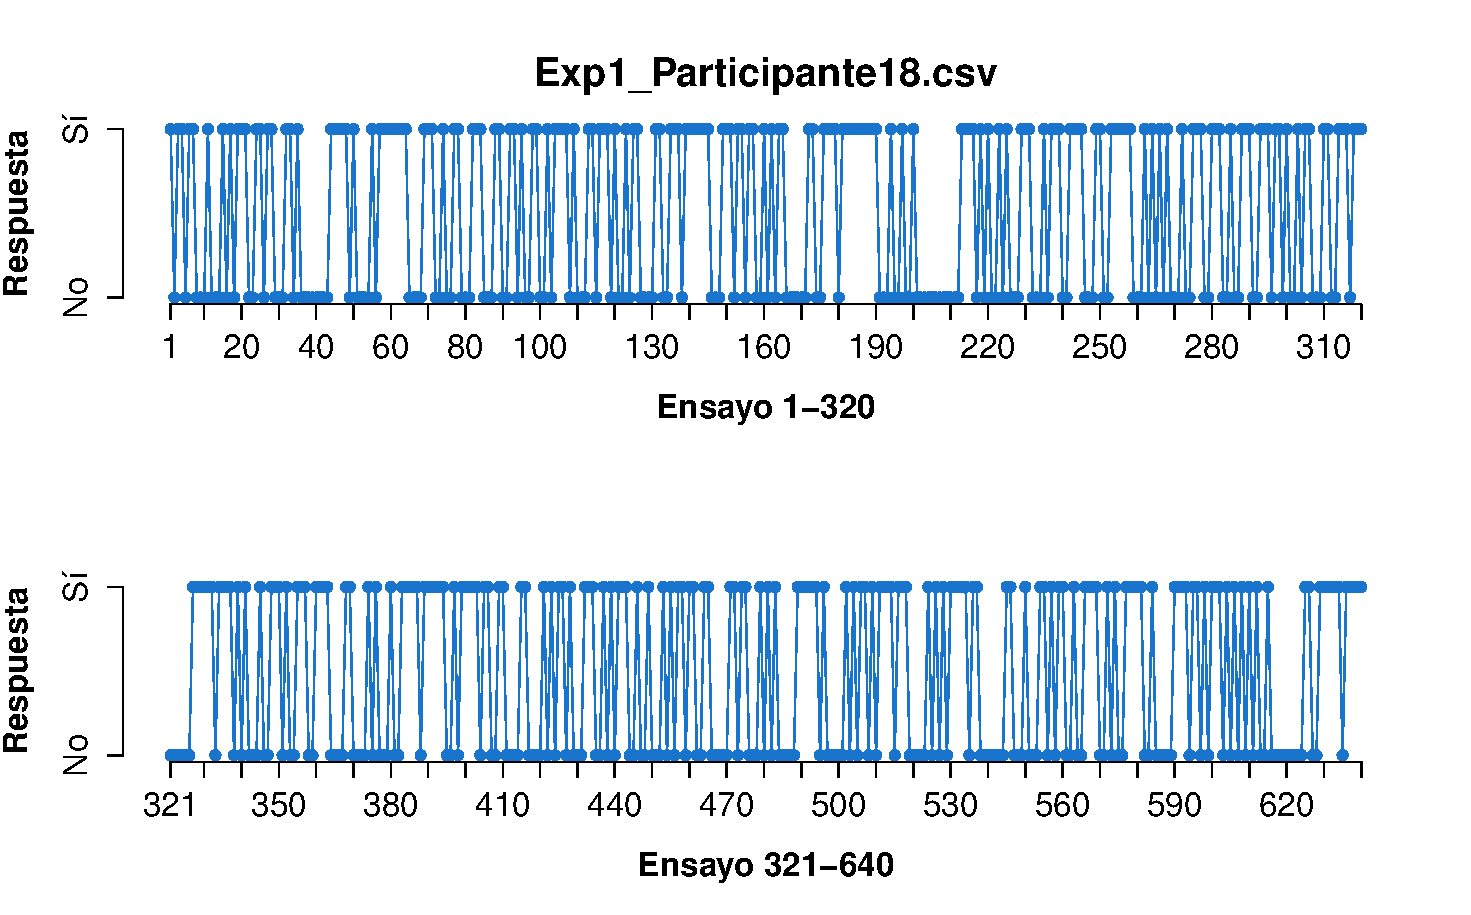
\includegraphics[width=0.30\textwidth]{Figures/Response_Exp1_P18}
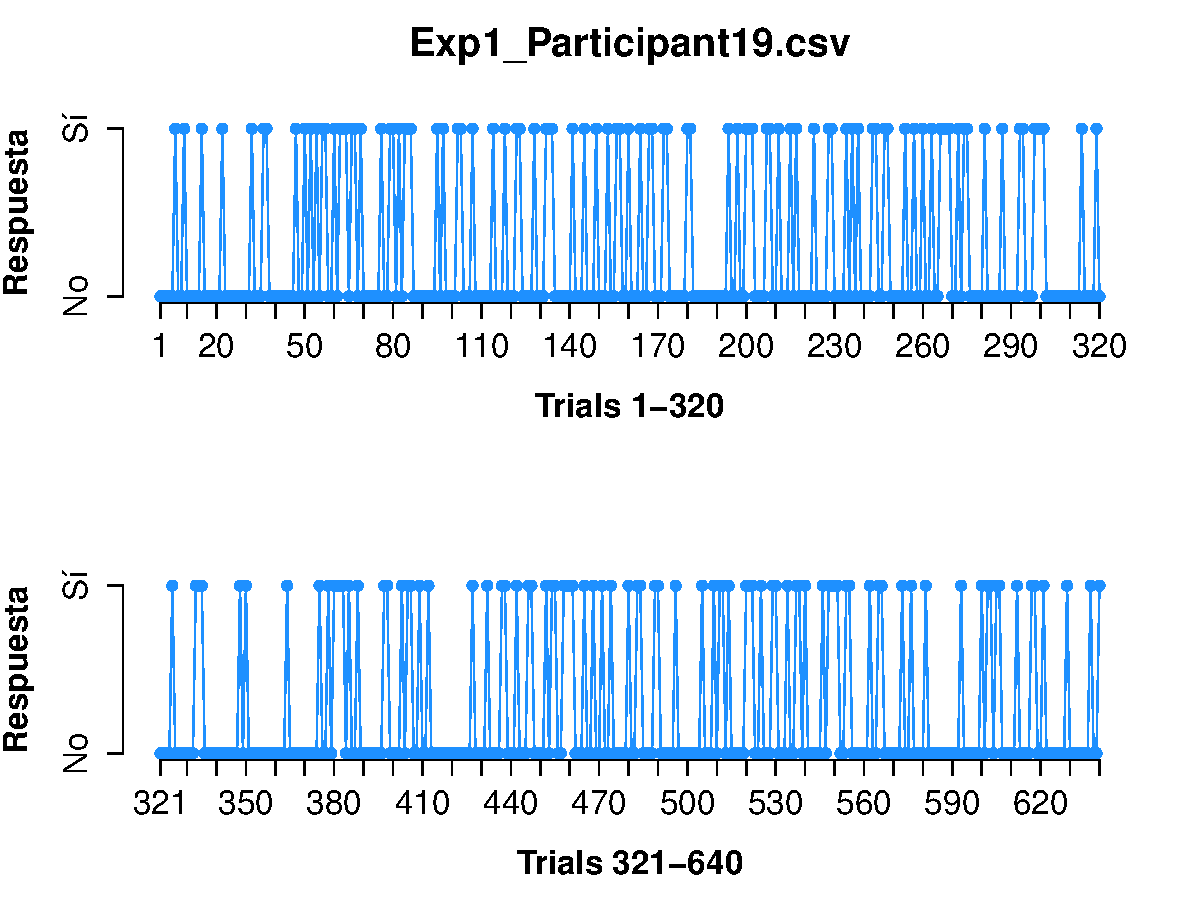
\includegraphics[width=0.30\textwidth]{Figures/Response_Exp1_P19} 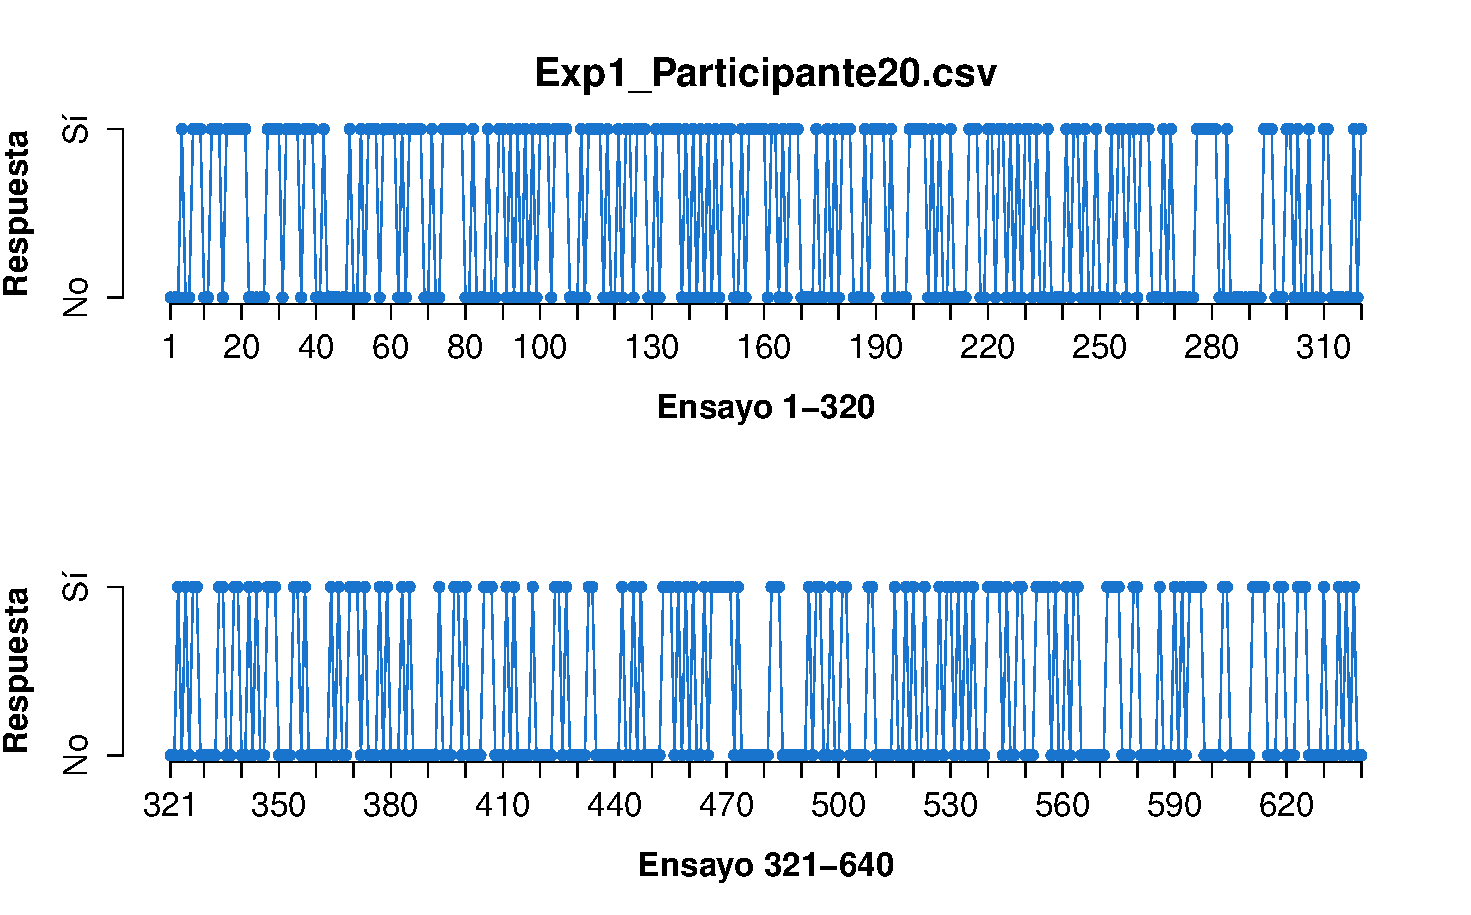
\includegraphics[width=0.30\textwidth]{Figures/Response_Exp1_P20} 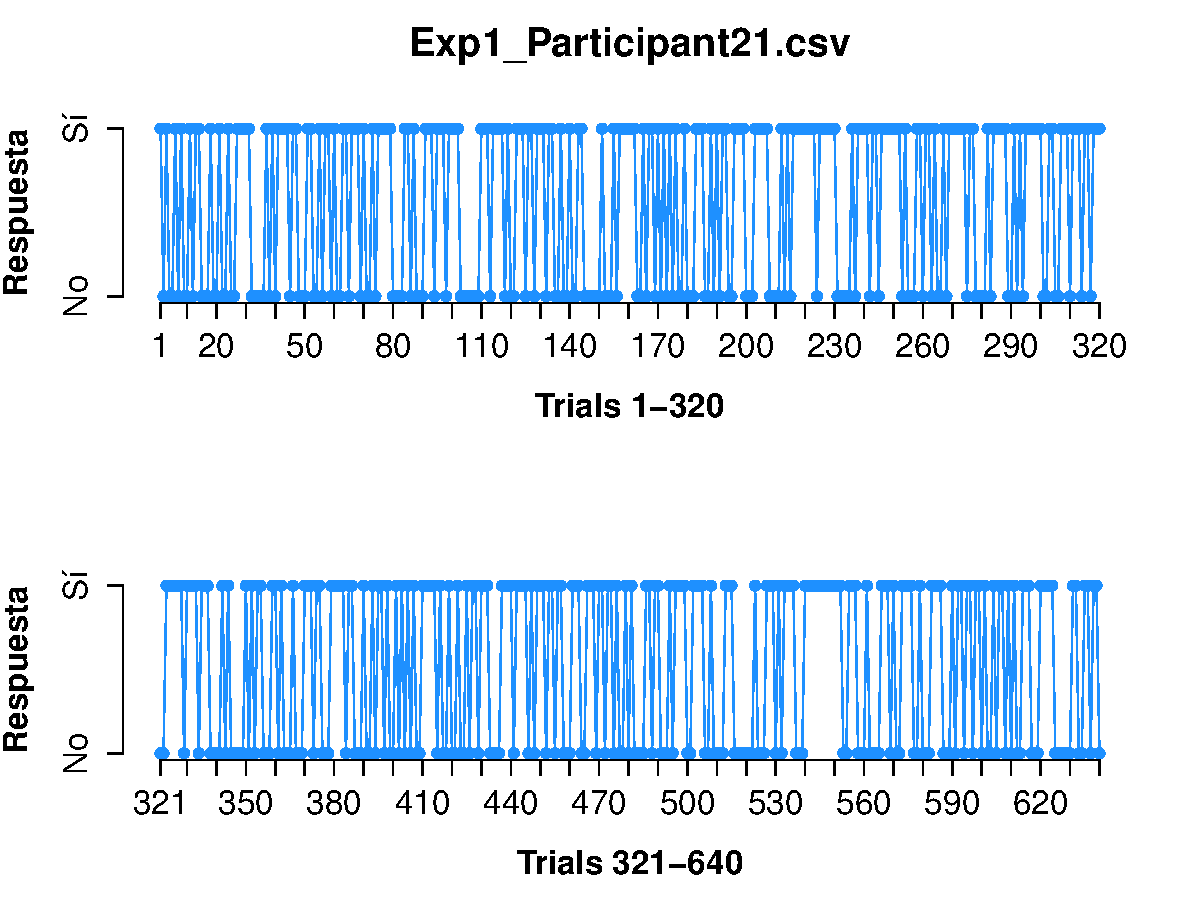
\includegraphics[width=0.30\textwidth]{Figures/Response_Exp1_P21} 
%\decoRule
\caption[Response_Exp1]{Respuesta registrada por cada ensayo (Experimento 1).}
\label{fig:Response_E1}
\end{figure}

\begin{figure}[th]
\centering
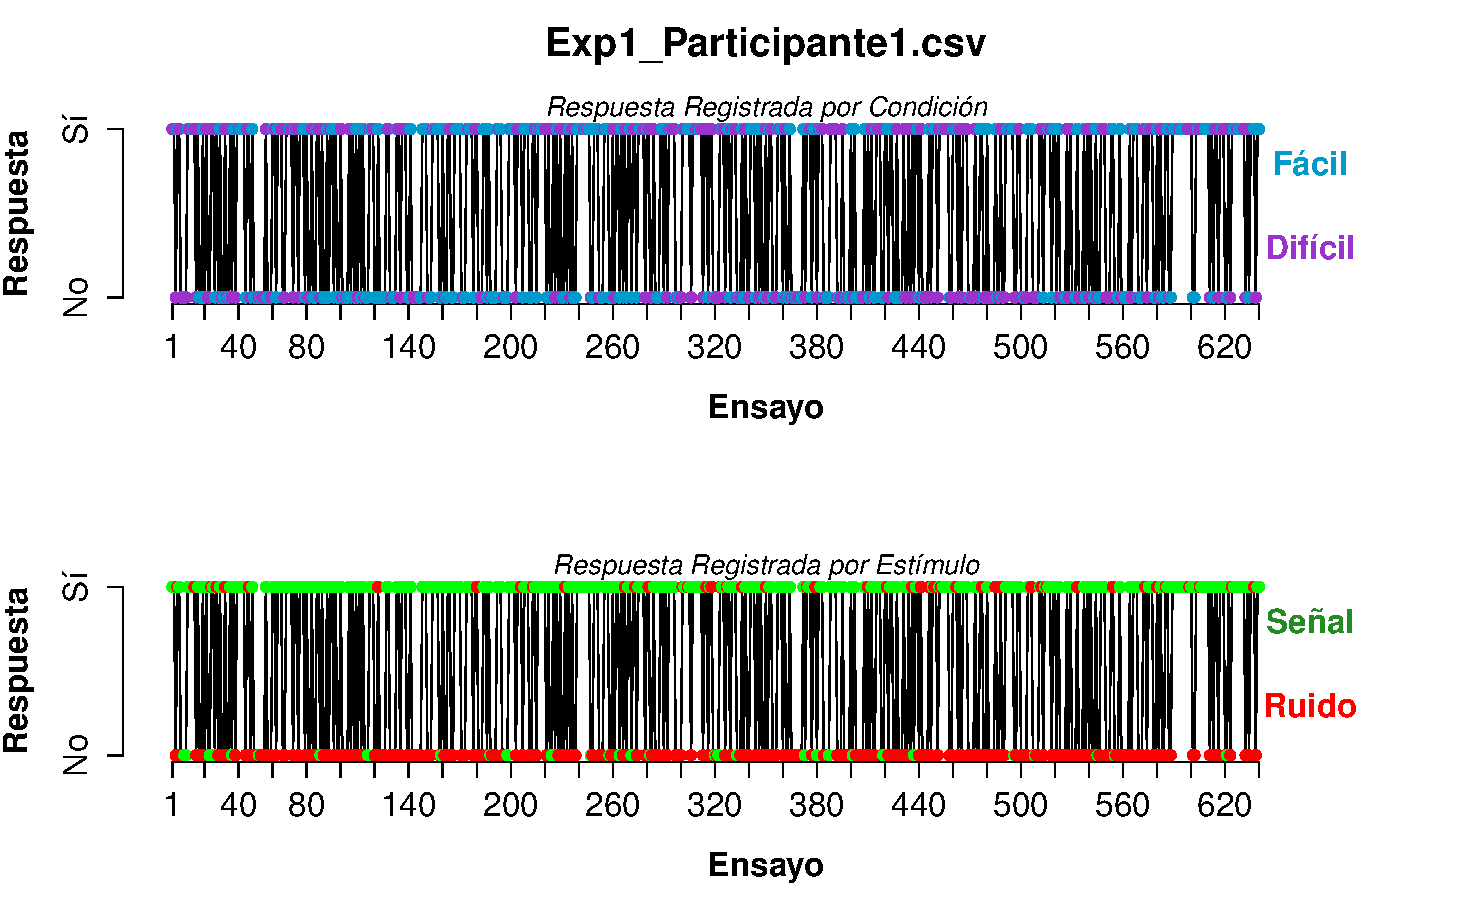
\includegraphics[width=0.30\textwidth]{Figures/BiasResp_Exp1_P1} 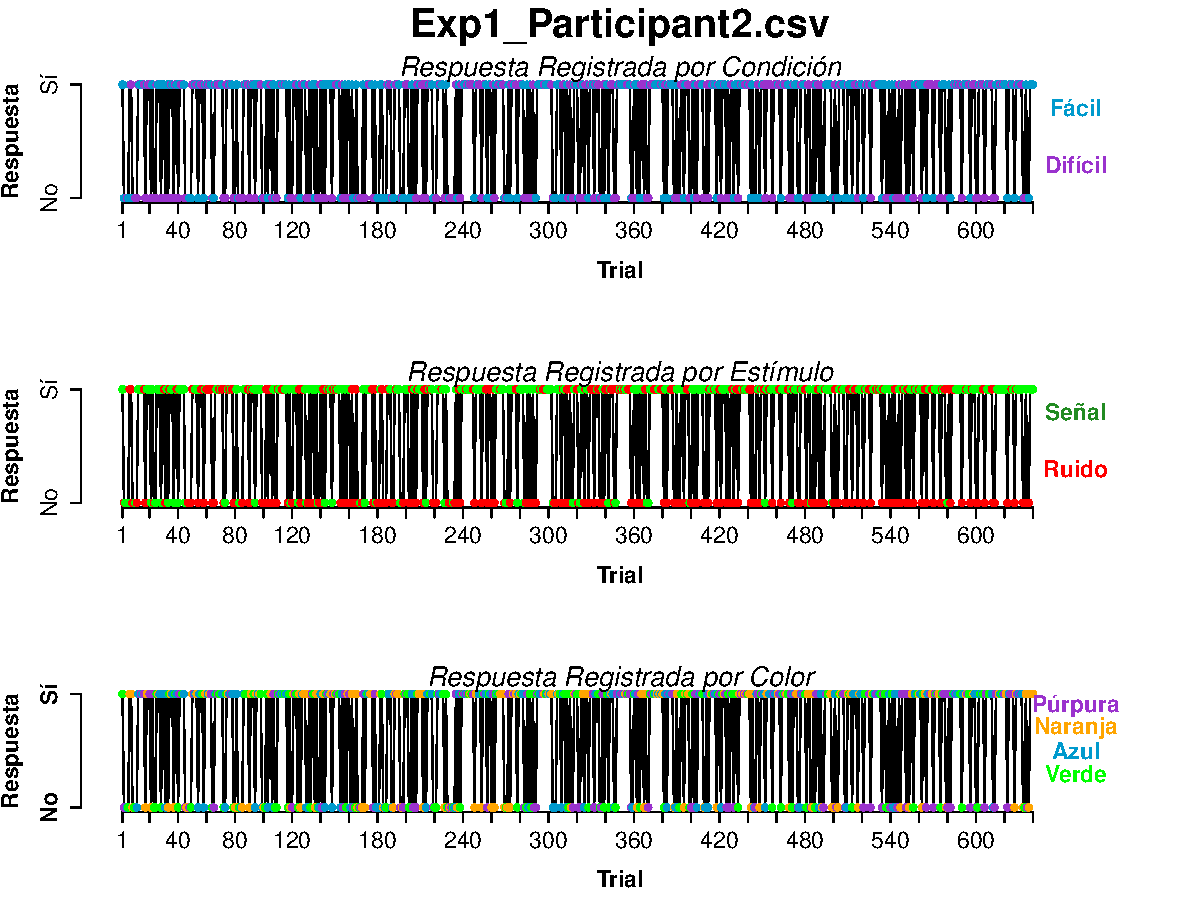
\includegraphics[width=0.30\textwidth]{Figures/BiasResp_Exp1_P2} 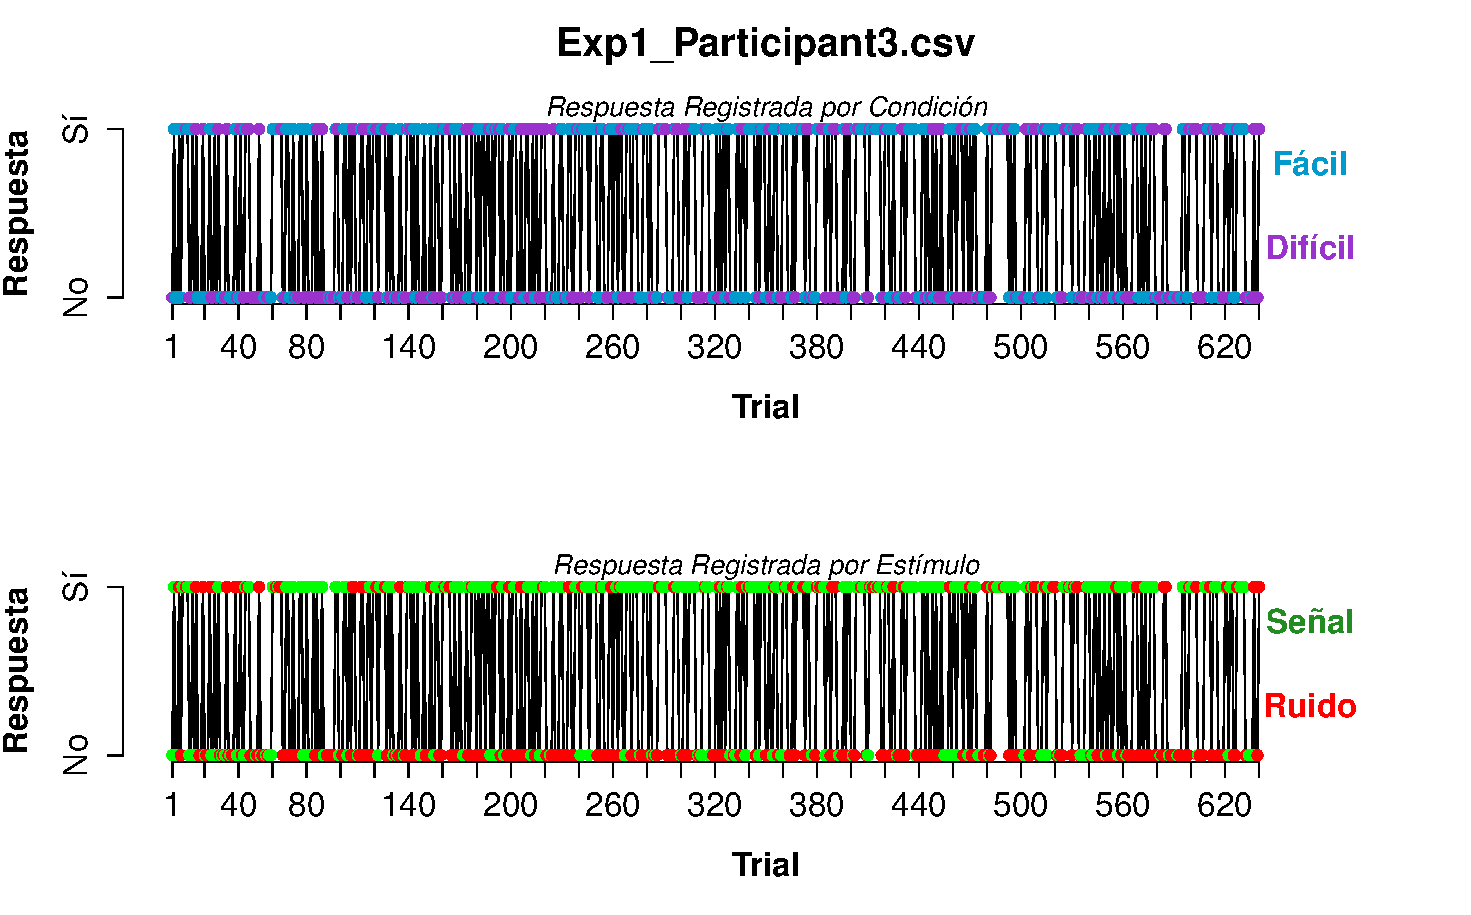
\includegraphics[width=0.30\textwidth]{Figures/BiasResp_Exp1_P3}
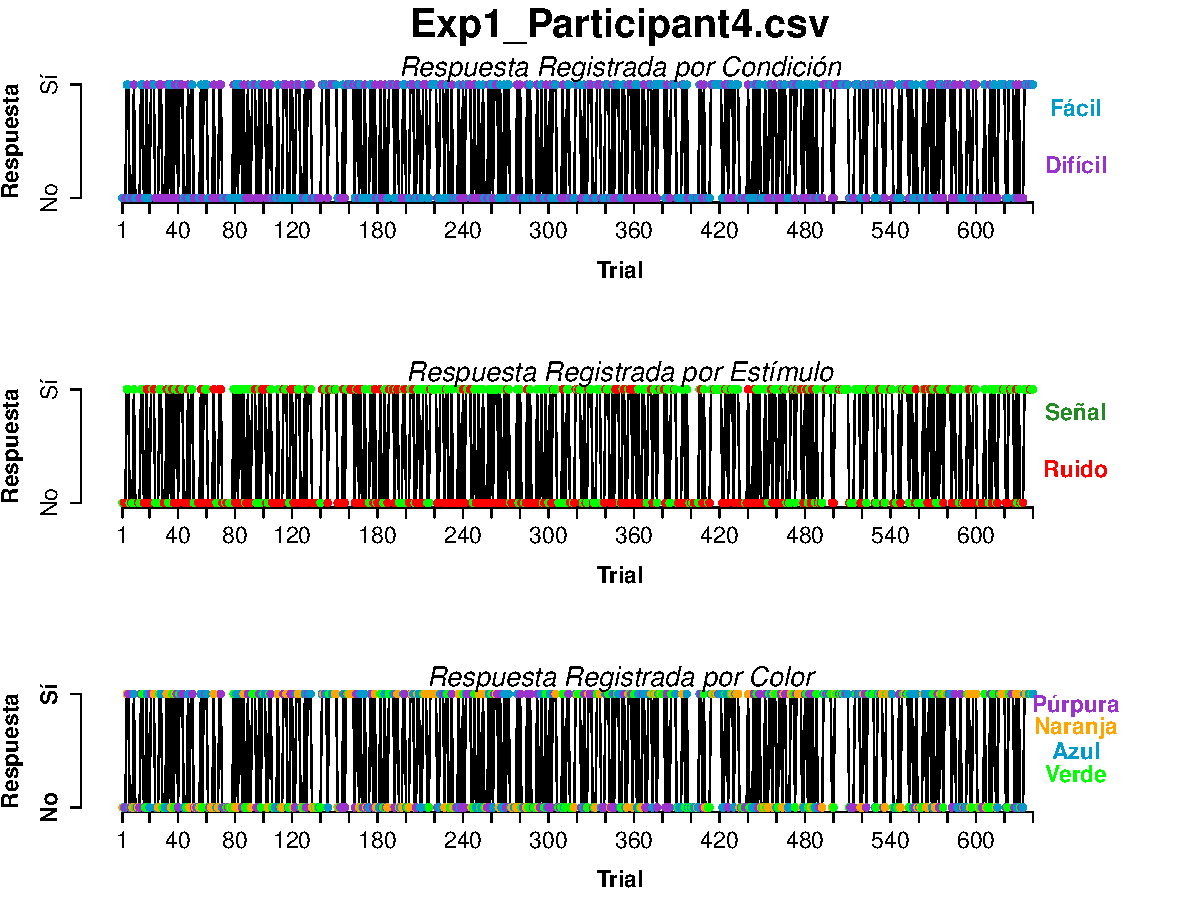
\includegraphics[width=0.30\textwidth]{Figures/BiasResp_Exp1_P4} 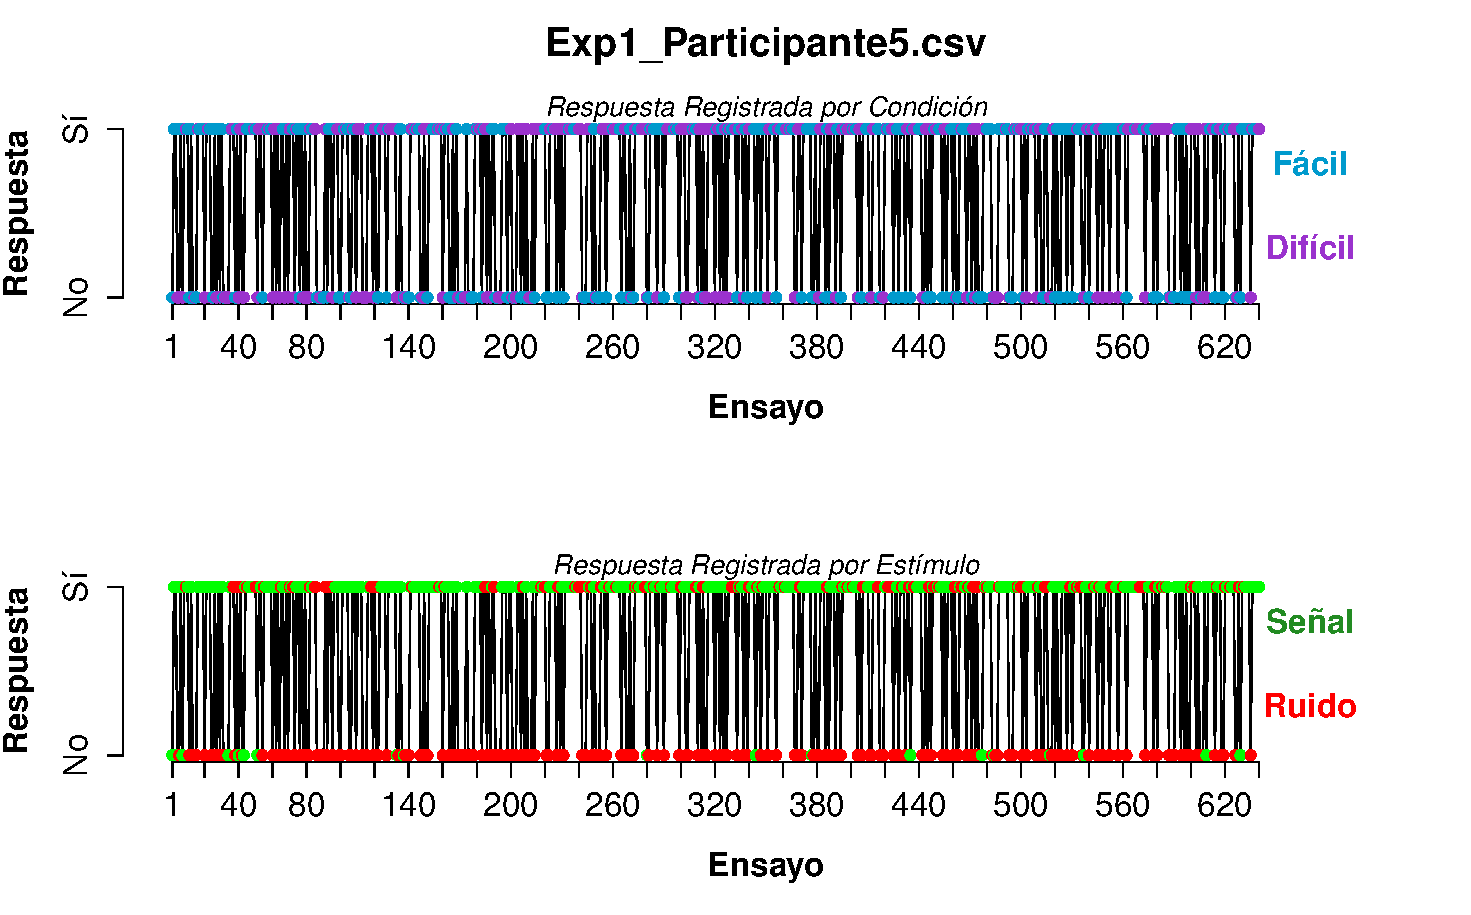
\includegraphics[width=0.30\textwidth]{Figures/BiasResp_Exp1_P5} 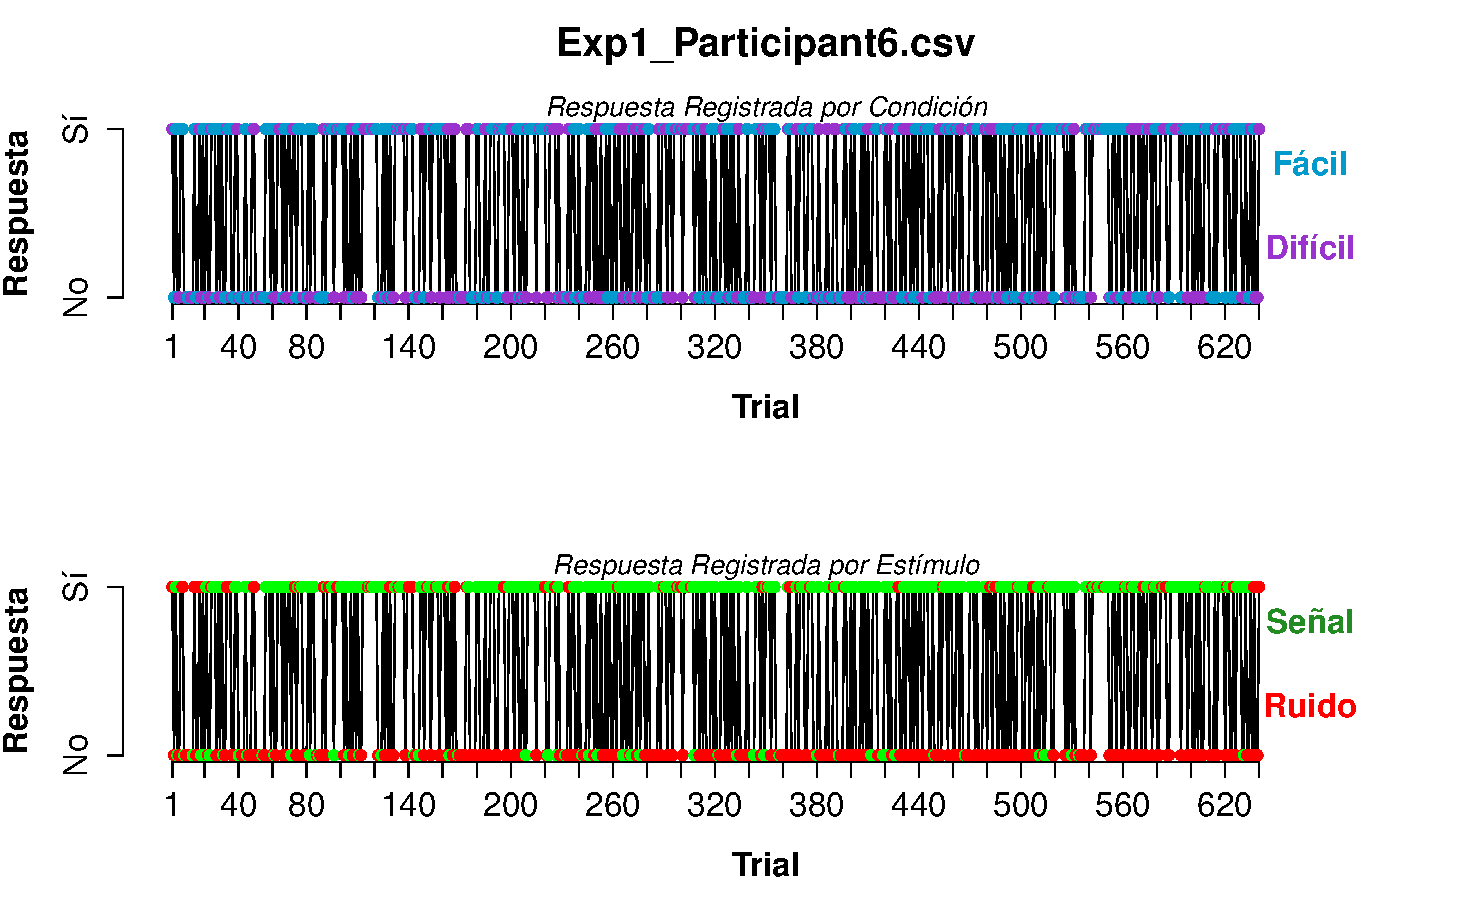
\includegraphics[width=0.30\textwidth]{Figures/BiasResp_Exp1_P6}
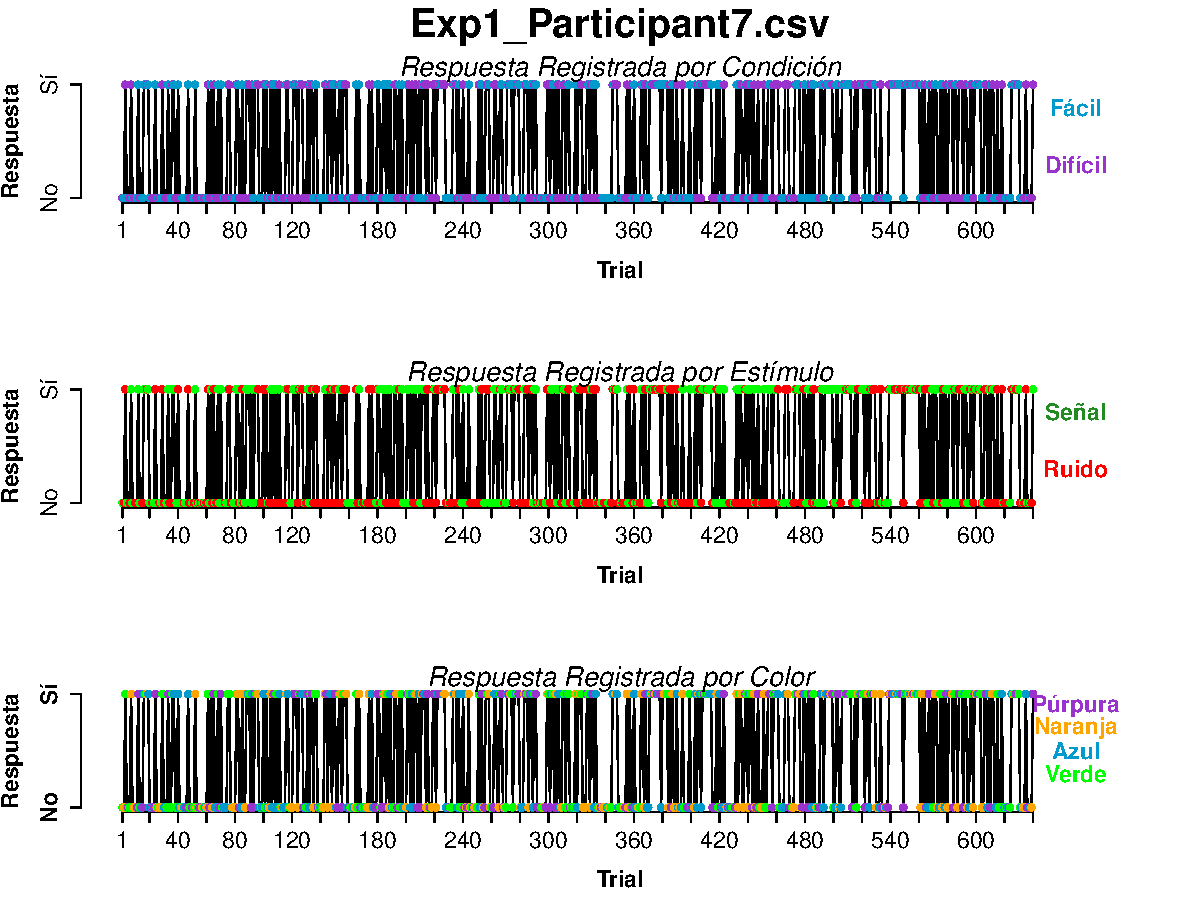
\includegraphics[width=0.30\textwidth]{Figures/BiasResp_Exp1_P7} 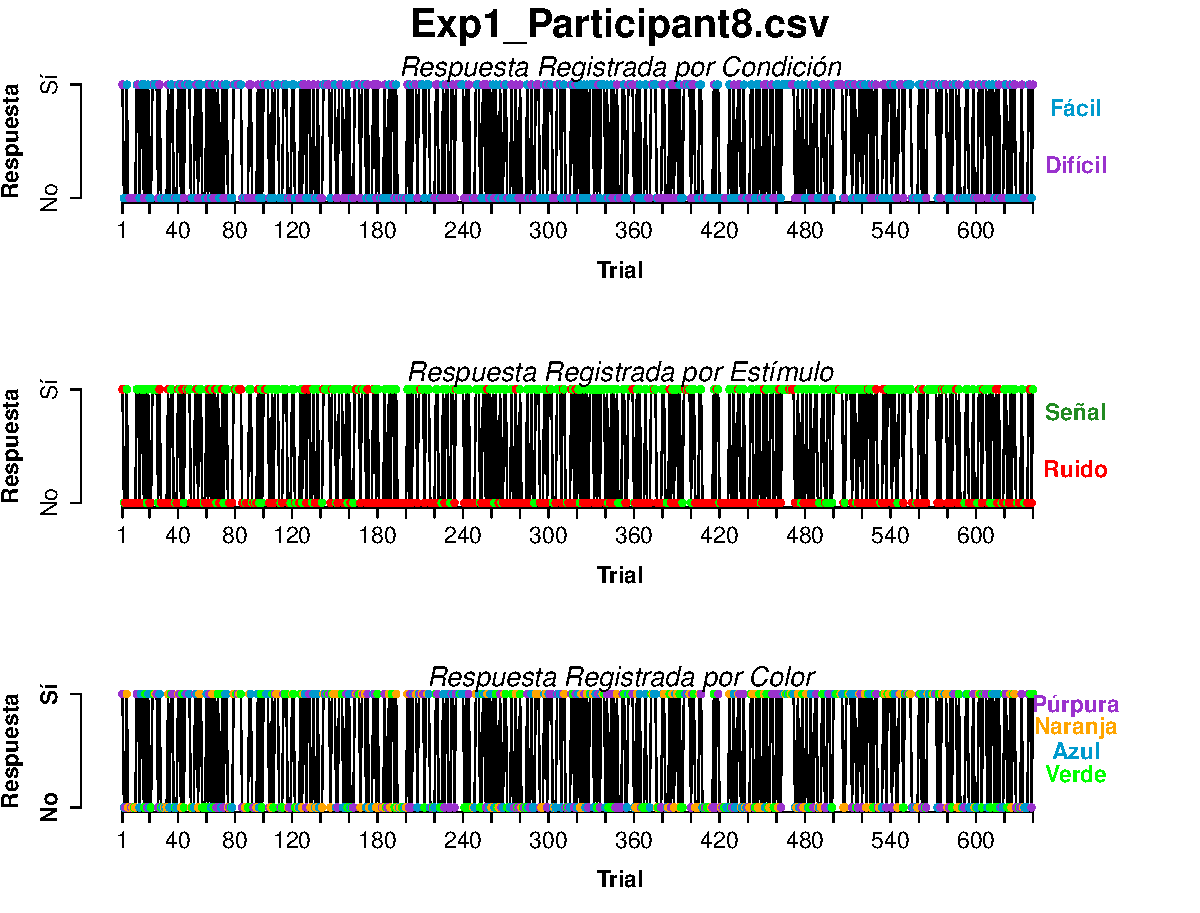
\includegraphics[width=0.30\textwidth]{Figures/BiasResp_Exp1_P8} 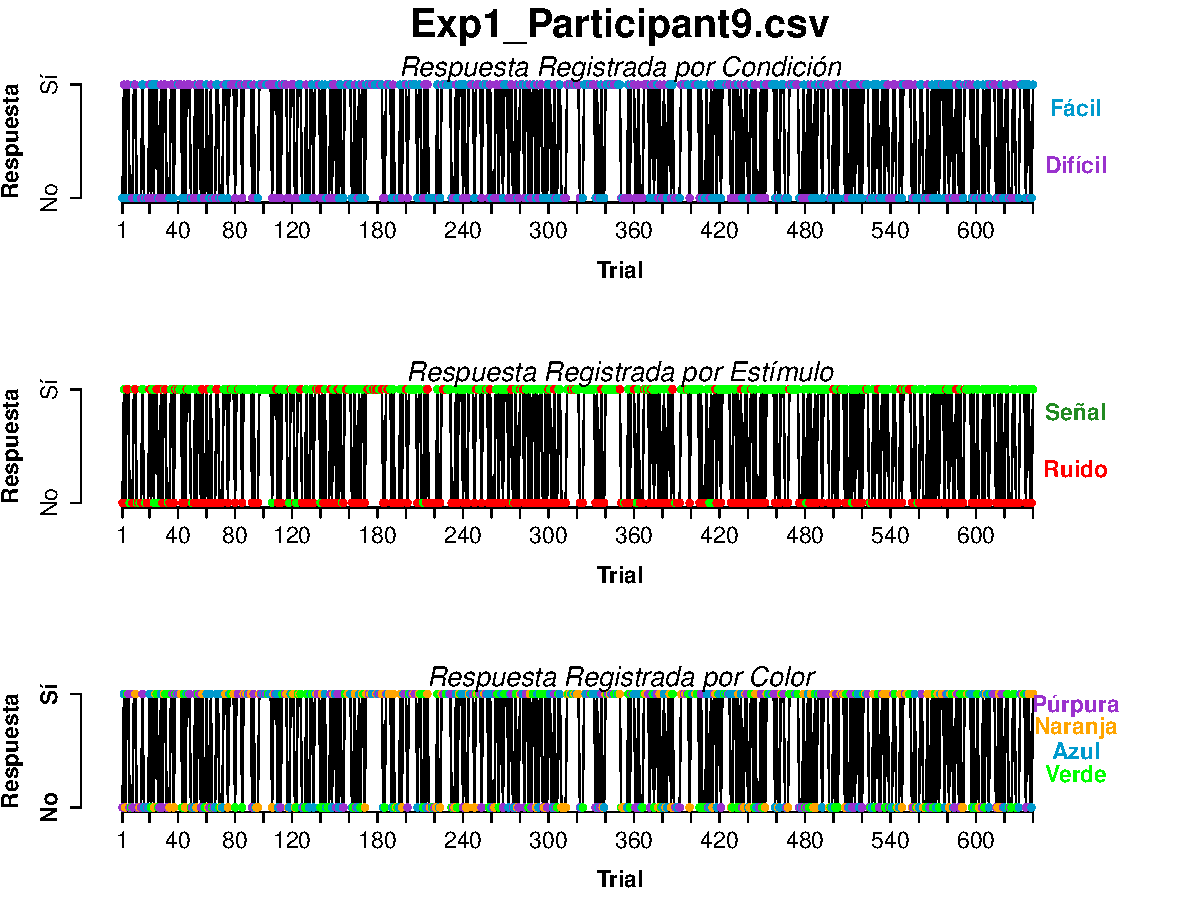
\includegraphics[width=0.30\textwidth]{Figures/BiasResp_Exp1_P9}
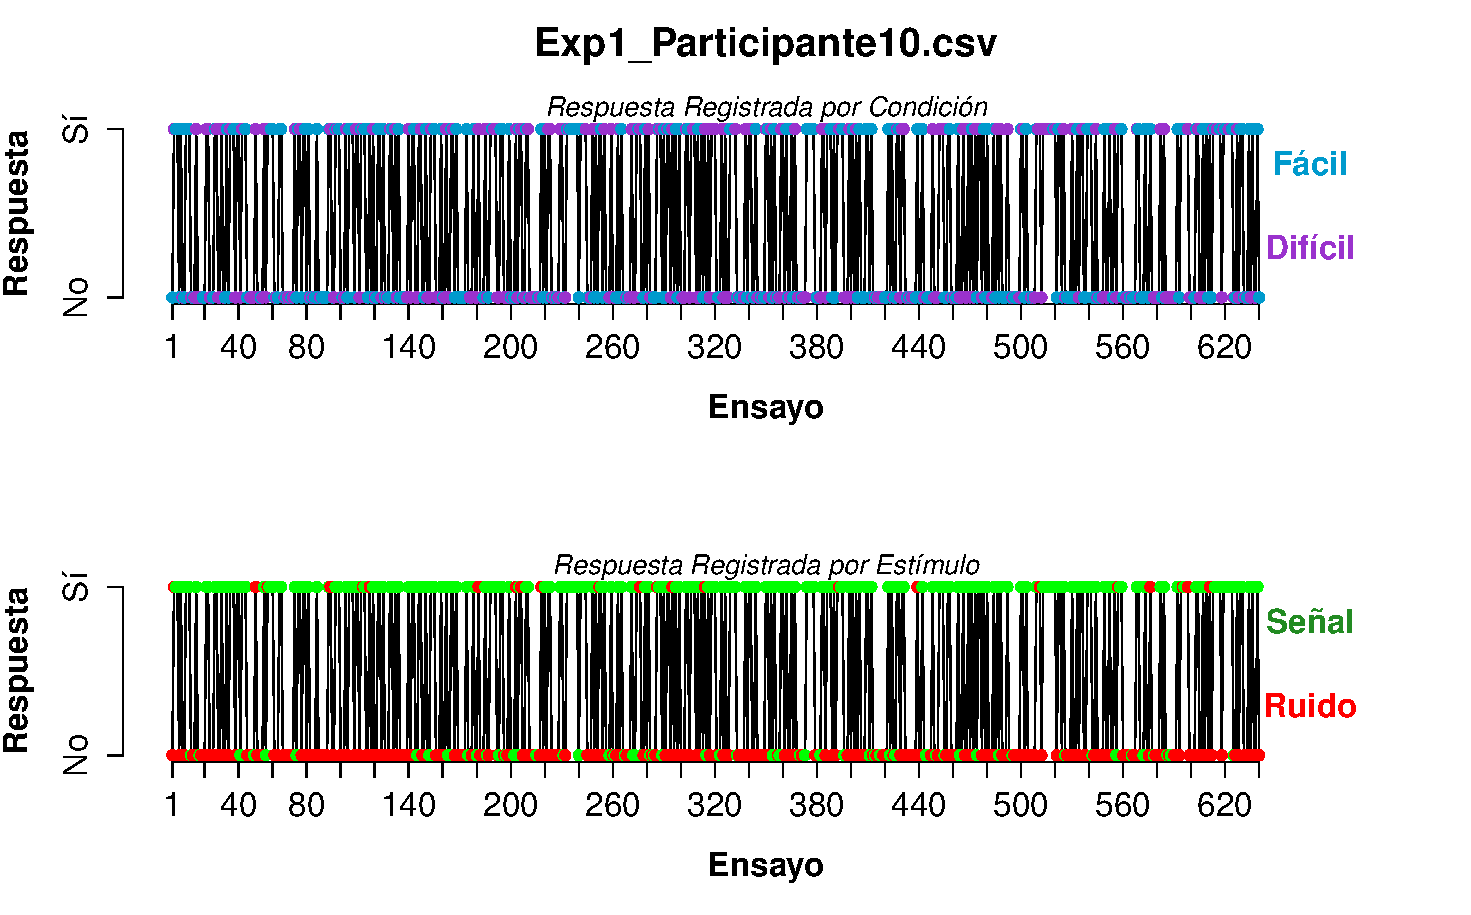
\includegraphics[width=0.30\textwidth]{Figures/BiasResp_Exp1_P10} 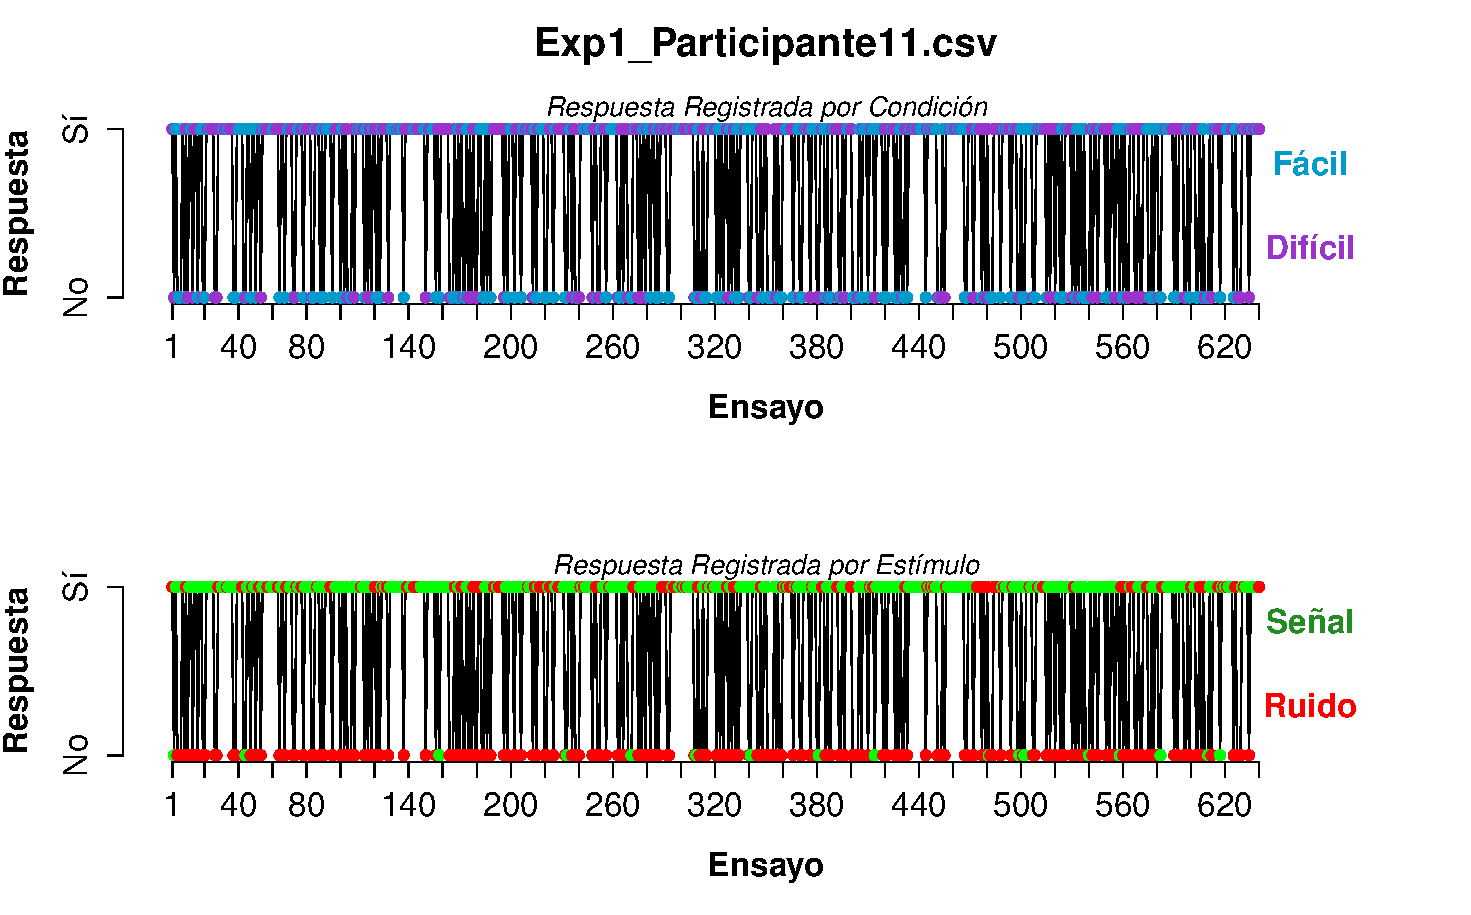
\includegraphics[width=0.30\textwidth]{Figures/BiasResp_Exp1_P11} 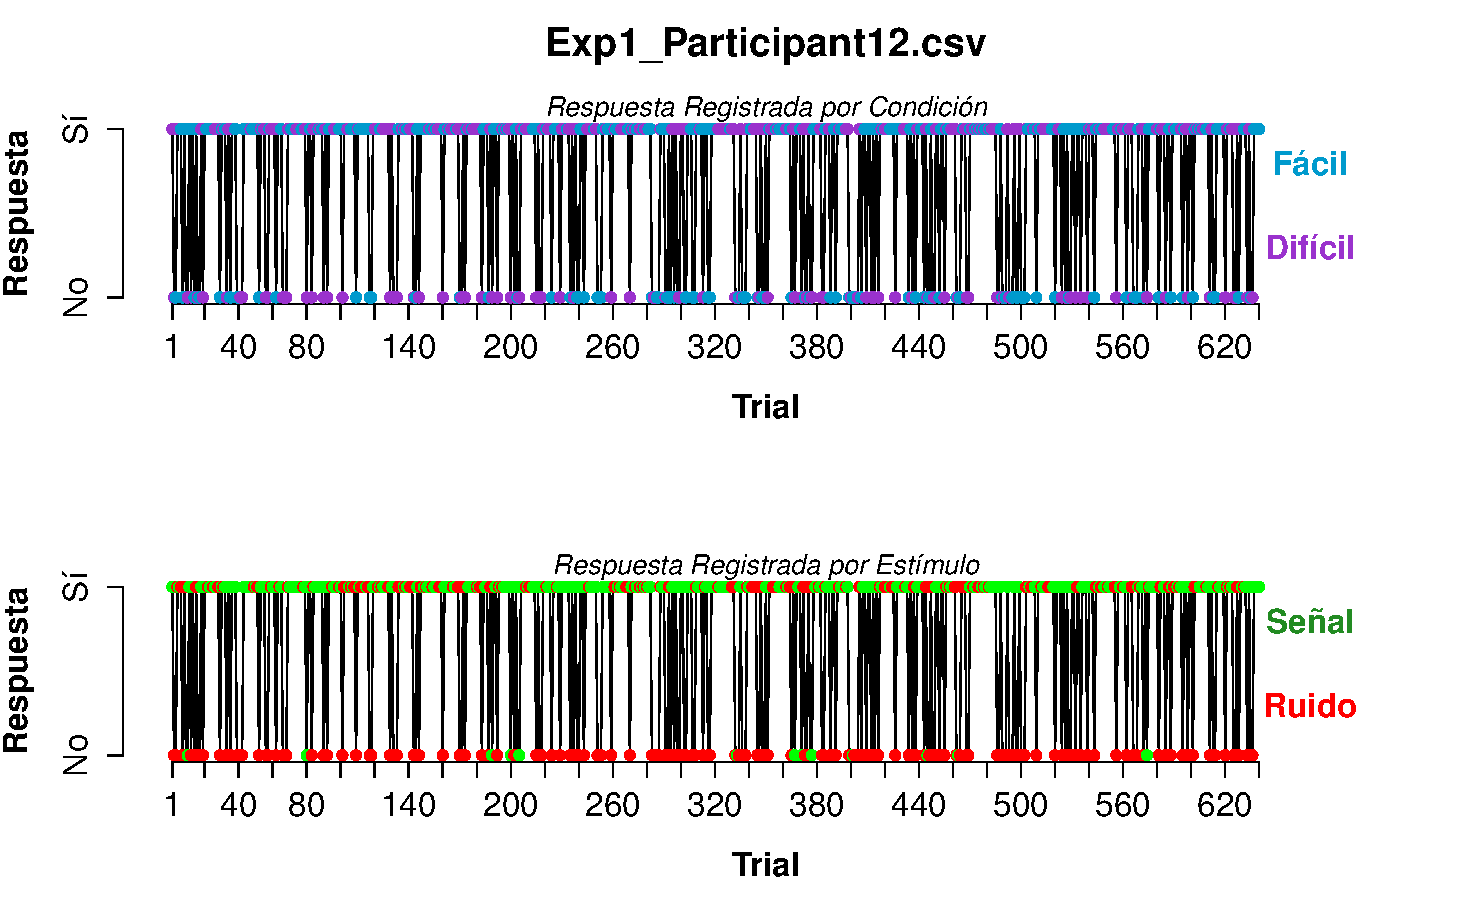
\includegraphics[width=0.30\textwidth]{Figures/BiasResp_Exp1_P12}
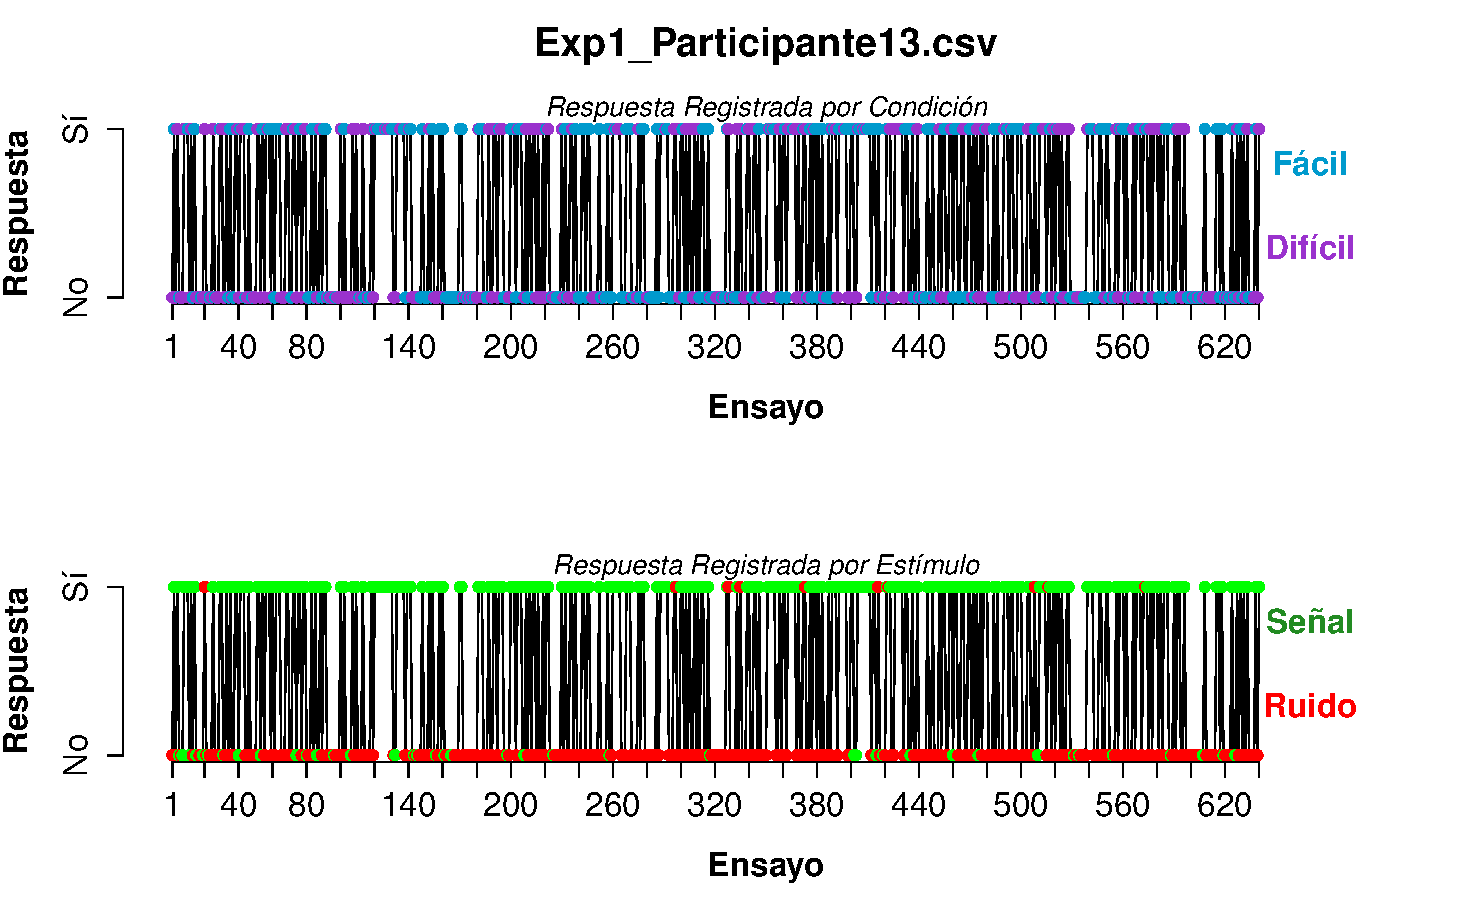
\includegraphics[width=0.30\textwidth]{Figures/BiasResp_Exp1_P13} 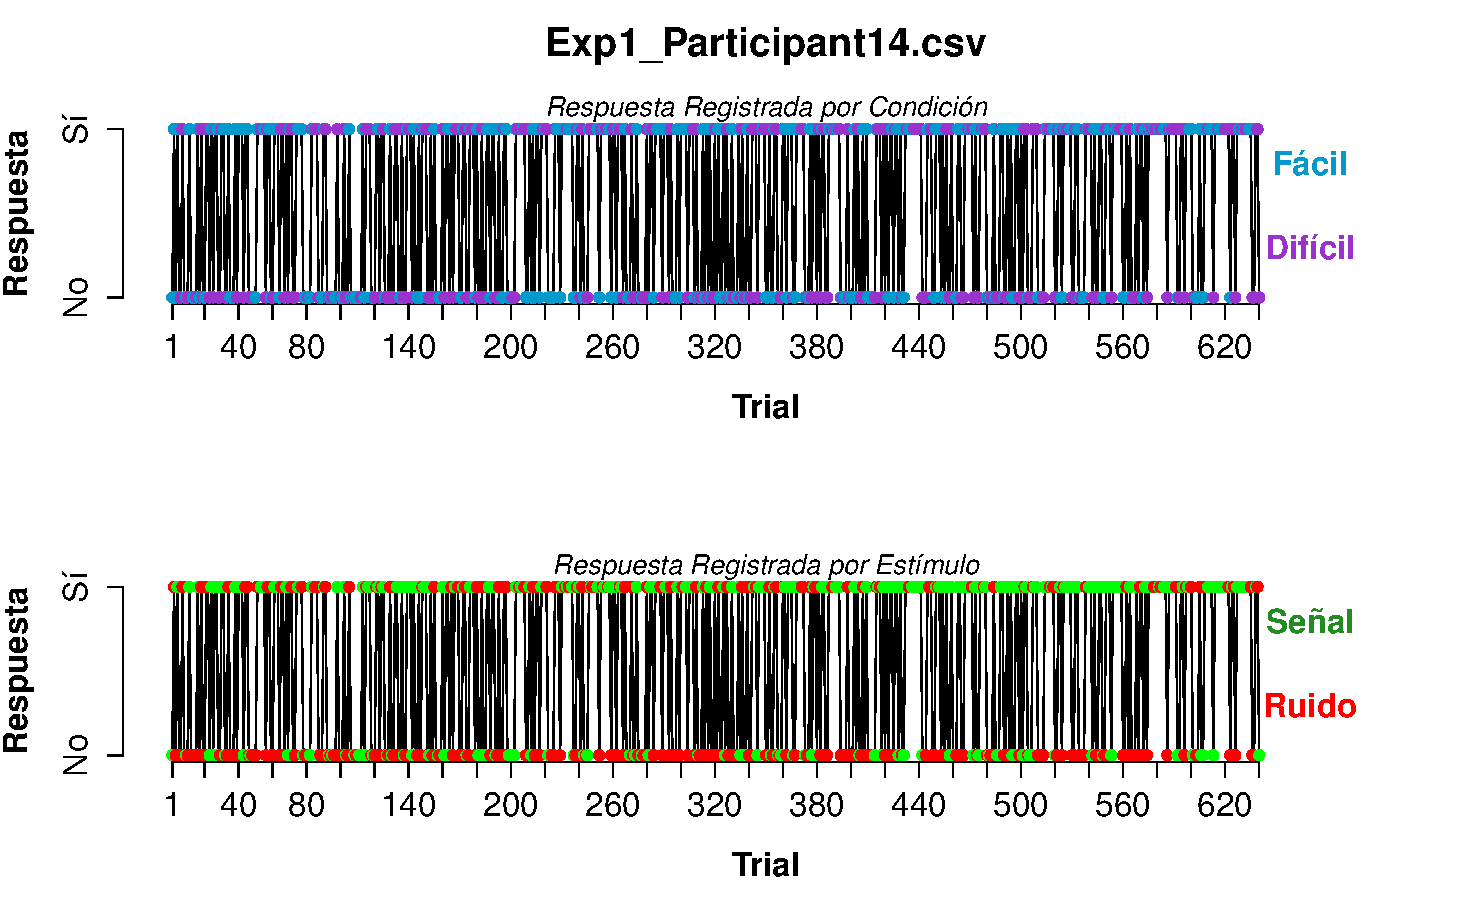
\includegraphics[width=0.30\textwidth]{Figures/BiasResp_Exp1_P14} 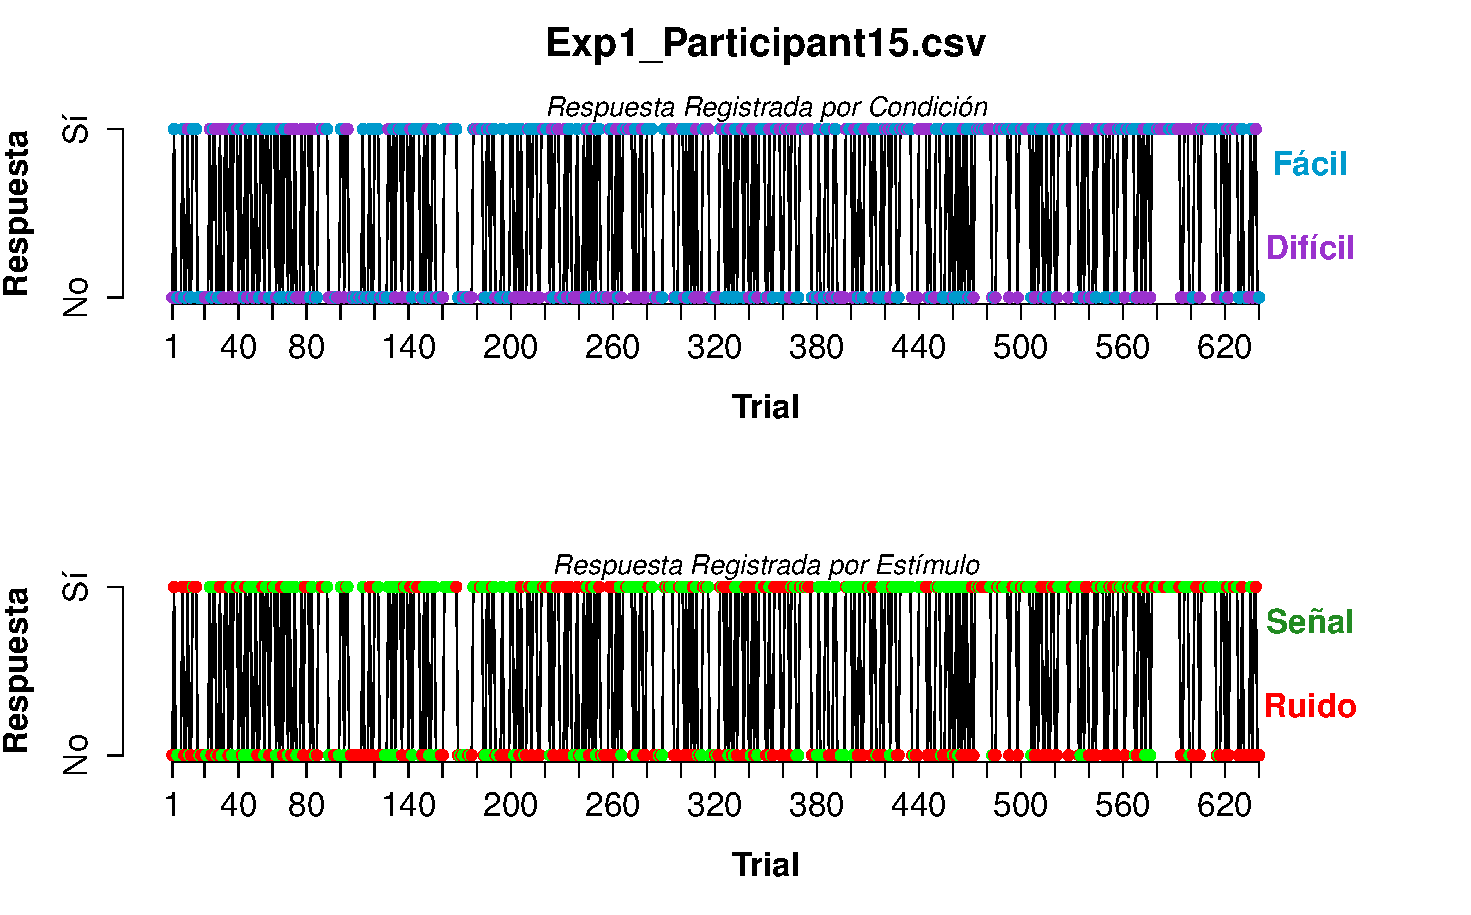
\includegraphics[width=0.30\textwidth]{Figures/BiasResp_Exp1_P15}
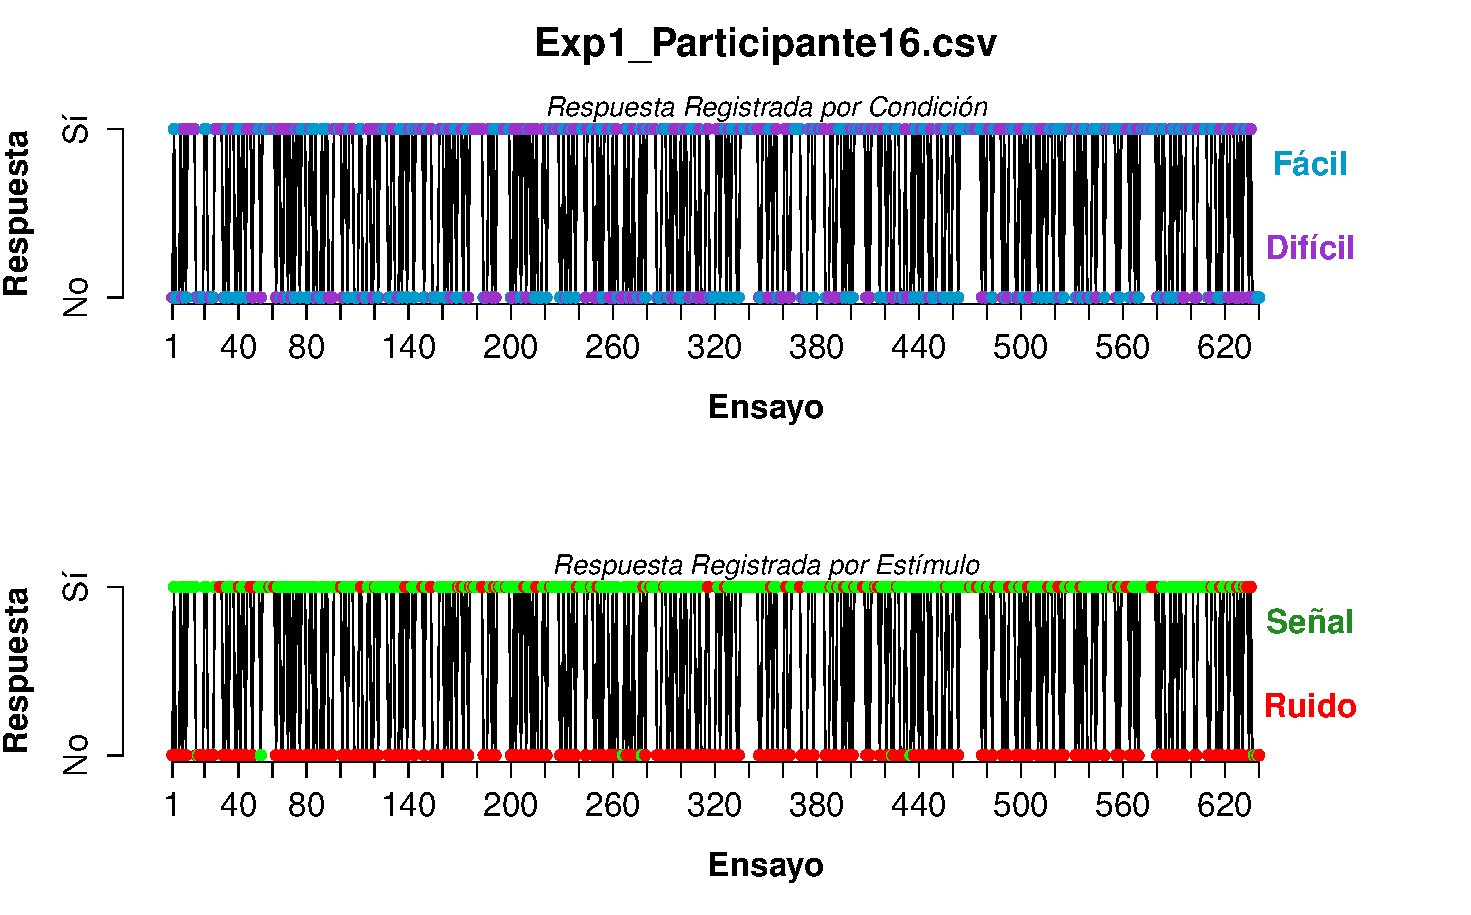
\includegraphics[width=0.30\textwidth]{Figures/BiasResp_Exp1_P16} 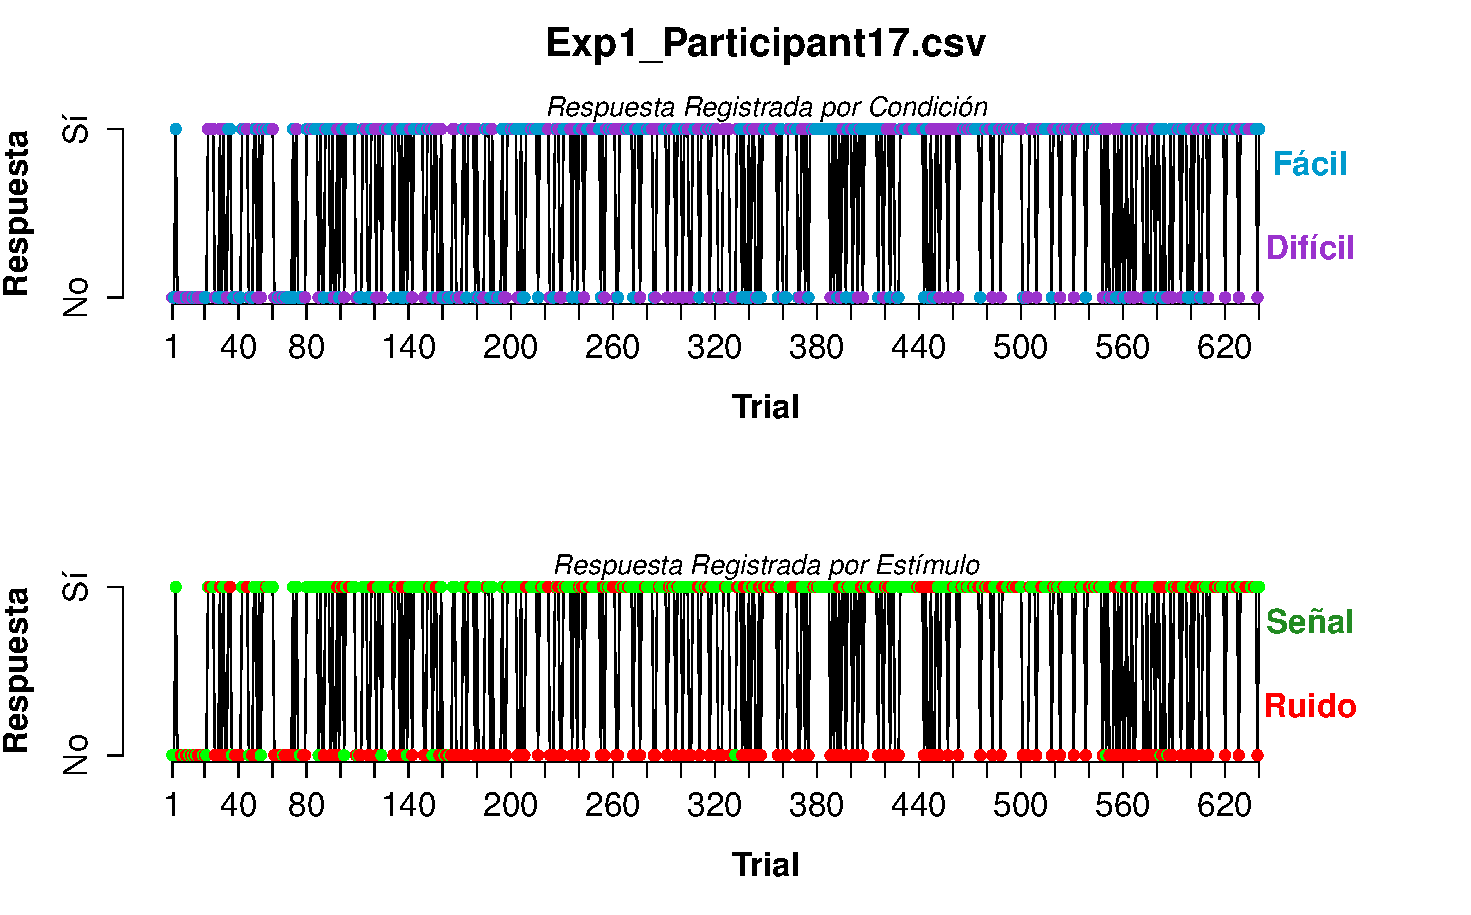
\includegraphics[width=0.30\textwidth]{Figures/BiasResp_Exp1_P17} 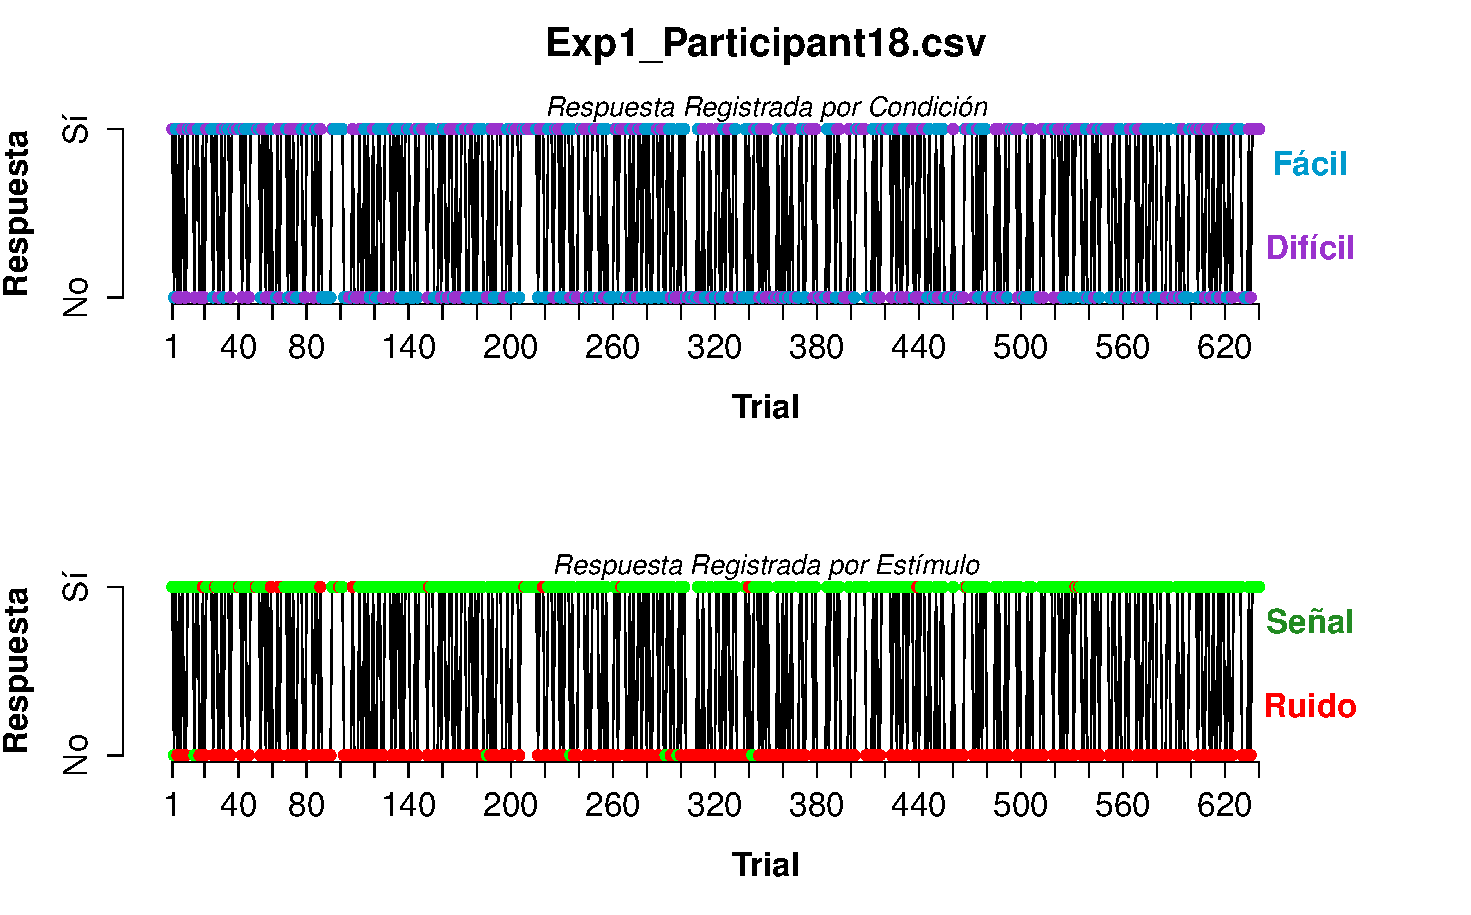
\includegraphics[width=0.30\textwidth]{Figures/BiasResp_Exp1_P18}
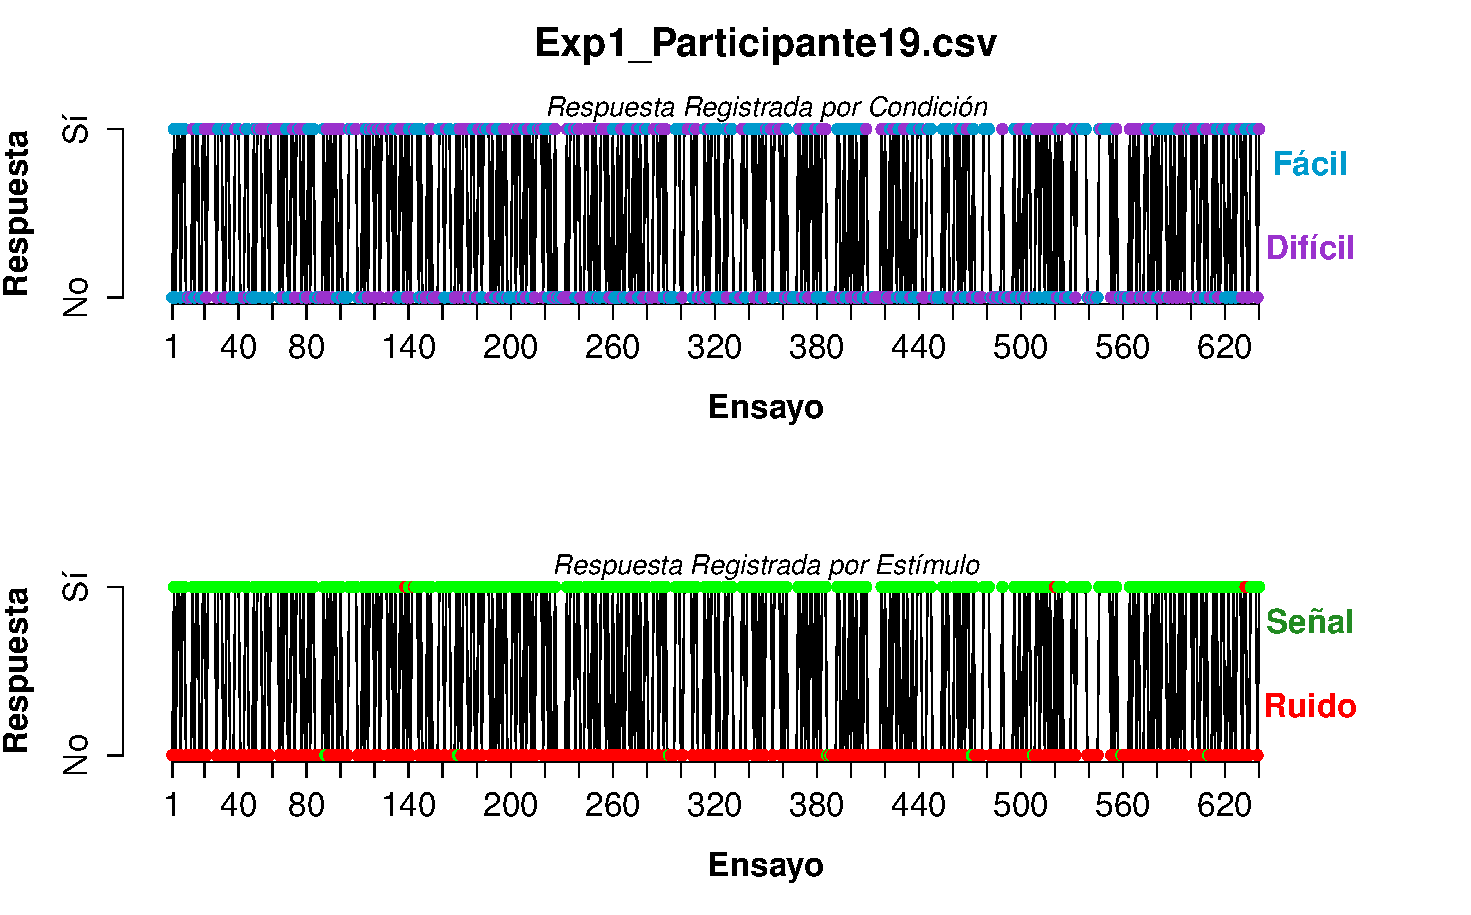
\includegraphics[width=0.30\textwidth]{Figures/BiasResp_Exp1_P19} 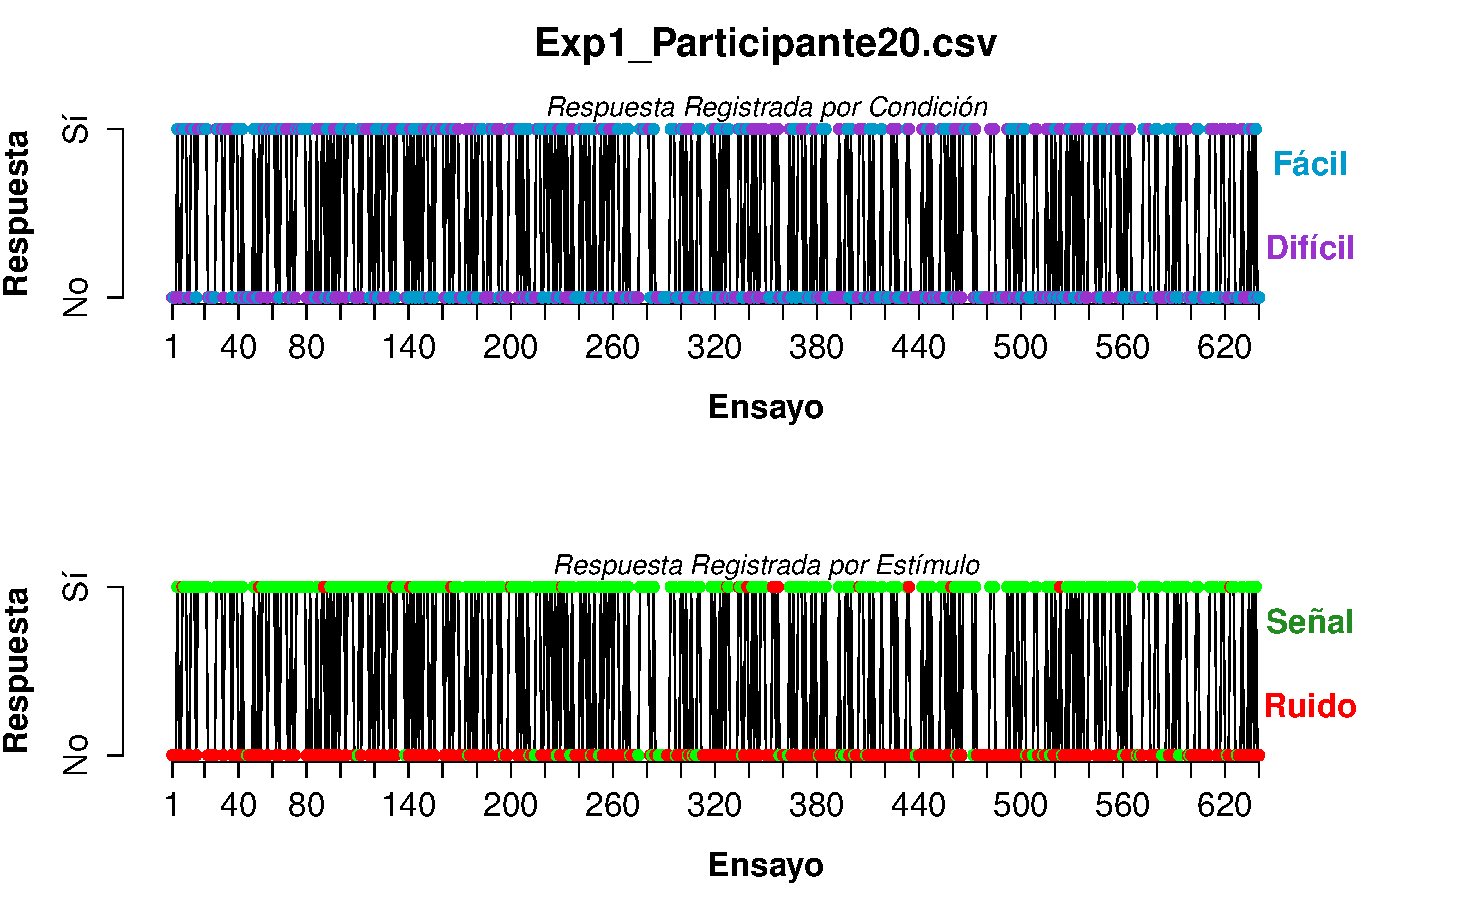
\includegraphics[width=0.30\textwidth]{Figures/BiasResp_Exp1_P20} 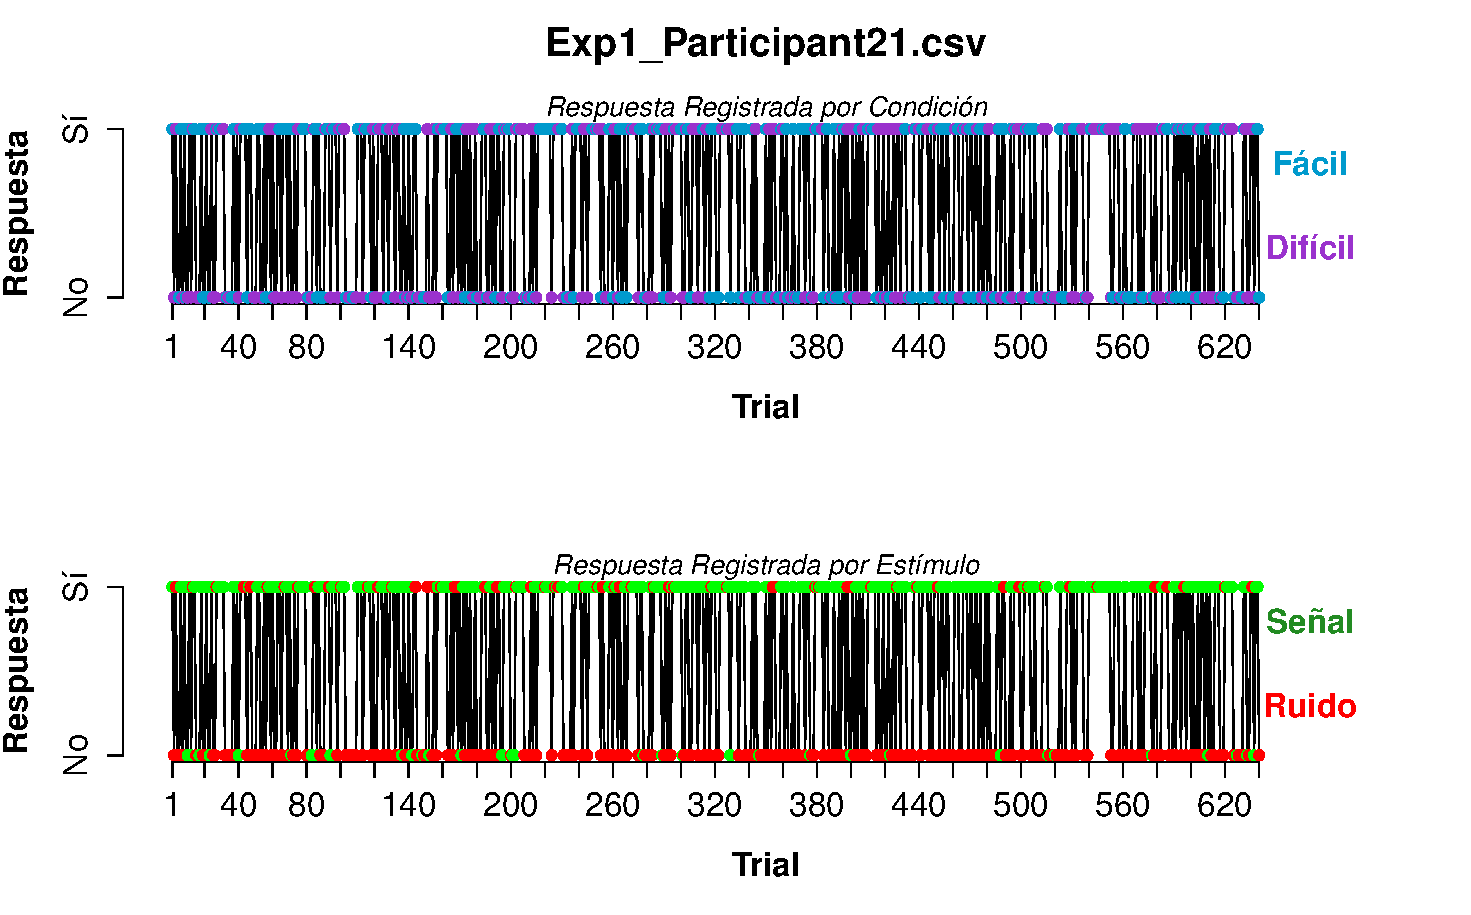
\includegraphics[width=0.30\textwidth]{Figures/BiasResp_Exp1_P21}
%\decoRule
\caption[Sesgo al Responder _Ex1]{Respuesta registrada por cada ensayo, con información adicional sobre el tipo de ensayo (Condición fácil o difícil (gráfico superior); tipo de ensayo señal o ruido (gráfico intermedio); color en que se presentó el estímulo (gráfico inferior)), (Experimento 2).}
\label{fig:BiasResp_E1}
\end{figure}


\begin{figure}[th]
\centering
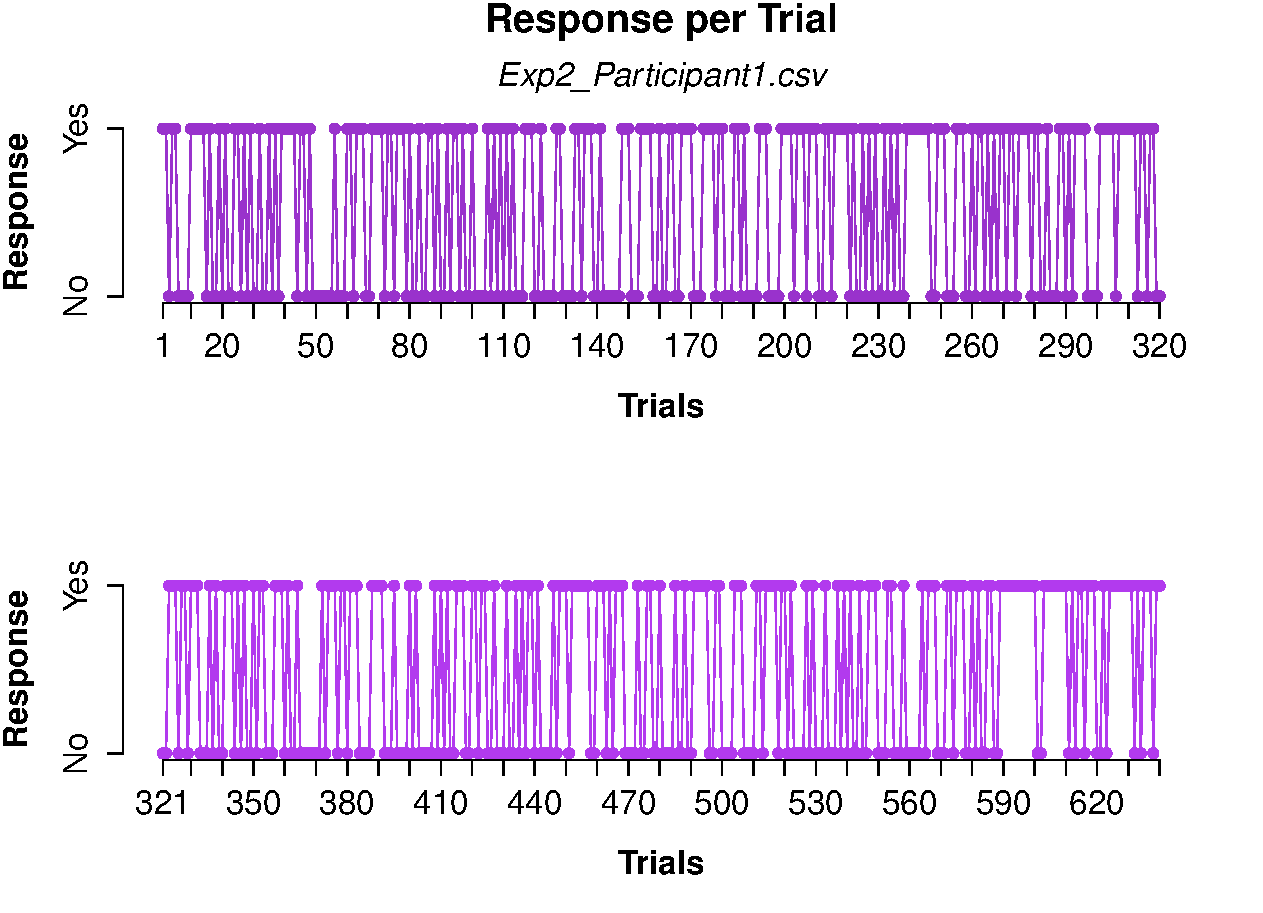
\includegraphics[width=0.30\textwidth]{Figures/Response_Exp2_P1} 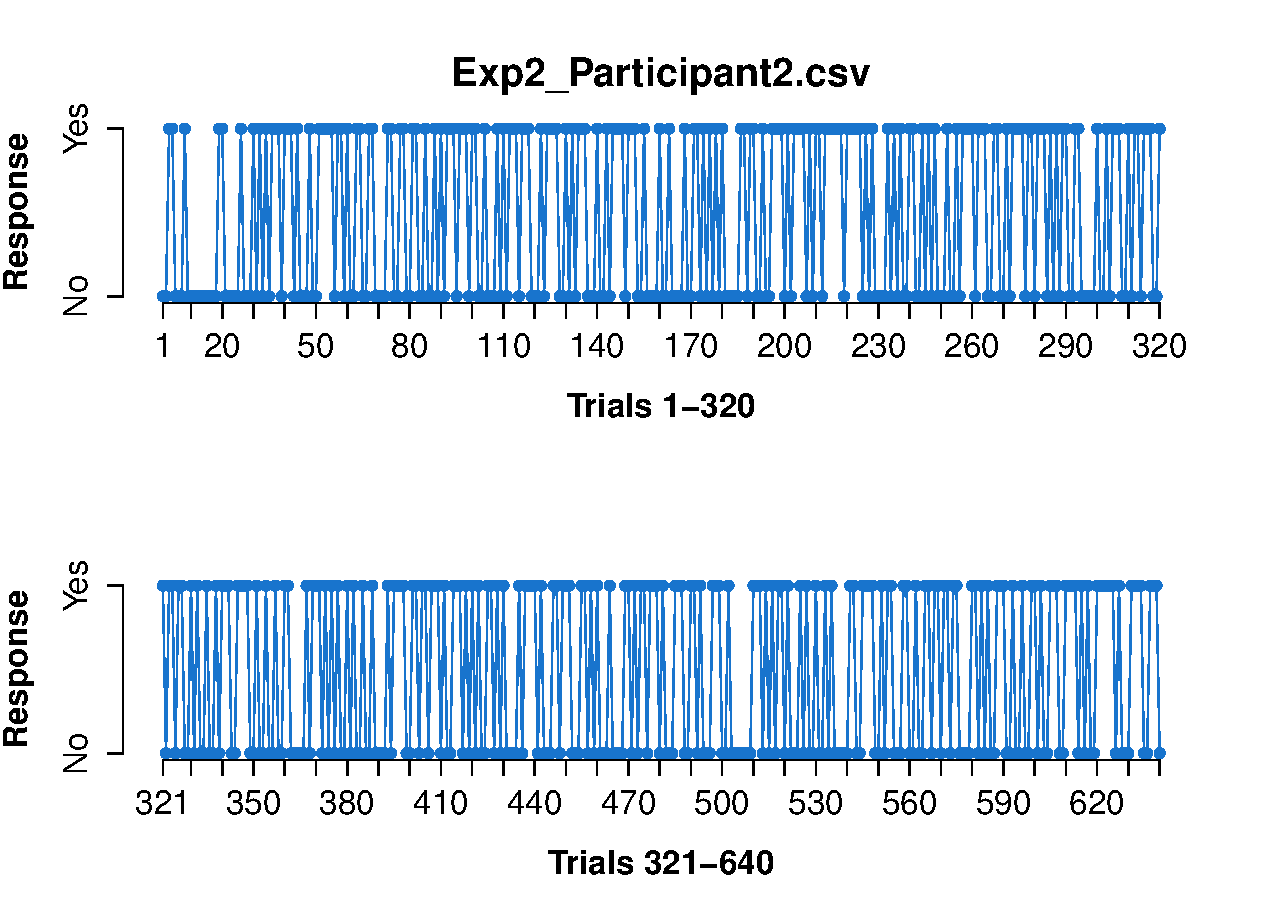
\includegraphics[width=0.30\textwidth]{Figures/Response_Exp2_P2} 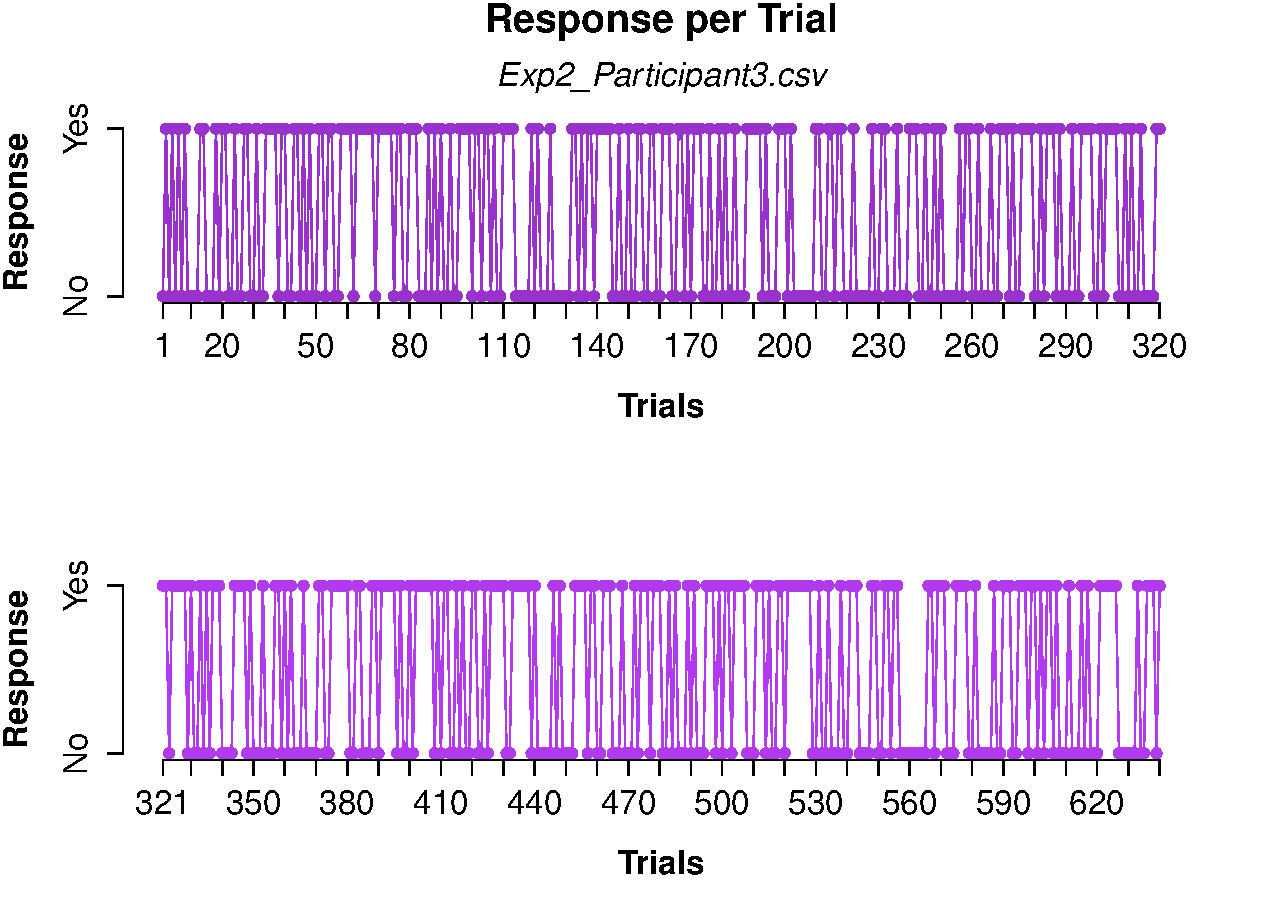
\includegraphics[width=0.30\textwidth]{Figures/Response_Exp2_P3}
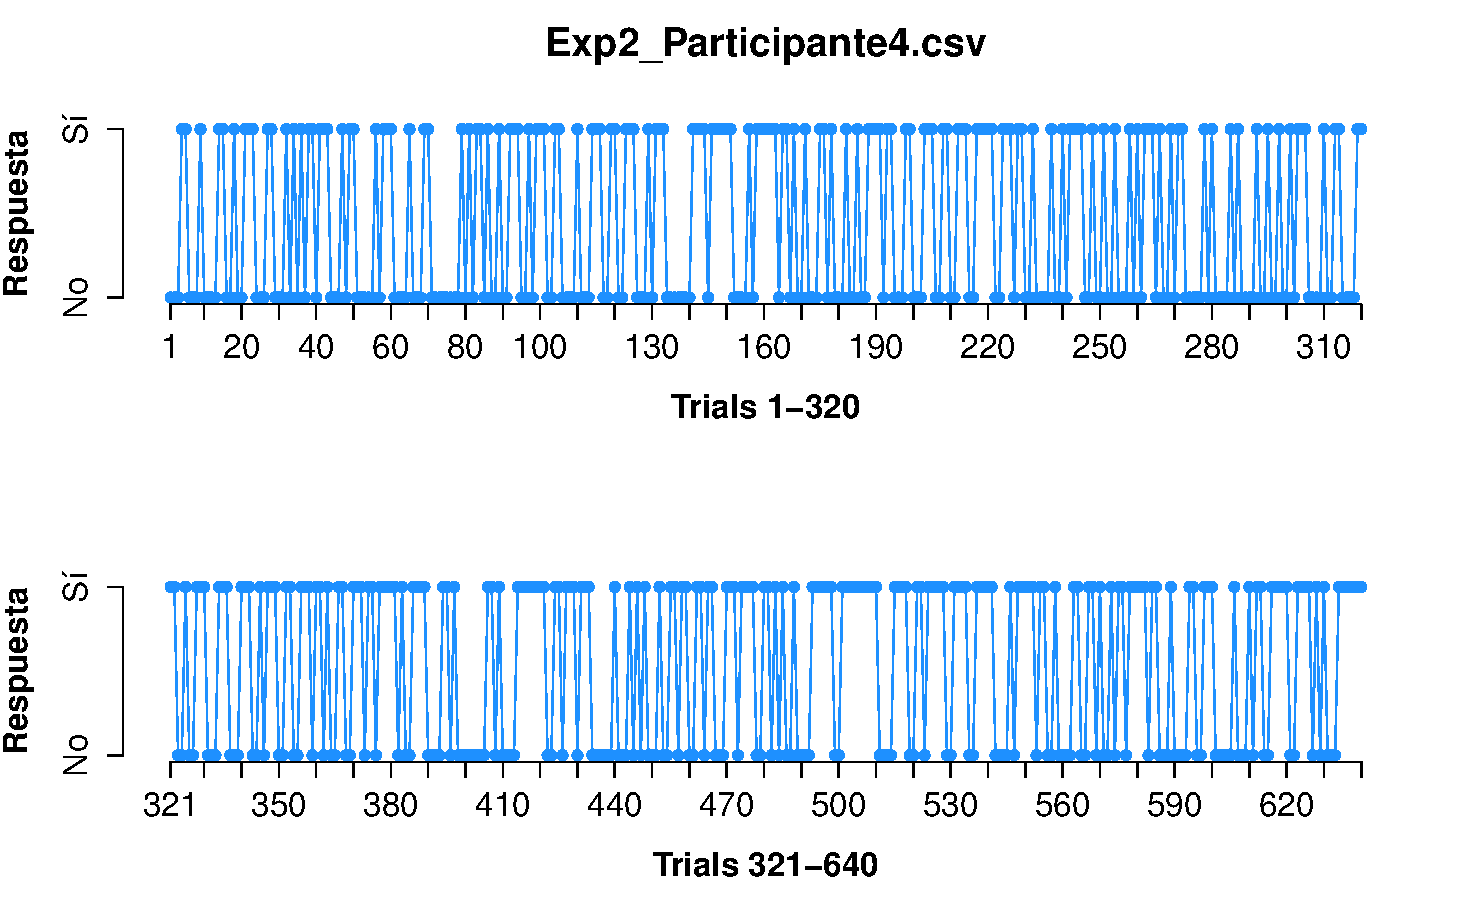
\includegraphics[width=0.30\textwidth]{Figures/Response_Exp2_P4} 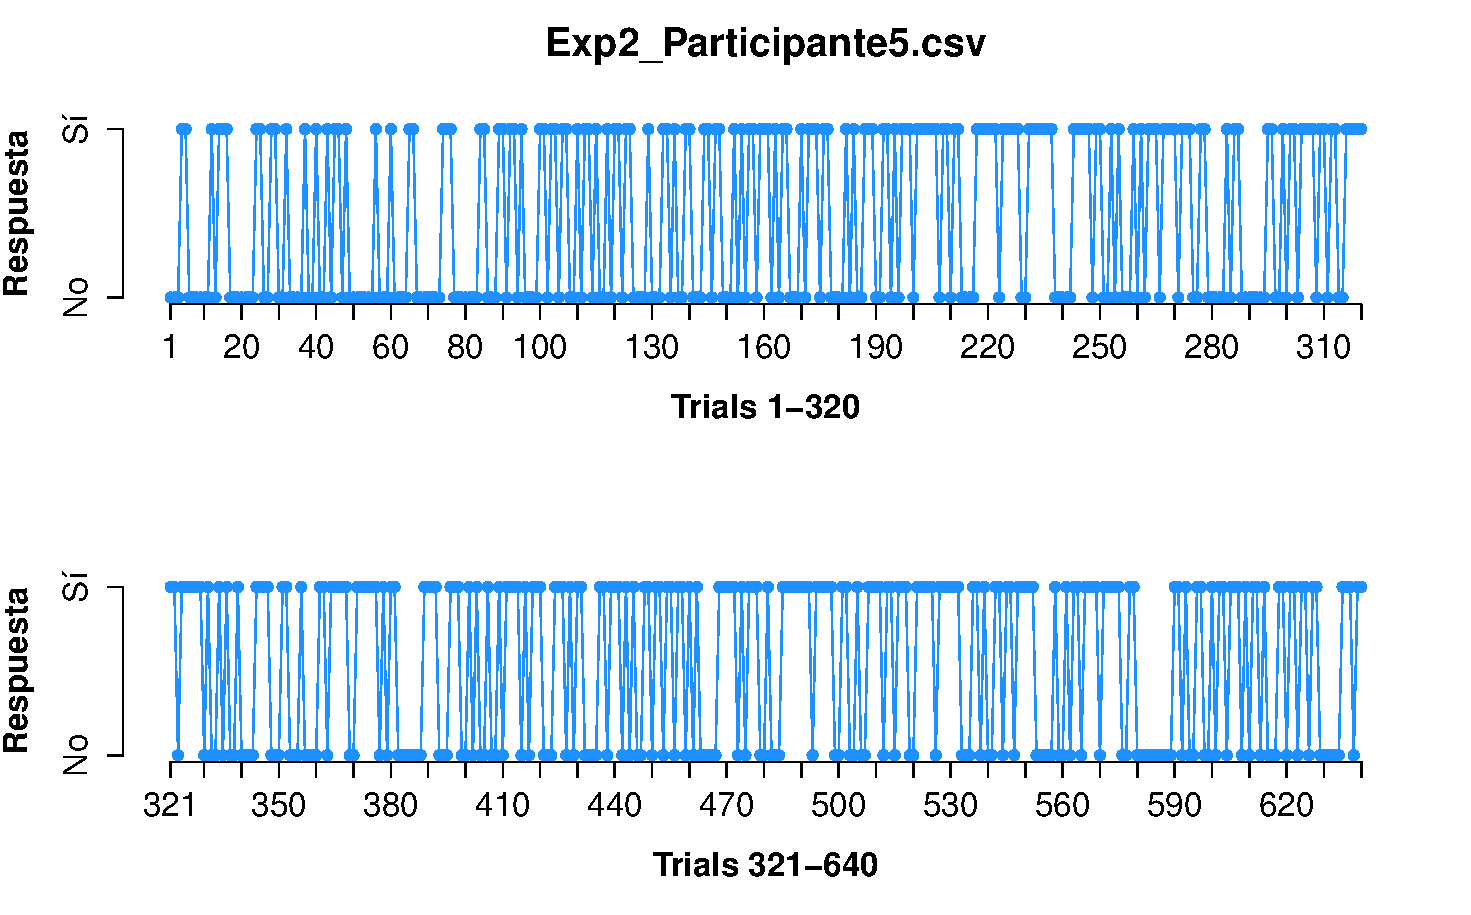
\includegraphics[width=0.30\textwidth]{Figures/Response_Exp2_P5} 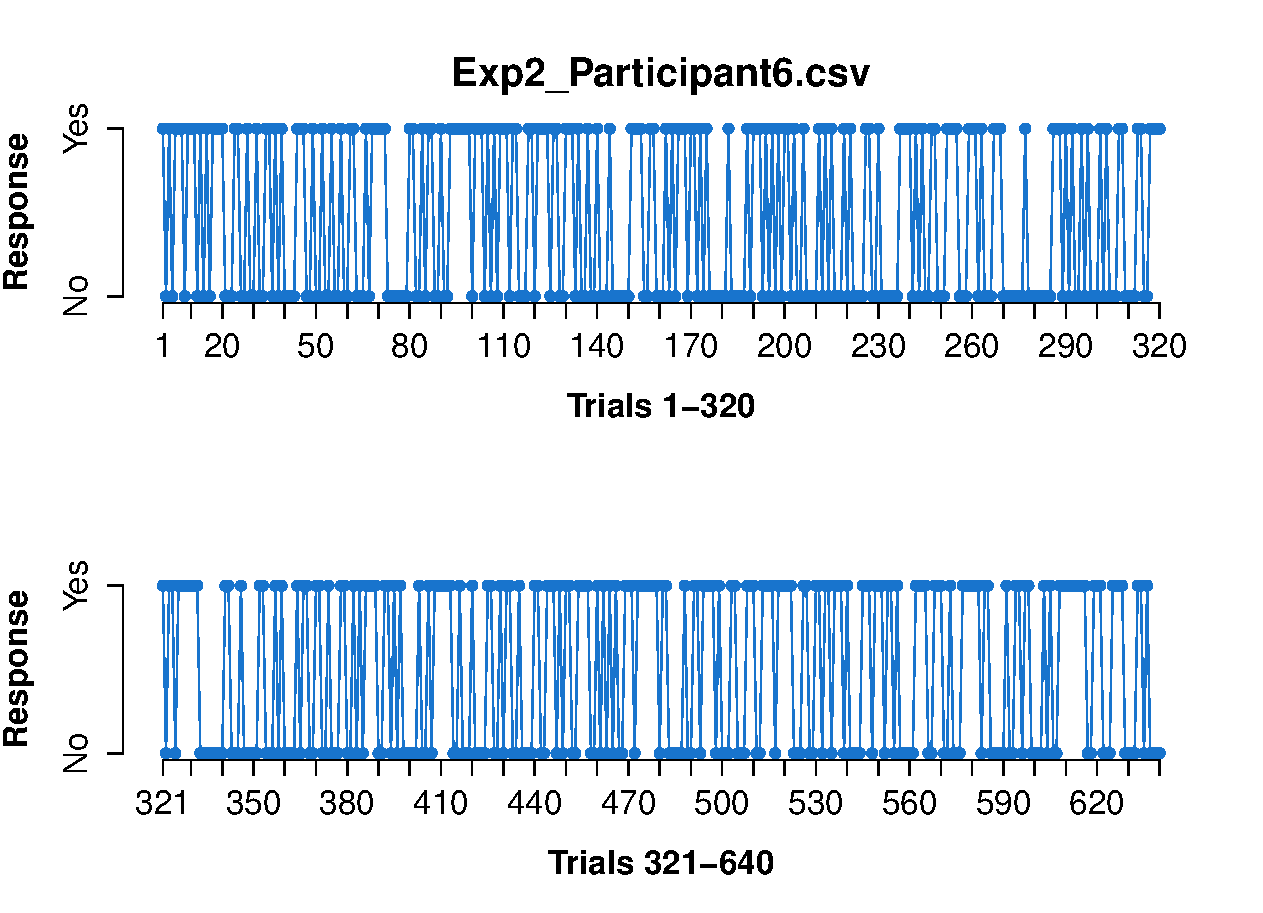
\includegraphics[width=0.30\textwidth]{Figures/Response_Exp2_P6}
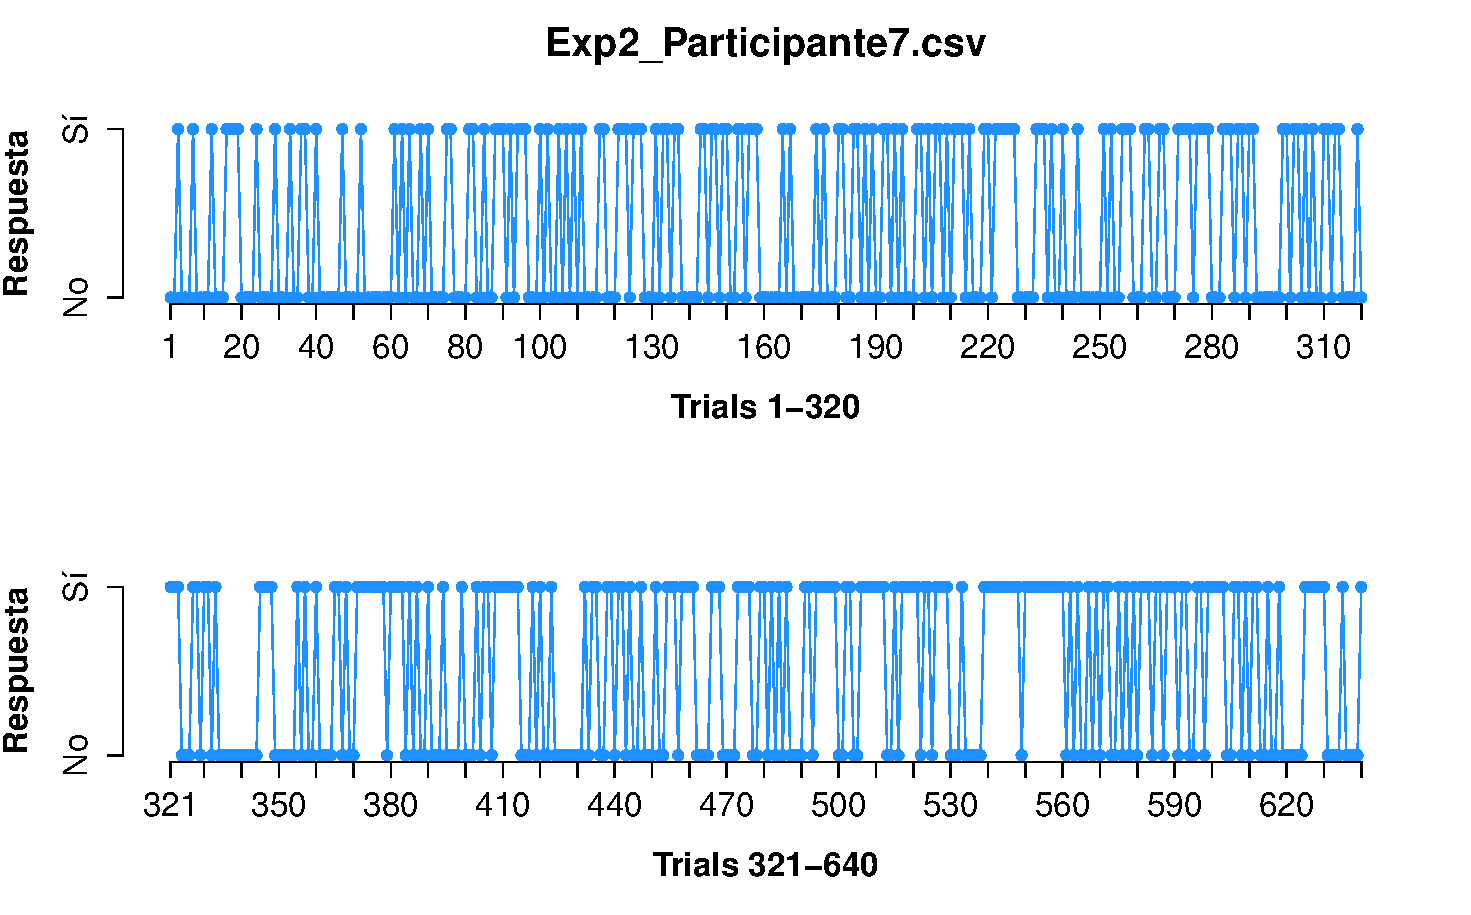
\includegraphics[width=0.30\textwidth]{Figures/Response_Exp2_P7} 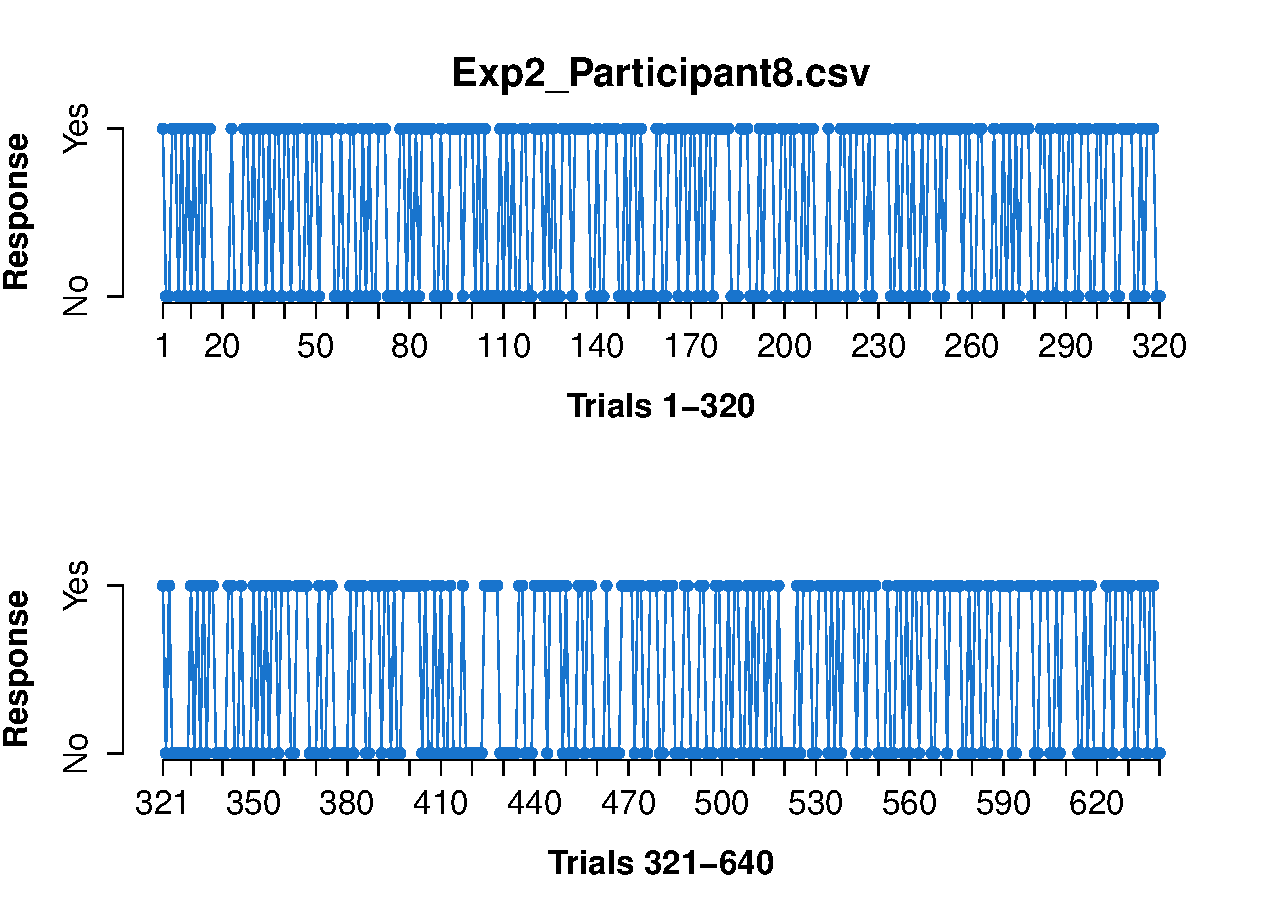
\includegraphics[width=0.30\textwidth]{Figures/Response_Exp2_P8} \includegraphics[width=0.30\textwidth]{Figures/Response_Exp2_P9}
\includegraphics[width=0.30\textwidth]{Figures/Response_Exp2_P10} \includegraphics[width=0.30\textwidth]{Figures/Response_Exp2_P11} \includegraphics[width=0.30\textwidth]{Figures/Response_Exp2_P12}
\includegraphics[width=0.30\textwidth]{Figures/Response_Exp2_P13} \includegraphics[width=0.30\textwidth]{Figures/Response_Exp2_P14} \includegraphics[width=0.30\textwidth]{Figures/Response_Exp2_P15}
\includegraphics[width=0.30\textwidth]{Figures/Response_Exp2_P16} \includegraphics[width=0.30\textwidth]{Figures/Response_Exp2_P17} \includegraphics[width=0.30\textwidth]{Figures/Response_Exp2_P18}
\includegraphics[width=0.30\textwidth]{Figures/Response_Exp2_P19} \includegraphics[width=0.30\textwidth]{Figures/Response_Exp2_P20} 
%\decoRule
\caption[Response_Exp2]{Respuesta registrada por cada ensayo (Experimento 2).}
\label{fig:Response_E2}
\end{figure}



%%%%%%%%%%%%%%%%%%%%%%%%%%%%%%%%%%%%%%%%%%%%%%%%%%%%%%%%%%%%%%
%%%%%%%%%  Respuesta Rating en los ensayos
% Experimento 2
%%%%%%%%%%%%%%%%%%%%%%%%%%%%%%%%%%%%%%%%%%%%%%%%%%%%%%%%%%%%%%%
\begin{figure}[th]
\centering
\includegraphics[width=0.30\textwidth]{Figures/Rating_Exp2_P1} \includegraphics[width=0.30\textwidth]{Figures/Rating_Exp2_P2} \includegraphics[width=0.30\textwidth]{Figures/Rating_Exp2_P3}
\includegraphics[width=0.30\textwidth]{Figures/Rating_Exp2_P4} \includegraphics[width=0.30\textwidth]{Figures/Rating_Exp2_P5} \includegraphics[width=0.30\textwidth]{Figures/Rating_Exp2_P6}
\includegraphics[width=0.30\textwidth]{Figures/Rating_Exp2_P7} \includegraphics[width=0.30\textwidth]{Figures/Rating_Exp2_P8} \includegraphics[width=0.30\textwidth]{Figures/Rating_Exp2_P9}
\includegraphics[width=0.30\textwidth]{Figures/Rating_Exp2_P10} \includegraphics[width=0.30\textwidth]{Figures/Rating_Exp2_P11} \includegraphics[width=0.30\textwidth]{Figures/Rating_Exp2_P12}
\includegraphics[width=0.30\textwidth]{Figures/Rating_Exp2_P13} \includegraphics[width=0.30\textwidth]{Figures/Rating_Exp2_P14} \includegraphics[width=0.30\textwidth]{Figures/Rating_Exp2_P15}
\includegraphics[width=0.30\textwidth]{Figures/Rating_Exp2_P16} \includegraphics[width=0.30\textwidth]{Figures/Rating_Exp2_P17} \includegraphics[width=0.30\textwidth]{Figures/Rating_Exp2_P18}
\includegraphics[width=0.30\textwidth]{Figures/Rating_Exp2_P19} \includegraphics[width=0.30\textwidth]{Figures/Rating_Exp2_P20} 
%\decoRule
\caption[Rating_Exp2]{Puntaje asignado a a Escala de Confianza por cada ensayo (Experimento 2).}
\label{fig:Rating_E2}
\end{figure}




\subsection{Control 2: Evaluando tiempos de respuesta a lo largo del experimento}


%%%%%%%%%%%%%%%%%%%%%%%%%%%%%%%%%%%%%%%%%%%%%%%%%%%%%%%%%%%%%%
%%%%%%%%%  Respuesta Rating en los ensayos
% Experimento 2
%%%%%%%%%%%%%%%%%%%%%%%%%%%%%%%%%%%%%%%%%%%%%%%%%%%%%%%%%%%%%%%
\begin{figure}[th]
\centering
\includegraphics[width=0.30\textwidth]{Figures/RTs_Exp2_P1} \includegraphics[width=0.30\textwidth]{Figures/RTs_Exp2_P2} \includegraphics[width=0.30\textwidth]{Figures/RTs_Exp2_P3}
\includegraphics[width=0.30\textwidth]{Figures/RTs_Exp2_P4} \includegraphics[width=0.30\textwidth]{Figures/RTs_Exp2_P5} \includegraphics[width=0.30\textwidth]{Figures/RTs_Exp2_P6}
\includegraphics[width=0.30\textwidth]{Figures/RTs_Exp2_P7} \includegraphics[width=0.30\textwidth]{Figures/RTs_Exp2_P8} \includegraphics[width=0.30\textwidth]{Figures/RTs_Exp2_P9}
\includegraphics[width=0.30\textwidth]{Figures/RTs_Exp2_P10} \includegraphics[width=0.30\textwidth]{Figures/RTs_Exp2_P11} \includegraphics[width=0.30\textwidth]{Figures/RTs_Exp2_P12}
\includegraphics[width=0.30\textwidth]{Figures/RTs_Exp2_P13} \includegraphics[width=0.30\textwidth]{Figures/RTs_Exp2_P14} \includegraphics[width=0.30\textwidth]{Figures/RTs_Exp2_P15}
\includegraphics[width=0.30\textwidth]{Figures/RTs_Exp2_P16} \includegraphics[width=0.30\textwidth]{Figures/RTs_Exp2_P17} \includegraphics[width=0.30\textwidth]{Figures/RTs_Exp2_P18}
\includegraphics[width=0.30\textwidth]{Figures/RTs_Exp2_P19} \includegraphics[width=0.30\textwidth]{Figures/RTs_Exp2_P20} 
%\decoRule
\caption[TRs_Exp2]{Tiempos de Respuesta por ensayo (Experimento 2). Se muestran simultáneamente el tiempo de respuesta a la tarea principal (Color X) y a la escala de confianza (Color Y).}
\label{fig:RTs_E2}
\end{figure}


%%%%%%%%%%%%%%%%%%%%%%%%%%%%%%%%%%%%%%%%%%%%%%%%%%%%%%%%%%%%%%
%%%%%%%%%  Respuesta Rating en los ensayos
% Experimento 2
%%%%%%%%%%%%%%%%%%%%%%%%%%%%%%%%%%%%%%%%%%%%%%%%%%%%%%%%%%%%%%%
\begin{figure}[th]
\centering
\includegraphics[width=0.30\textwidth]{Figures/RT1_Exp2_P1} \includegraphics[width=0.30\textwidth]{Figures/RT1_Exp2_P2} \includegraphics[width=0.30\textwidth]{Figures/RT1_Exp2_P3}
\includegraphics[width=0.30\textwidth]{Figures/RT1_Exp2_P4} \includegraphics[width=0.30\textwidth]{Figures/RT1_Exp2_P5} \includegraphics[width=0.30\textwidth]{Figures/RT1_Exp2_P6}
\includegraphics[width=0.30\textwidth]{Figures/RT1_Exp2_P7} \includegraphics[width=0.30\textwidth]{Figures/RT1_Exp2_P8} \includegraphics[width=0.30\textwidth]{Figures/RT1_Exp2_P9}
\includegraphics[width=0.30\textwidth]{Figures/RT1_Exp2_P10} \includegraphics[width=0.30\textwidth]{Figures/RT1_Exp2_P11} \includegraphics[width=0.30\textwidth]{Figures/RT1_Exp2_P12}
\includegraphics[width=0.30\textwidth]{Figures/RT1_Exp2_P13} \includegraphics[width=0.30\textwidth]{Figures/RT1_Exp2_P14} \includegraphics[width=0.30\textwidth]{Figures/RT1_Exp2_P15}
\includegraphics[width=0.30\textwidth]{Figures/RT1_Exp2_P16} \includegraphics[width=0.30\textwidth]{Figures/RT1_Exp2_P17} \includegraphics[width=0.30\textwidth]{Figures/RT1_Exp2_P18}
\includegraphics[width=0.30\textwidth]{Figures/RT1_Exp2_P19} \includegraphics[width=0.30\textwidth]{Figures/RT1_Exp2_P20} 
%\decoRule
\caption[TR1_Exp2]{Tiempo de Respuesta a la tarea perceptual por ensayo (Experimento 2).}
\label{fig:RT1_E2}
\end{figure}


%%%%%%%%%%%%%%%%%%%%%%%%%%%%%%%%%%%%%%%%%%%%%%%%%%%%%%%%%%%%%%
%%%%%%%%%  Respuesta Rating en los ensayos
% Experimento 2
%%%%%%%%%%%%%%%%%%%%%%%%%%%%%%%%%%%%%%%%%%%%%%%%%%%%%%%%%%%%%%%
\begin{figure}[th]
\centering
\includegraphics[width=0.30\textwidth]{Figures/RT2_Exp2_P1} \includegraphics[width=0.30\textwidth]{Figures/RT2_Exp2_P2} \includegraphics[width=0.30\textwidth]{Figures/RT2_Exp2_P3}
\includegraphics[width=0.30\textwidth]{Figures/RT2_Exp2_P4} \includegraphics[width=0.30\textwidth]{Figures/RT2_Exp2_P5} \includegraphics[width=0.30\textwidth]{Figures/RT2_Exp2_P6}
\includegraphics[width=0.30\textwidth]{Figures/RT2_Exp2_P7} \includegraphics[width=0.30\textwidth]{Figures/RT2_Exp2_P8} \includegraphics[width=0.30\textwidth]{Figures/RT2_Exp2_P9}
\includegraphics[width=0.30\textwidth]{Figures/RT2_Exp2_P10} \includegraphics[width=0.30\textwidth]{Figures/RT2_Exp2_P11} \includegraphics[width=0.30\textwidth]{Figures/RT2_Exp2_P12}
\includegraphics[width=0.30\textwidth]{Figures/RT2_Exp2_P13} \includegraphics[width=0.30\textwidth]{Figures/RT2_Exp2_P14} \includegraphics[width=0.30\textwidth]{Figures/RT2_Exp2_P15}
\includegraphics[width=0.30\textwidth]{Figures/RT2_Exp2_P16} \includegraphics[width=0.30\textwidth]{Figures/RT2_Exp2_P17} \includegraphics[width=0.30\textwidth]{Figures/RT2_Exp2_P18}
\includegraphics[width=0.30\textwidth]{Figures/RT2_Exp2_P19} \includegraphics[width=0.30\textwidth]{Figures/RT2_Exp2_P20} 
%\decoRule
\caption[TR2_Exp2]{Tiempo de respuesta a la escala de confianza por ensayo (Experimento 2).}
\label{fig:RT2_E2}
\end{figure}



\subsection{Control 3: ¿La duración del experimento tuvo un impacto en la ejecución de los participantes?}


%%%%%%%%%%%%%%%%%%%%%%%%%%%%%%%%%%%%%%%%%%%%%%%%%%%%%%%%%%%%%%
%%%%%%%%%  Respuesta (Y/N) en los ensayos
% Experimento 2
%%%%%%%%%%%%%%%%%%%%%%%%%%%%%%%%%%%%%%%%%%%%%%%%%%%%%%%%%%%%%%%
\begin{figure}[th]
\centering
\includegraphics[width=0.30\textwidth]{Figures/Success_Exp1_P1} \includegraphics[width=0.30\textwidth]{Figures/Success_Exp1_P2} \includegraphics[width=0.30\textwidth]{Figures/Success_Exp1_P3}
\includegraphics[width=0.30\textwidth]{Figures/Success_Exp1_P4} \includegraphics[width=0.30\textwidth]{Figures/Success_Exp1_P5} \includegraphics[width=0.30\textwidth]{Figures/Success_Exp1_P6}
\includegraphics[width=0.30\textwidth]{Figures/Success_Exp1_P7} \includegraphics[width=0.30\textwidth]{Figures/Success_Exp1_P8} \includegraphics[width=0.30\textwidth]{Figures/Success_Exp1_P9}
\includegraphics[width=0.30\textwidth]{Figures/Success_Exp1_P10} \includegraphics[width=0.30\textwidth]{Figures/Success_Exp1_P11} \includegraphics[width=0.30\textwidth]{Figures/Success_Exp1_P12}
\includegraphics[width=0.30\textwidth]{Figures/Success_Exp1_P13} \includegraphics[width=0.30\textwidth]{Figures/Success_Exp1_P14} \includegraphics[width=0.30\textwidth]{Figures/Success_Exp1_P15}
\includegraphics[width=0.30\textwidth]{Figures/Success_Exp1_P16} \includegraphics[width=0.30\textwidth]{Figures/Success_Exp1_P17} \includegraphics[width=0.30\textwidth]{Figures/Success_Exp1_P18}
\includegraphics[width=0.30\textwidth]{Figures/Success_Exp1_P19} \includegraphics[width=0.30\textwidth]{Figures/Success_Exp1_P20} \includegraphics[width=0.30\textwidth]{Figures/Success_Exp1_P21} 
%\decoRule
\caption[Success_Exp1]{Desempeño del participante a lo largo del experimento (Experimento 1).}
\label{fig:Success_E1}
\end{figure}


\begin{figure}[th]
\centering
\includegraphics[width=0.30\textwidth]{Figures/Success_Exp2_P1} \includegraphics[width=0.30\textwidth]{Figures/Success_Exp2_P2} \includegraphics[width=0.30\textwidth]{Figures/Success_Exp2_P3}
\includegraphics[width=0.30\textwidth]{Figures/Success_Exp2_P4} \includegraphics[width=0.30\textwidth]{Figures/Success_Exp2_P5} \includegraphics[width=0.30\textwidth]{Figures/Success_Exp2_P6}
\includegraphics[width=0.30\textwidth]{Figures/Success_Exp2_P7} \includegraphics[width=0.30\textwidth]{Figures/Success_Exp2_P8} \includegraphics[width=0.30\textwidth]{Figures/Success_Exp2_P9}
\includegraphics[width=0.30\textwidth]{Figures/Success_Exp2_P10} \includegraphics[width=0.30\textwidth]{Figures/Success_Exp2_P11} \includegraphics[width=0.30\textwidth]{Figures/Success_Exp2_P12}
\includegraphics[width=0.30\textwidth]{Figures/Success_Exp2_P13} \includegraphics[width=0.30\textwidth]{Figures/Success_Exp2_P14} \includegraphics[width=0.30\textwidth]{Figures/Success_Exp2_P15}
\includegraphics[width=0.30\textwidth]{Figures/Success_Exp2_P16} \includegraphics[width=0.30\textwidth]{Figures/Success_Exp2_P17} \includegraphics[width=0.30\textwidth]{Figures/Success_Exp2_P18}
\includegraphics[width=0.30\textwidth]{Figures/Success_Exp2_P19} \includegraphics[width=0.30\textwidth]{Figures/Success_Exp2_P20} 
%\decoRule
\caption[Success_Exp2]{Desempeño del participante a lo largo del experimento (Experimento 2).}
\label{fig:Success_E2}
\end{figure}


%%%%%%%%%%%%%%%%%%%%%%%%%%%%%%%%%%%%%%%%%%%%%%%%%%%%%%%%
%%%%%%%%%  Respuesta Rating en los ensayos
% Experimento 2
%%%%%%%%%%%%%%%%%%%%%%%%%%%%%%%%%%%%%%%%%%%%%%%%%%%%%%%%%%%%%%%
\begin{figure}[th]
\centering
\includegraphics[width=0.30\textwidth]{Figures/Outcome_Exp1_P1} \includegraphics[width=0.30\textwidth]{Figures/Outcome_Exp1_P2} \includegraphics[width=0.30\textwidth]{Figures/Outcome_Exp1_P3}
\includegraphics[width=0.30\textwidth]{Figures/Outcome_Exp1_P4} \includegraphics[width=0.30\textwidth]{Figures/Outcome_Exp1_P5} \includegraphics[width=0.30\textwidth]{Figures/Outcome_Exp1_P6}
\includegraphics[width=0.30\textwidth]{Figures/Outcome_Exp1_P7} \includegraphics[width=0.30\textwidth]{Figures/Outcome_Exp1_P8} \includegraphics[width=0.30\textwidth]{Figures/Outcome_Exp1_P9}
\includegraphics[width=0.30\textwidth]{Figures/Outcome_Exp1_P10} \includegraphics[width=0.30\textwidth]{Figures/Outcome_Exp1_P11} \includegraphics[width=0.30\textwidth]{Figures/Outcome_Exp1_P12}
\includegraphics[width=0.30\textwidth]{Figures/Outcome_Exp1_P13} \includegraphics[width=0.30\textwidth]{Figures/Outcome_Exp1_P14} \includegraphics[width=0.30\textwidth]{Figures/Outcome_Exp1_P15}
\includegraphics[width=0.30\textwidth]{Figures/Outcome_Exp1_P16} \includegraphics[width=0.30\textwidth]{Figures/Outcome_Exp1_P17} \includegraphics[width=0.30\textwidth]{Figures/Outcome_Exp1_P18}
\includegraphics[width=0.30\textwidth]{Figures/Outcome_Exp1_P19} \includegraphics[width=0.30\textwidth]{Figures/Outcome_Exp1_P20} \includegraphics[width=0.30\textwidth]{Figures/Outcome_Exp1_P21} 
%\decoRule
\caption[Outcome_Exp1]{Resultado obtenido por ensayo (discerniendo entre tipos de acierto y errores) (Experimento 1).}
\label{fig:Outcome_E1}
\end{figure}



\begin{figure}[th]
\centering
\includegraphics[width=0.30\textwidth]{Figures/Outcome_Exp2_P1} \includegraphics[width=0.30\textwidth]{Figures/Outcome_Exp2_P2} \includegraphics[width=0.30\textwidth]{Figures/Outcome_Exp2_P3}
\includegraphics[width=0.30\textwidth]{Figures/Outcome_Exp2_P4} \includegraphics[width=0.30\textwidth]{Figures/Outcome_Exp2_P5} \includegraphics[width=0.30\textwidth]{Figures/Outcome_Exp2_P6}
\includegraphics[width=0.30\textwidth]{Figures/Outcome_Exp2_P7} \includegraphics[width=0.30\textwidth]{Figures/Outcome_Exp2_P8} \includegraphics[width=0.30\textwidth]{Figures/Outcome_Exp2_P9}
\includegraphics[width=0.30\textwidth]{Figures/Outcome_Exp2_P10} \includegraphics[width=0.30\textwidth]{Figures/Outcome_Exp2_P11} \includegraphics[width=0.30\textwidth]{Figures/Outcome_Exp2_P12}
\includegraphics[width=0.30\textwidth]{Figures/Outcome_Exp2_P13} \includegraphics[width=0.30\textwidth]{Figures/Outcome_Exp2_P14} \includegraphics[width=0.30\textwidth]{Figures/Outcome_Exp2_P15}
\includegraphics[width=0.30\textwidth]{Figures/Outcome_Exp2_P16} \includegraphics[width=0.30\textwidth]{Figures/Outcome_Exp2_P17} \includegraphics[width=0.30\textwidth]{Figures/Outcome_Exp2_P18}
\includegraphics[width=0.30\textwidth]{Figures/Outcome_Exp2_P19} \includegraphics[width=0.30\textwidth]{Figures/Outcome_Exp2_P20} 
%\decoRule
\caption[Outcome_Exp2]{Resultado obtenido por cada ensayo (Discerniendo entre tipos de aciertos y errores) (Experimento 2).}
\label{fig:Outcome_E2}
\end{figure}


%-----------------------------------
%	SUBSECTION 1
%-----------------------------------
\subsection{Control 4: ¿Las variables mezcladas para construir los estímulos están afectando el desempeño de los participantes?}



%%%%%%%%%%%%%%%%%%%%%%%%%%%%%%%%%%%%%%%%%%%%%%%%%%%%%%%%%%%%%%
%%%%%%%%%  Efecto Color
% Experimento 2
%%%%%%%%%%%%%%%%%%%%%%%%%%%%%%%%%%%%%%%%%%%%%%%%%%%%%%%%%%%%%%%
\begin{figure}[th]
\centering
\includegraphics[width=0.30\textwidth]{Figures/Color_Exp2_P1} \includegraphics[width=0.30\textwidth]{Figures/Color_Exp2_P2} \includegraphics[width=0.30\textwidth]{Figures/Color_Exp2_P3}
\includegraphics[width=0.30\textwidth]{Figures/Color_Exp2_P4} \includegraphics[width=0.30\textwidth]{Figures/Color_Exp2_P5} \includegraphics[width=0.30\textwidth]{Figures/Color_Exp2_P6}
\includegraphics[width=0.30\textwidth]{Figures/Color_Exp2_P7} \includegraphics[width=0.30\textwidth]{Figures/Color_Exp2_P8} \includegraphics[width=0.30\textwidth]{Figures/Color_Exp2_P9}
\includegraphics[width=0.30\textwidth]{Figures/Color_Exp2_P10} \includegraphics[width=0.30\textwidth]{Figures/Color_Exp2_P11} \includegraphics[width=0.30\textwidth]{Figures/Color_Exp2_P12}
\includegraphics[width=0.30\textwidth]{Figures/Color_Exp2_P13} \includegraphics[width=0.30\textwidth]{Figures/Color_Exp2_P14} \includegraphics[width=0.30\textwidth]{Figures/Color_Exp2_P15}
\includegraphics[width=0.30\textwidth]{Figures/Color_Exp2_P16} \includegraphics[width=0.30\textwidth]{Figures/Color_Exp2_P17} \includegraphics[width=0.30\textwidth]{Figures/Color_Exp2_P18}
\includegraphics[width=0.30\textwidth]{Figures/Color_Exp2_P19} \includegraphics[width=0.30\textwidth]{Figures/Color_Exp2_P20} 
%\decoRule
\caption[Color_Exp2]{Explorando posibles efectos del color de los estímulos (Experimento 2).}
\label{fig:Color_E2}
\end{figure}





%%%%%%%%%%%%%%%%%%%%%%%%%%%%%%%%%%%%%%%%%%%%%%%%%%%%%%%%%%%%%%
%%%%%%%%%  Efecto Numero Circulos Externos
% Experimento 2
%%%%%%%%%%%%%%%%%%%%%%%%%%%%%%%%%%%%%%%%%%%%%%%%%%%%%%%%%%%%%%%
\begin{figure}[th]
\centering
\includegraphics[width=0.30\textwidth]{Figures/Numero_Exp2_P1} \includegraphics[width=0.30\textwidth]{Figures/Numero_Exp2_P2} \includegraphics[width=0.30\textwidth]{Figures/Numero_Exp2_P3}
\includegraphics[width=0.30\textwidth]{Figures/Numero_Exp2_P4} \includegraphics[width=0.30\textwidth]{Figures/Numero_Exp2_P5} \includegraphics[width=0.30\textwidth]{Figures/Numero_Exp2_P6}
\includegraphics[width=0.30\textwidth]{Figures/Numero_Exp2_P7} \includegraphics[width=0.30\textwidth]{Figures/Numero_Exp2_P8} \includegraphics[width=0.30\textwidth]{Figures/Numero_Exp2_P9}
\includegraphics[width=0.30\textwidth]{Figures/Numero_Exp2_P10} \includegraphics[width=0.30\textwidth]{Figures/Numero_Exp2_P11} \includegraphics[width=0.30\textwidth]{Figures/Numero_Exp2_P12}
\includegraphics[width=0.30\textwidth]{Figures/Numero_Exp2_P13} \includegraphics[width=0.30\textwidth]{Figures/Numero_Exp2_P14} \includegraphics[width=0.30\textwidth]{Figures/Numero_Exp2_P15}
\includegraphics[width=0.30\textwidth]{Figures/Numero_Exp2_P16} \includegraphics[width=0.30\textwidth]{Figures/Numero_Exp2_P17} \includegraphics[width=0.30\textwidth]{Figures/Numero_Exp2_P18}
\includegraphics[width=0.30\textwidth]{Figures/Numero_Exp2_P19} \includegraphics[width=0.30\textwidth]{Figures/Numero_Exp2_P20} 
%\decoRule
\caption[Numero_Exp2]{Efecto del Numero de Circulos Externos (Experimento 2).}
\label{fig:Numero_E2}
\end{figure}


----------------------------------------------------------------------------------------
%	SECTION 2
%----------------------------------------------------------------------------------------

\section{Evidencia del Efecto Espejo}

%%%%%%%%%%%%%%%%%%%%%%%%%%%%%%%%%%%%%%%%%%%%%%%%%%%%%%%%%%%%%%
%%%%%%%%%  Mirror Effect
% Experimento 2
%%%%%%%%%%%%%%%%%%%%%%%%%%%%%%%%%%%%%%%%%%%%%%%%%%%%%%%%%%%%%%%

\begin{figure}[th]
\centering
\includegraphics[width=0.30\textwidth]{Figures/MirrorRate_Exp1_P1} \includegraphics[width=0.30\textwidth]{Figures/MirrorRate_Exp1_P2} \includegraphics[width=0.30\textwidth]{Figures/MirrorRate_Exp1_P3}
\includegraphics[width=0.30\textwidth]{Figures/MirrorRate_Exp1_P4} \includegraphics[width=0.30\textwidth]{Figures/MirrorRate_Exp1_P5} \includegraphics[width=0.30\textwidth]{Figures/MirrorRate_Exp1_P6}
\includegraphics[width=0.30\textwidth]{Figures/MirrorRate_Exp1_P7} \includegraphics[width=0.30\textwidth]{Figures/MirrorRate_Exp1_P8} \includegraphics[width=0.30\textwidth]{Figures/MirrorRate_Exp1_P9}
\includegraphics[width=0.30\textwidth]{Figures/MirrorRate_Exp1_P10} \includegraphics[width=0.30\textwidth]{Figures/MirrorRate_Exp1_P11} \includegraphics[width=0.30\textwidth]{Figures/MirrorRate_Exp1_P12}
\includegraphics[width=0.30\textwidth]{Figures/MirrorRate_Exp1_P13} \includegraphics[width=0.30\textwidth]{Figures/MirrorRate_Exp1_P14} \includegraphics[width=0.30\textwidth]{Figures/MirrorRate_Exp1_P15}
\includegraphics[width=0.30\textwidth]{Figures/MirrorRate_Exp1_P16} \includegraphics[width=0.30\textwidth]{Figures/MirrorRate_Exp1_P17} \includegraphics[width=0.30\textwidth]{Figures/MirrorRate_Exp1_P18}
\includegraphics[width=0.30\textwidth]{Figures/MirrorRate_Exp1_P19} \includegraphics[width=0.30\textwidth]{Figures/MirrorRate_Exp1_P20} \includegraphics[width=0.30\textwidth]{Figures/MirrorRate_Exp1_P21} 
%\decoRule
\caption[Rate_Exp1]{Evaluando el patrón de Hits y Falsas Alarmas identificado como Efecto Espejo (Experimento 1)}
\label{fig:Rate_E1}
\end{figure}


\begin{figure}[th]
\centering
\includegraphics[width=0.30\textwidth]{Figures/MirrorRate_Exp2_P1} \includegraphics[width=0.30\textwidth]{Figures/MirrorRate_Exp2_P2} \includegraphics[width=0.30\textwidth]{Figures/MirrorRate_Exp2_P3}
\includegraphics[width=0.30\textwidth]{Figures/MirrorRate_Exp2_P4} \includegraphics[width=0.30\textwidth]{Figures/MirrorRate_Exp2_P5} \includegraphics[width=0.30\textwidth]{Figures/MirrorRate_Exp2_P6}
\includegraphics[width=0.30\textwidth]{Figures/MirrorRate_Exp2_P7} \includegraphics[width=0.30\textwidth]{Figures/MirrorRate_Exp2_P8} \includegraphics[width=0.30\textwidth]{Figures/MirrorRate_Exp2_P9}
\includegraphics[width=0.30\textwidth]{Figures/MirrorRate_Exp2_P10} \includegraphics[width=0.30\textwidth]{Figures/MirrorRate_Exp2_P11} \includegraphics[width=0.30\textwidth]{Figures/MirrorRate_Exp2_P12}
\includegraphics[width=0.30\textwidth]{Figures/MirrorRate_Exp2_P13} \includegraphics[width=0.30\textwidth]{Figures/MirrorRate_Exp2_P14} \includegraphics[width=0.30\textwidth]{Figures/MirrorRate_Exp2_P15}
\includegraphics[width=0.30\textwidth]{Figures/MirrorRate_Exp2_P16} \includegraphics[width=0.30\textwidth]{Figures/MirrorRate_Exp2_P17} \includegraphics[width=0.30\textwidth]{Figures/MirrorRate_Exp2_P18}
\includegraphics[width=0.30\textwidth]{Figures/MirrorRate_Exp2_P19} \includegraphics[width=0.30\textwidth]{Figures/MirrorRate_Exp2_P20} 
%\decoRule
\caption[Rate_Exp2]{Evaluando el patrón de Hits y Falsas Alarmas identificado como Efecto Espejo (Experimento 2)}
\label{fig:Rate_E2}
\end{figure}





%%%%%%%%%%%%%%%%%%%%%%%%%%%%%%%%%%%%%%%%%%%%%%%%%%%%%%%%%%%%%%
%%%%%%%%%  Mirror Effect - Confidence Rating
% Experimento 2
%%%%%%%%%%%%%%%%%%%%%%%%%%%%%%%%%%%%%%%%%%%%%%%%%%%%%%%%%%%%%%%

\begin{figure}[th]
\centering
\includegraphics[width=0.30\textwidth]{Figures/MirrorRating_Exp1_P1} \includegraphics[width=0.30\textwidth]{Figures/MirrorRating_Exp1_P2} \includegraphics[width=0.30\textwidth]{Figures/MirrorRating_Exp1_P3}
\includegraphics[width=0.30\textwidth]{Figures/MirrorRating_Exp1_P4} \includegraphics[width=0.30\textwidth]{Figures/MirrorRating_Exp1_P5} \includegraphics[width=0.30\textwidth]{Figures/MirrorRating_Exp1_P6}
\includegraphics[width=0.30\textwidth]{Figures/MirrorRating_Exp1_P7} \includegraphics[width=0.30\textwidth]{Figures/MirrorRating_Exp1_P8} \includegraphics[width=0.30\textwidth]{Figures/MirrorRating_Exp1_P9}
\includegraphics[width=0.30\textwidth]{Figures/MirrorRating_Exp1_P10} \includegraphics[width=0.30\textwidth]{Figures/MirrorRating_Exp1_P11} \includegraphics[width=0.30\textwidth]{Figures/MirrorRating_Exp1_P12}
\includegraphics[width=0.30\textwidth]{Figures/MirrorRating_Exp1_P13} \includegraphics[width=0.30\textwidth]{Figures/MirrorRating_Exp1_P14} \includegraphics[width=0.30\textwidth]{Figures/MirrorRating_Exp1_P15}
\includegraphics[width=0.30\textwidth]{Figures/MirrorRating_Exp1_P16} \includegraphics[width=0.30\textwidth]{Figures/MirrorRating_Exp1_P17} \includegraphics[width=0.30\textwidth]{Figures/MirrorRating_Exp1_P18}
\includegraphics[width=0.30\textwidth]{Figures/MirrorRating_Exp1_P19} \includegraphics[width=0.30\textwidth]{Figures/MirrorRating_Exp1_P20} \includegraphics[width=0.30\textwidth]{Figures/MirrorRating_Exp1_P21} 
%\decoRule
\caption[MErating_Ex1]{Evaluando el patrón de puntajes de confianza asignados (Experimento 1)}
\label{fig:MERating_E1}
\end{figure}



\begin{figure}[th]
\centering
\includegraphics[width=0.30\textwidth]{Figures/MirrorRating_Exp2_P1} \includegraphics[width=0.30\textwidth]{Figures/MirrorRating_Exp2_P2} \includegraphics[width=0.30\textwidth]{Figures/MirrorRating_Exp2_P3}
\includegraphics[width=0.30\textwidth]{Figures/MirrorRating_Exp2_P4} \includegraphics[width=0.30\textwidth]{Figures/MirrorRating_Exp2_P5} \includegraphics[width=0.30\textwidth]{Figures/MirrorRating_Exp2_P6}
\includegraphics[width=0.30\textwidth]{Figures/MirrorRating_Exp2_P7} \includegraphics[width=0.30\textwidth]{Figures/MirrorRating_Exp2_P8} \includegraphics[width=0.30\textwidth]{Figures/MirrorRating_Exp2_P9}
\includegraphics[width=0.30\textwidth]{Figures/MirrorRating_Exp2_P10} \includegraphics[width=0.30\textwidth]{Figures/MirrorRating_Exp2_P11} \includegraphics[width=0.30\textwidth]{Figures/MirrorRating_Exp2_P12}
\includegraphics[width=0.30\textwidth]{Figures/MirrorRating_Exp2_P13} \includegraphics[width=0.30\textwidth]{Figures/MirrorRating_Exp2_P14} \includegraphics[width=0.30\textwidth]{Figures/MirrorRating_Exp2_P15}
\includegraphics[width=0.30\textwidth]{Figures/MirrorRating_Exp2_P16} \includegraphics[width=0.30\textwidth]{Figures/MirrorRating_Exp2_P17} \includegraphics[width=0.30\textwidth]{Figures/MirrorRating_Exp2_P18}
\includegraphics[width=0.30\textwidth]{Figures/MirrorRating_Exp2_P19} \includegraphics[width=0.30\textwidth]{Figures/MirrorRating_Exp2_P20} 
%\decoRule
\caption[MERating_Exp2]{Evaluando el patrón de puntajes de confianza identificados como Efecto Espejo (Experimento 2)}
\label{fig:MERating_E2}
\end{figure}












%Oara ACA (2017-2)
 
-Introduccion (Cosas que bajar, blablabla) - Clase de Como bajar/correr todo
-Pre-Requisitos: Parte Matematica
-------Introduccion a Modelos Bayesianos (Teorema de Bayes; Modelamiento Bayesiano)
------Psicofisica (Funciones ilustrativas)
------Comienzan temas:

1.- Reflejo - Activacion ante estimulo (Killeen)
-Evolucion  y adaptcion (Filosofia de la Ciencia)
2.- Consecuencias - Amibas que siguen estimulacion (Modelo de amibas - Modelo de adaptacion)
3.- Modelos de Aprendizaje (Integrador, RW)
---HallPierce, etc
---Reinforcement LEarning
4.- Psicofísica
5.- Igualacion
6.- Timing

%5532 1222
